\documentclass[withoutpreface]{cumcmthesis}
\usepackage{threeparttable}
\title{基于粒子群优化算法的烟幕干扰弹的投放策略研究}
\begin{document}
%\includepdf[pages=-]{数学建模竞赛承诺书.pdf}
\maketitle
\pagenumbering{arabic}
\begin{abstract}
烟雾干扰弹是对抗空地导弹的低成本有效技术手段，随着无人机技术的发展，在军事上使用无人机精准投放烟幕干扰弹的需求与日俱增。本论文针对空地导弹场景，以圆柱形的真目标为防护对象，围绕 3 枚确定方向的来袭导弹及 5 架无人机，通过研究无人机飞行方向、飞行速度、烟幕干扰弹投放点及起爆点，对导弹的有效遮蔽时长进行优化，以获得最多的遮蔽时长。

针对问题一 ，在给定FY1各项飞行参数以及烟幕干扰弹的投放时间和起爆时间的前提下，计算烟幕干扰弹对M1的有效遮蔽时长，本问题建立了无人机，烟幕干扰弹和烟幕云团的运动模型，通过典型目标点与M1线段到云团中心的最小距离判定是否遮蔽，利用二分法求得这个点的遮蔽时长为1.41s。然后结合真目标\textbf{离散化采样}得出遮蔽区间，取交集后得到总的遮蔽区间，进而计算出较为准确的遮蔽时长为1.39s。

针对问题二， 我们建立了以遮蔽时长为目标单目标非线性规划模型，决策变量为四维，速度、方向角、投放时间、起爆时间。由于\textbf{粒子群优化算法（PSO）} 适用于无显式梯度的连续解空间优化的问题求解。故我们采用PSO，以遮蔽时长为适应度函数，迭代优化决策变量。输出结果为最优速度 139.8m/s、方向角 0.12rad，投放时间 0.01s、起爆时间 0.738s，遮蔽时长 4.64s。

针对问题三 ，FY1投放烟幕干扰弹的数量增添至三枚，决策变量为八维。由于维数过大，为了防止使用PSO过早地陷入局部最优解，本问题解决方法采用 \textbf{粒子群-差分进化（PSO-DE）融合算法}，并且仅对圆柱边界采样加快迭代速度，来优化决策变量。求解得到前两枚烟幕干扰弹有效，投放点分别为 (17800,0,1800) 和 (17914,15,1800)，遮蔽时长 2.5s 和 4.1s，第三枚无需投放，遮蔽总有效时长为6.402s，无人机速度大小114.9m/s、方向角 7.496°，并把结果放入result1.xlsx。

针对问题四 ，FY1、FY2、FY3各投放一枚烟幕干扰弹，决策变量为十二维。为了在相同迭代次数下输出更好地优化结果，我们基于问题二的方法来解决问题四。问题二中已求得单个无人机对M1的遮蔽时长，故我们先得出FY1、FY2、FY3投放单枚烟幕干扰弹最长遮蔽时间下的最优相关参数后使用 PSO-DE 算法优化决策变量。最后可得到FY1、FY2、FY3对M1的有效干扰结果分别为4.62s，3.96s，4.78s，总的遮蔽时长为13.36s。其余具体结果已填入result2.xlsx。

针对问题五 ，我们把这个超高维优化问题分解为两个独立的子问题，\textbf{任务分配的指派问题}和\textbf{分组策略优化模型}。对于得到的非标准的指派问题方法采用\textbf{匈牙利算法}完成无人机 - 导弹任务分配，解得FY1干扰M1，FY4干扰M2，FY2、FY3、FY5干扰M3。在已知无人机如何分配后第二个子问题就变成了类似于第三问和第四问的独立问题，然后同样使用 PSO-DE 求解，实现全局遮蔽时间最长,为20.5s。具体结果详见result3.xlsx。
\keywords{粒子群算法，PSO-DE，二分法，匈牙利算法}
\end{abstract}
\section{问题重述}
\subsection{问题背景}
烟雾作为最有效、最直接的对抗光学制导武器手段，长期以来得到世界各国的重视$^\text{\cite{ref4}}$。其中用烟雾弹产生烟雾具有低成本，高效益的特点。随着无人机技术的发展，使用具有高续航能力无人机完成精准抛撒烟雾弹的现象越发普遍。当导弹来袭时，巡航的无人机需要迅速做出反应，确定飞行方向和飞行速率，在合适的地点投放烟雾干扰弹，随后引爆烟雾干扰弹，烟雾遮蔽目标的时长越长，则效果越佳。因此需要建立模型，研究无人机飞行方向，飞行速率，投掷地点，引爆地点等参数，以获得最佳干扰效果。
\subsection{问题提出}
本次研究针对空地导弹场景，现有一假目标与一真目标，真目标是半径 7 m、高 10 m 的圆柱形。以假目标为原点，水平面为平面，真目标下底面圆心为 (0, 200, 0)。现有三枚导弹来袭，来袭导弹指向假目标，速度为300m/s。位置信息分别是M1(20000, 0, 2000)、M2(19000, 600, 2100)、M3(18000, −600, 1900)。同时 5 架可投放干扰弹的无人机在特定位置巡航。，其坐标信息分别为FY1(17800, 0, 1800)、FY2(12000, 1400, 1400)、FY3(6000, −3000, 700)、FY4(11000, 2000, 1800)、FY5(13000, −2000, 1300)。此外，无人机采取70-140m/s的速度进行等高度匀速直线飞行，每架无人机的飞行方向，飞行速度可不相同，但一旦确定就不可调整。每架无人机至少间隔1s才能投掷第二枚烟雾弹。烟雾弹离开无人机后，在重力作用下运动，爆炸后瞬时产生球状烟雾云团，烟雾云团以3m/s匀速下落，在爆炸后的20s内，烟雾云团中心10m范围内可为目标提供有效遮蔽。现需建立模型，解决以下问题：
    
\textbf{问题一}：本问题中，利用FY1投掷投掷1枚烟雾弹对M1进行干扰，受领任务后，FY1以120m/s的速度向假目标飞行，1.5s后投掷出烟雾弹，间隔3.5S后引爆烟雾弹，求出该烟雾干扰弹有效遮蔽的时长。

\textbf{问题二}：在问题一的基础上，取消飞行方向、飞行速度、投掷点与起爆点的预先设定，给出FY1的飞行速度，飞行方向以及烟雾干扰弹投掷点与引爆点，使得FY1投掷1枚烟雾干扰弹的有效遮蔽时间最长。

\textbf{问题三}：在问题二的基础上，保持无人机数量不变，将烟雾干扰弹扩展为3枚，建立模型确定FY1的飞行速度，飞行方向，以及三枚烟雾干扰弹各自的投掷点与引爆点，使得FY1投掷3枚烟雾干扰弹对M1的有效遮蔽时间最长。

\textbf{问题四}：在问题二的基础上，将无人机扩展为FY1，FY2，FY3三架，每架无人机保持投掷一枚烟雾干扰弹，建立模型求出三架无人机各自的飞行速度，飞行时间，三枚烟雾弹各自的投掷点，引爆点，使得对M1的有效遮蔽时间最长。

\textbf{问题五}：针对实际情景，使用5架无人机，每架无人机至多投放3枚烟幕干扰弹，对3枚来袭导弹进行干扰。请给出烟幕干扰弹的投放策略，使得全局遮蔽效果最佳。
\section{问题分析}
\subsection{问题一分析}
问题一核心是计算无人机 FY1 投放单枚烟幕干扰弹对导弹 M1 的有效遮蔽时长，需在空间坐标系下逐步分析运动规律。首先，计算投放点坐标，再结合平抛运动规律计算起爆点。起爆后构建起烟幕云团中心的运动方程。同时，建立M1沿直线飞行轨迹的位置方程。最终通过判断 M1 飞行过程中与真目标的连线经过烟幕云团的时间区间，该区间长度即为有效遮蔽时长。
\subsection{问题二分析}
问题二的要求是通过调整 FY1 的飞行与烟幕干扰弹投放，尽可能延长单枚烟幕弹对 M1 的有效遮蔽时长。首先要明确可调整的关键参数，包括 FY1 的飞行方向、飞行速度，以及烟幕弹的投放时刻、起爆延迟时间。

烟幕弹有两个关键生效条件：一是起爆后仅 20s 内有效，二是必须处于 M1 与真目标之间才能形成有效遮蔽。M1 的飞行轨迹是固定的，需先梳理其位置随时间的变化规律，再将遮蔽时长转化为各优化参数的函数，在约束范围内找到最优参数向量，进而确定 FY1 的飞行策略及烟幕弹的投放点、起爆点。

\subsection{问题三分析}
问题三在问题二基础上，目标仍是使无人机 FY1 对导弹 M1 实施干扰，但需投放 3 枚烟幕干扰弹，目标仍是最大化真目标有效遮蔽总时长，却因投放干扰弹的数量增多增加了问题的难度。
不同的是，问题三需保证两枚弹投放间隔至少 1s，且要为 3 枚弹分别规划投放点和起爆点。需规划FY1 飞行方向与速度和烟幕干扰弹的投放以及爆炸时间，确保三个云团能尽可能长的遮蔽真目标，可以结合启发式算法求解出决策向量以及最长有效遮蔽时间。

\subsection{问题四分析}
问题四需利用 FY1、FY2、FY3 三架无人机各投放 1 枚烟幕干扰弹对 M1 实施干扰，使有效遮蔽的总时长最大化。在问题二的基础上增加了两台无人机，每台无人机需各自精准规划每台无人机投放点与起爆点。
结合烟幕弹的运动规律和烟幕云团存在时长，确保每枚弹的云团均能发挥出较大的遮蔽作用，同时要衔接三枚弹的有效遮蔽时段以减少间隙。将遮蔽时长转化为各优化参数的函数，选择好优化算法是解决此问题的关键。

\subsection{问题五分析}
问题五在前四问的基础上，以五架无人机（每架至多三弹）应对三枚导弹，如果按照前面的经验直接构建模型，对应的决策变量维数过多，极难处理。因此我们需要找到合理简化问题的方法，比如可以提前规划无人机和导弹的对应关系，将参数维数降下来，再参照前几问的求解策略和方法，解决掉这个超高维的烟幕干扰弹投放策略问题。
\section{模型假设}
\begin{enumerate}
    \item \textbf{假设一：}将圆柱体真目标离散化处理为稀疏点集
    \item \textbf{假设二：}不考虑空气阻力的影响
    \item \textbf{假设三：}每架无人机连续投放两枚烟幕干扰弹的时间间隔不小于1s
\end{enumerate}
\section{符号说明}
\begin{table}[htbp]
  \centering
%  \caption{符号说明}
  \begin{tabular}{c c c}
    \toprule
    \addlinespace[-4pt]
    符号 & 含义说明 & 单位/取值范围 \\
    \addlinespace[-4pt]
    \midrule
    \addlinespace[-4pt]
    $v_F$ & 无人机飞行速度 & $\left[70,140\right]\ \text{m/s}$ \\
    \addlinespace[-4pt]
    $\phi$ & 无人机水平航向角（$x$轴正方向与飞行方向夹角） & $\left[0,2\pi\right]\ \text{rad}$ \\
    \addlinespace[-4pt]
    $t_d$ & 无人机受领任务至投放烟幕弹的时间间隔 & $t_d \geq 0\ \text{s}$ \\
    \addlinespace[-4pt]
    $\tau$ & 烟幕弹从投放到起爆的时间间隔（起爆延迟） & $\left[0,20\right]\ \text{s}$ \\
    \addlinespace[-4pt]
    $t_e$ & 烟幕弹起爆时刻（$t_e = t_d + \tau$） & $\text{s}$ \\
    \addlinespace[-4pt]
    $S$ & 烟幕弹投放点坐标 & $\text{m}$ \\
    \addlinespace[-4pt]
    $E$ & 烟幕弹起爆点坐标 & $\text{m}$ \\
    \addlinespace[-4pt]
    $C(t)$ & 烟幕云团中心随时间$t$的坐标 & $\text{m}$ \\
    \addlinespace[-4pt]
    $v_c$ & 烟幕云团匀速下沉速度 & $3\ \text{m/s}$ \\
    \addlinespace[-4pt]
    $R$ & 烟幕云团有效遮蔽半径 & $10\ \text{m}$ \\
    \addlinespace[-4pt]
    $v_M$ & 导弹飞行速度 & $300\ \text{m/s}$ \\
    \addlinespace[-4pt]
    \bottomrule
    \addlinespace[-8pt]
    \multicolumn{3}{l}{\scriptsize 注：表中未提到的符号均已在文中说明}
  \end{tabular}
  \label{tab:symbol_explanation}
\end{table}
\section{模型建立与求解}
\subsection{问题一模型的建立与求解}

\subsubsection{模型的建立}
【模型准备说明】

导弹的视线方向应该是从导弹指向真目标（圆柱体）。由于圆柱体有一定大小，严格来说，需要确保从导弹出发到真目标圆柱体上任一点的连线都被烟幕阻挡。我们这里采用简化的方法：考虑导弹到真目标底面中心点的连线，如果这条连线穿过烟幕云团，则认为被遮蔽。由于烟幕云团较大（$R=10$m）且烟幕干扰弹和导弹距离真目标的距离足够远，这种简化在工程上是合理的。

\begin{figure}[htbp]
    \centering
    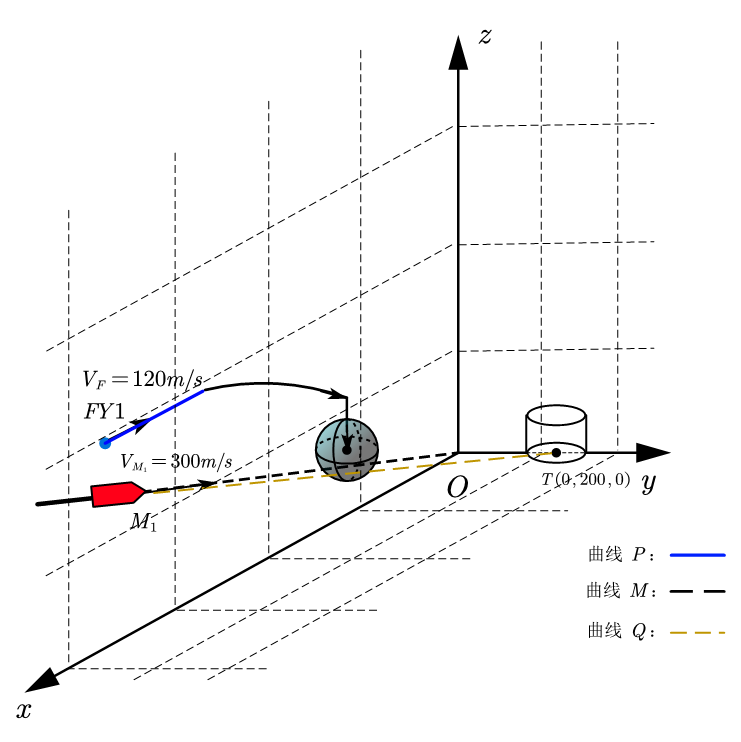
\includegraphics[width=0.5\textwidth]{烟幕干扰弹与导弹位置示意图.png}
    \caption{无人机投放烟幕干扰弹示意图 }
    \label{}
\end{figure}
参考FY1-M1-烟幕云团的位置示意图可建立以下模型：

\textbf{1.无人机，烟幕干扰弹和烟幕云团的运动模型}

无人机FY1向x轴反方向水平直线以速度$v_F=120m/s$的速度匀速飞行，其起始坐标为$F_0(17800,0,1800)$，$t_d=1.5s$后飞至$S(17620,0,1800)$投掷烟幕干扰弹,烟幕干扰弹先做水平初速度为$v_F$，竖直加速度为$g$（取9.8$m/s^2$）的抛物线运动，经过$\tau =3.6s$后，即$t_e=5.1s$时到达起爆点E起爆。烟幕干扰弹做抛物线运动时x坐标和z坐标的变化为：
\begin{equation}
    \Delta x=v_F\tau \quad    \Delta z=\frac{1}{2}g\tau ^2
\end{equation}

由此可计算出烟幕干扰弹起爆时的位置
\begin{equation}
    E=(17800-v_Ft_d-\Delta x,0,1800-\Delta z)
\end{equation}

干扰弹起爆后以速度$v_d$匀速下沉，可表示出云团中心的随时间$t$变化的坐标：
\begin{equation}
    C(t)=(E_x,E_y,E_z-3(t-t_e))
\end{equation}
其中 $E_x, E_y, E_z$ 分别为起爆点 $E$ 的 $x$、$y$、$z$ 坐标。

\textbf{2.导弹运动模型}

导弹$M_1$自$M_0$点以恒定速度$v_M$沿指向原点的方向飞行。其方向单位向量为：
\begin{equation}
    \overrightarrow{\eta}=-\frac{\overrightarrow{OM_0}}{|OM_0|}
\end{equation}

任意时刻导弹的位置$M_1(t)$满足：
\begin{equation}
    \overrightarrow{OM_1}=\overrightarrow{OM_0}+v_Mt\overrightarrow{\mu }
\end{equation}

结合上述两个公式可解出
\begin{equation}
 M_1(t)=(20000+300t\mu _x,0,2000+300t\mu _z)   
\end{equation}


\textbf{3.云团遮蔽判定}

判断球状烟幕云团是否能遮蔽真目标的关键在于判断导弹M1(设位置为$M_1$)与真目标T的连线线段TM$_1$是否能经过烟幕云团的球体B。
定义向量$\overrightarrow{TM_1}$，$\overrightarrow{TC}$，线段长度$L(t)=\| \overrightarrow{TM_1} \|  $，投影参数
\begin{equation}
    \lambda(t) =\frac{\overrightarrow{TM_1}\cdot \overrightarrow{TC}}{L^2(t)}
\end{equation}

定义C到线段TM$_1$的最小距离$d_{min}$，

(1)若$\lambda(t) \in [0,1] $，云团中心C点投影落在线段内，距离由叉乘公式计算：
\begin{equation}
    d_{min}(t)=\frac{\|\overrightarrow{TM_1}\times\overrightarrow{TC}  \| }{L(t) }
\end{equation}

(2)若C点投影在线段外，$\lambda >1$时，
\begin{equation}
    d_{min}=\|CM_1\| 
\end{equation}

(3)$\lambda <0$时，
\begin{equation}
    d_{min}=\|CT_1\| 
\end{equation}

三种情况的示意图\ref{fig:2}如下：
\begin{figure}[htbp]
    \centering
  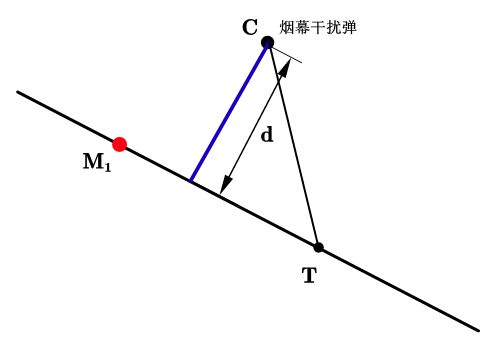
\includegraphics[width=0.3\textwidth]{情况一：0小于等于Lambda小于等于1.png}
  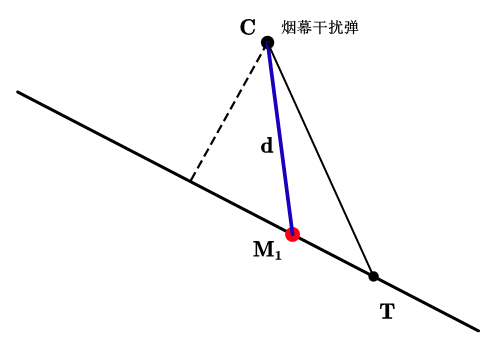
\includegraphics[width=0.3\textwidth]{情况二：Lambda大于1.png}
  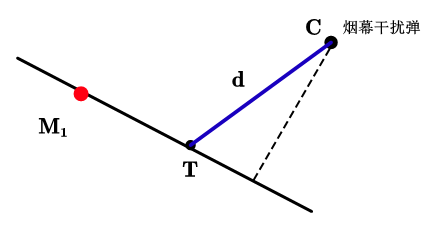
\includegraphics[width=0.3\textwidth]{情况三：Lambda小于0.png}
    \caption{云团中心-导弹-目标点位置情况分析}
    \label{fig:2}
\end{figure}


\textbf{4.遮蔽时长计算}

导弹在时刻 $t$ 被有效遮蔽的集合为：
\begin{equation}   
A=\{t \in [t_e, t_e + 20]\,\vert \, d_{min}(t) \leq R\}
\end{equation}
其中，R为烟幕云团的半径。

定义示性函数：
\begin{equation}
    \chi (t)=\mathbf{1}_A
\end{equation}

则遮蔽总时长即为:
\begin{equation}
    T_{total}=\int_{0}^{+\infty} \chi (t)  \,dt 
\end{equation}


\subsubsection{模型的求解}
根据前文所述的计算方法，可以判断出$d_{min}$是连续函数，我们先通过将时间离散为
$t_{i} = t_{e} + i\Delta t$（取 $\Delta t = 0.001\text{s}$，再结合二分法来计算出函数$f(t)=d_{min}(t)-R$的零点，最终得到K个能够遮蔽真目标的时间区间$\{[t_{L,k}, t_{R,k}]\}_{k=1}^{K}$，
总有效遮蔽时长为：
\begin{equation}
T_{\text{total}} = \sum_{k=1}^{K} (t_{R,k} - t_{L,k})
\end{equation}

具体计算步骤如下：

先计算出全部$f(t_i)$的值，将$f(t_i)\cdot f(t_{i+1})\leq 0$的粗略端点找出,$[t_i,t_{i+1}]$即为遮蔽区间的精确端点的邻域。为继续求得精确端点，采用二分法在粗略端点邻域迭代。将$f(t)$在逐个区间$[t_i,t_{i+1}]$上迭代N次（取N=80），容差$\epsilon =10^{-10}$,每次取中点$m=(t_i+t_{i+1})/2$并更新区间，直至满足邻域长度小于$\epsilon $或$f(m)=0$。

经计算，导弹进入烟幕云团的时间为9.39s(精确值为9.389247540)，导弹飞出云团的时间为9.45s(精确值为9.448088159)。而成功遮蔽的区间为[8.04,9.45](精确区间为[8.037890759,9.448088159])s，有效遮蔽时长$T_{total}=1.41s$。
\subsubsection{模型的分析与改进}
真目标实际为圆柱形区域，我们在计算中将真目标看做了一个点，我们现在扩展至整体圆柱。设真目标上任意一点为 $T = (x_T, y_T, z_T)$，
通过建构起真目标圆柱体的点阵，在圆柱体内不断更换采样点$T_k$进行 计算，得出每个采样点 $T_k$ 的有效遮蔽时间区间为 $[t_{k1}, t_{k2}]$（即 $t \in [t_e, t_e + 20]$ 且 $d(t) \leq R$ 的时间集合）。

由于整体圆柱被遮蔽的前提是所有采样点均被遮蔽，故圆柱的有效遮蔽时间区间为所有采样点遮蔽区间的交集：
\begin{equation}
    \Delta T = \bigcap_{k=1}^{N} [t_{k1}, t_{k2}]
\end{equation}
其中 $N$为总采样点数。

圆柱的有效遮蔽时长 $T_{\text{cov}}$ 为交集区间的长度之和，即若 $\Delta T = \bigcup_{i=1}^{n} [a_i, b_i]$（$[a_i, b_i]$ 为互不重叠的子区间），则：
\begin{equation}
    T_{\text{cov}} = \sum_{i=1}^{n} (b_i - a_i)
\end{equation}

求出遮蔽时间区间的交集，可以得出更为精细的时间区间和更准确的结果。
\begin{figure}[htbp]
    \centering
    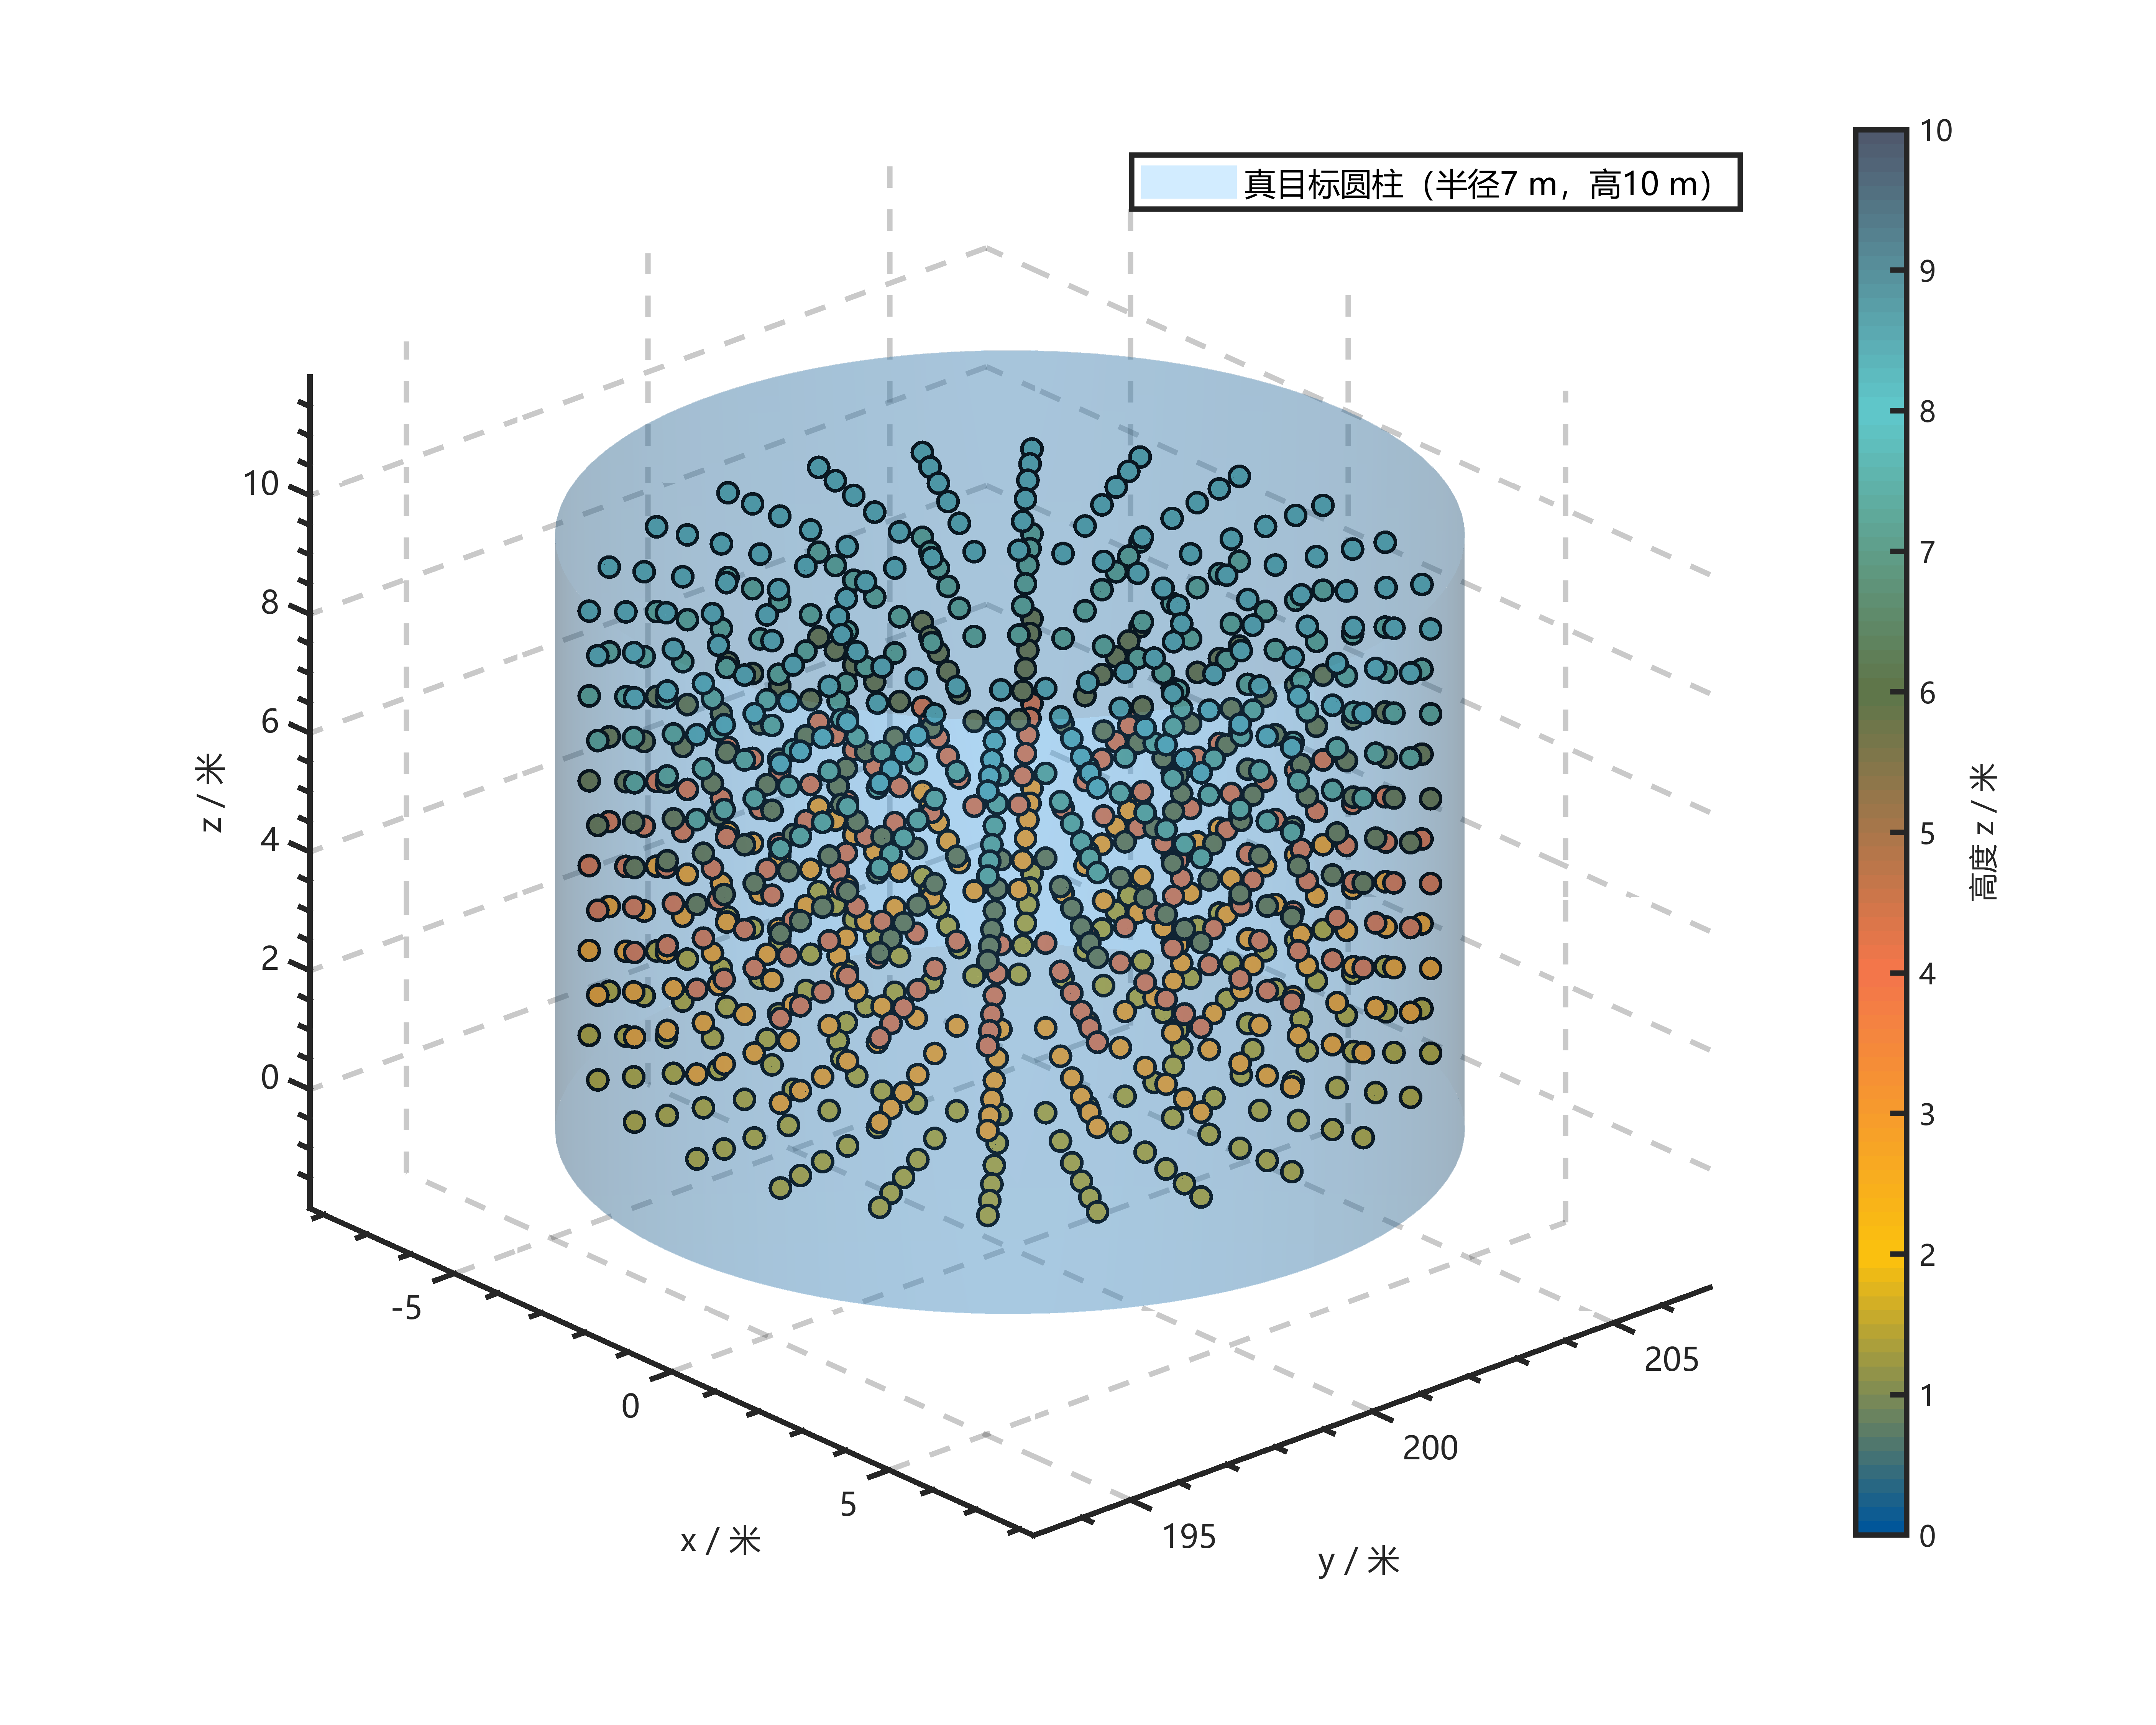
\includegraphics[width=0.6\textwidth]{圆柱体内取点情况.png}
    \caption{真目标圆柱体内取点图}
    \label{问题一取点展示}
\end{figure}

如图\ref{问题一取点展示}所示，我们总计取采样点14400个，展示其中10个采样点的有效遮蔽时间区间见下页表\ref{不同采样点的有效遮蔽时间}和图\ref{问题一模型优化特殊点结果展示}所示。
\begin{table}[htbp]
    \centering
    \caption{不同采样点的有效遮蔽时间}
    \label{不同采样点的有效遮蔽时间}
    \begin{tabular}{ccc}
        \toprule
        采样点坐标 &           有效遮蔽时间区间(s)        &   有效遮蔽时长(s)        \\
        \midrule
        (0,200,0)    &     [8.037890759 , 9.448088159]   &    1.410197399                      \\
        (0,200,10)    &     [7.987447071 , 9.448088159]   &   1.460641088                                 \\
        (0,193,10)    &     [7.967145320 , 9.448088159]    &   1.480942839                    \\
        (0,207,10)    &     [8.007527510 , 9.448088159]     &   1.440560649                    \\
        (7,200,5)    &       [8.016738460 , 9.448088159]     &  1.431349698                      \\
        (7,200,0)    &        [8.041529564 , 9.448088159]     &  1.406558595                    \\
        (7,200,10)    &       [7.991275177 , 9.448088159]      &  1.456812982              \\
        (0,193,5)    &       [7.993698968 , 9.448088159]   &      1.454389191              \\
        (0,193,0)    &      [8.019523903 , 9.448088159]     &     1.428564256             \\
        (0,200,5)   &      [8.013006057 , 9.448088159]       &     1.435082102              \\
        \bottomrule         
    \end{tabular}
    \end{table}

\begin{figure}[htbp]
    \centering
  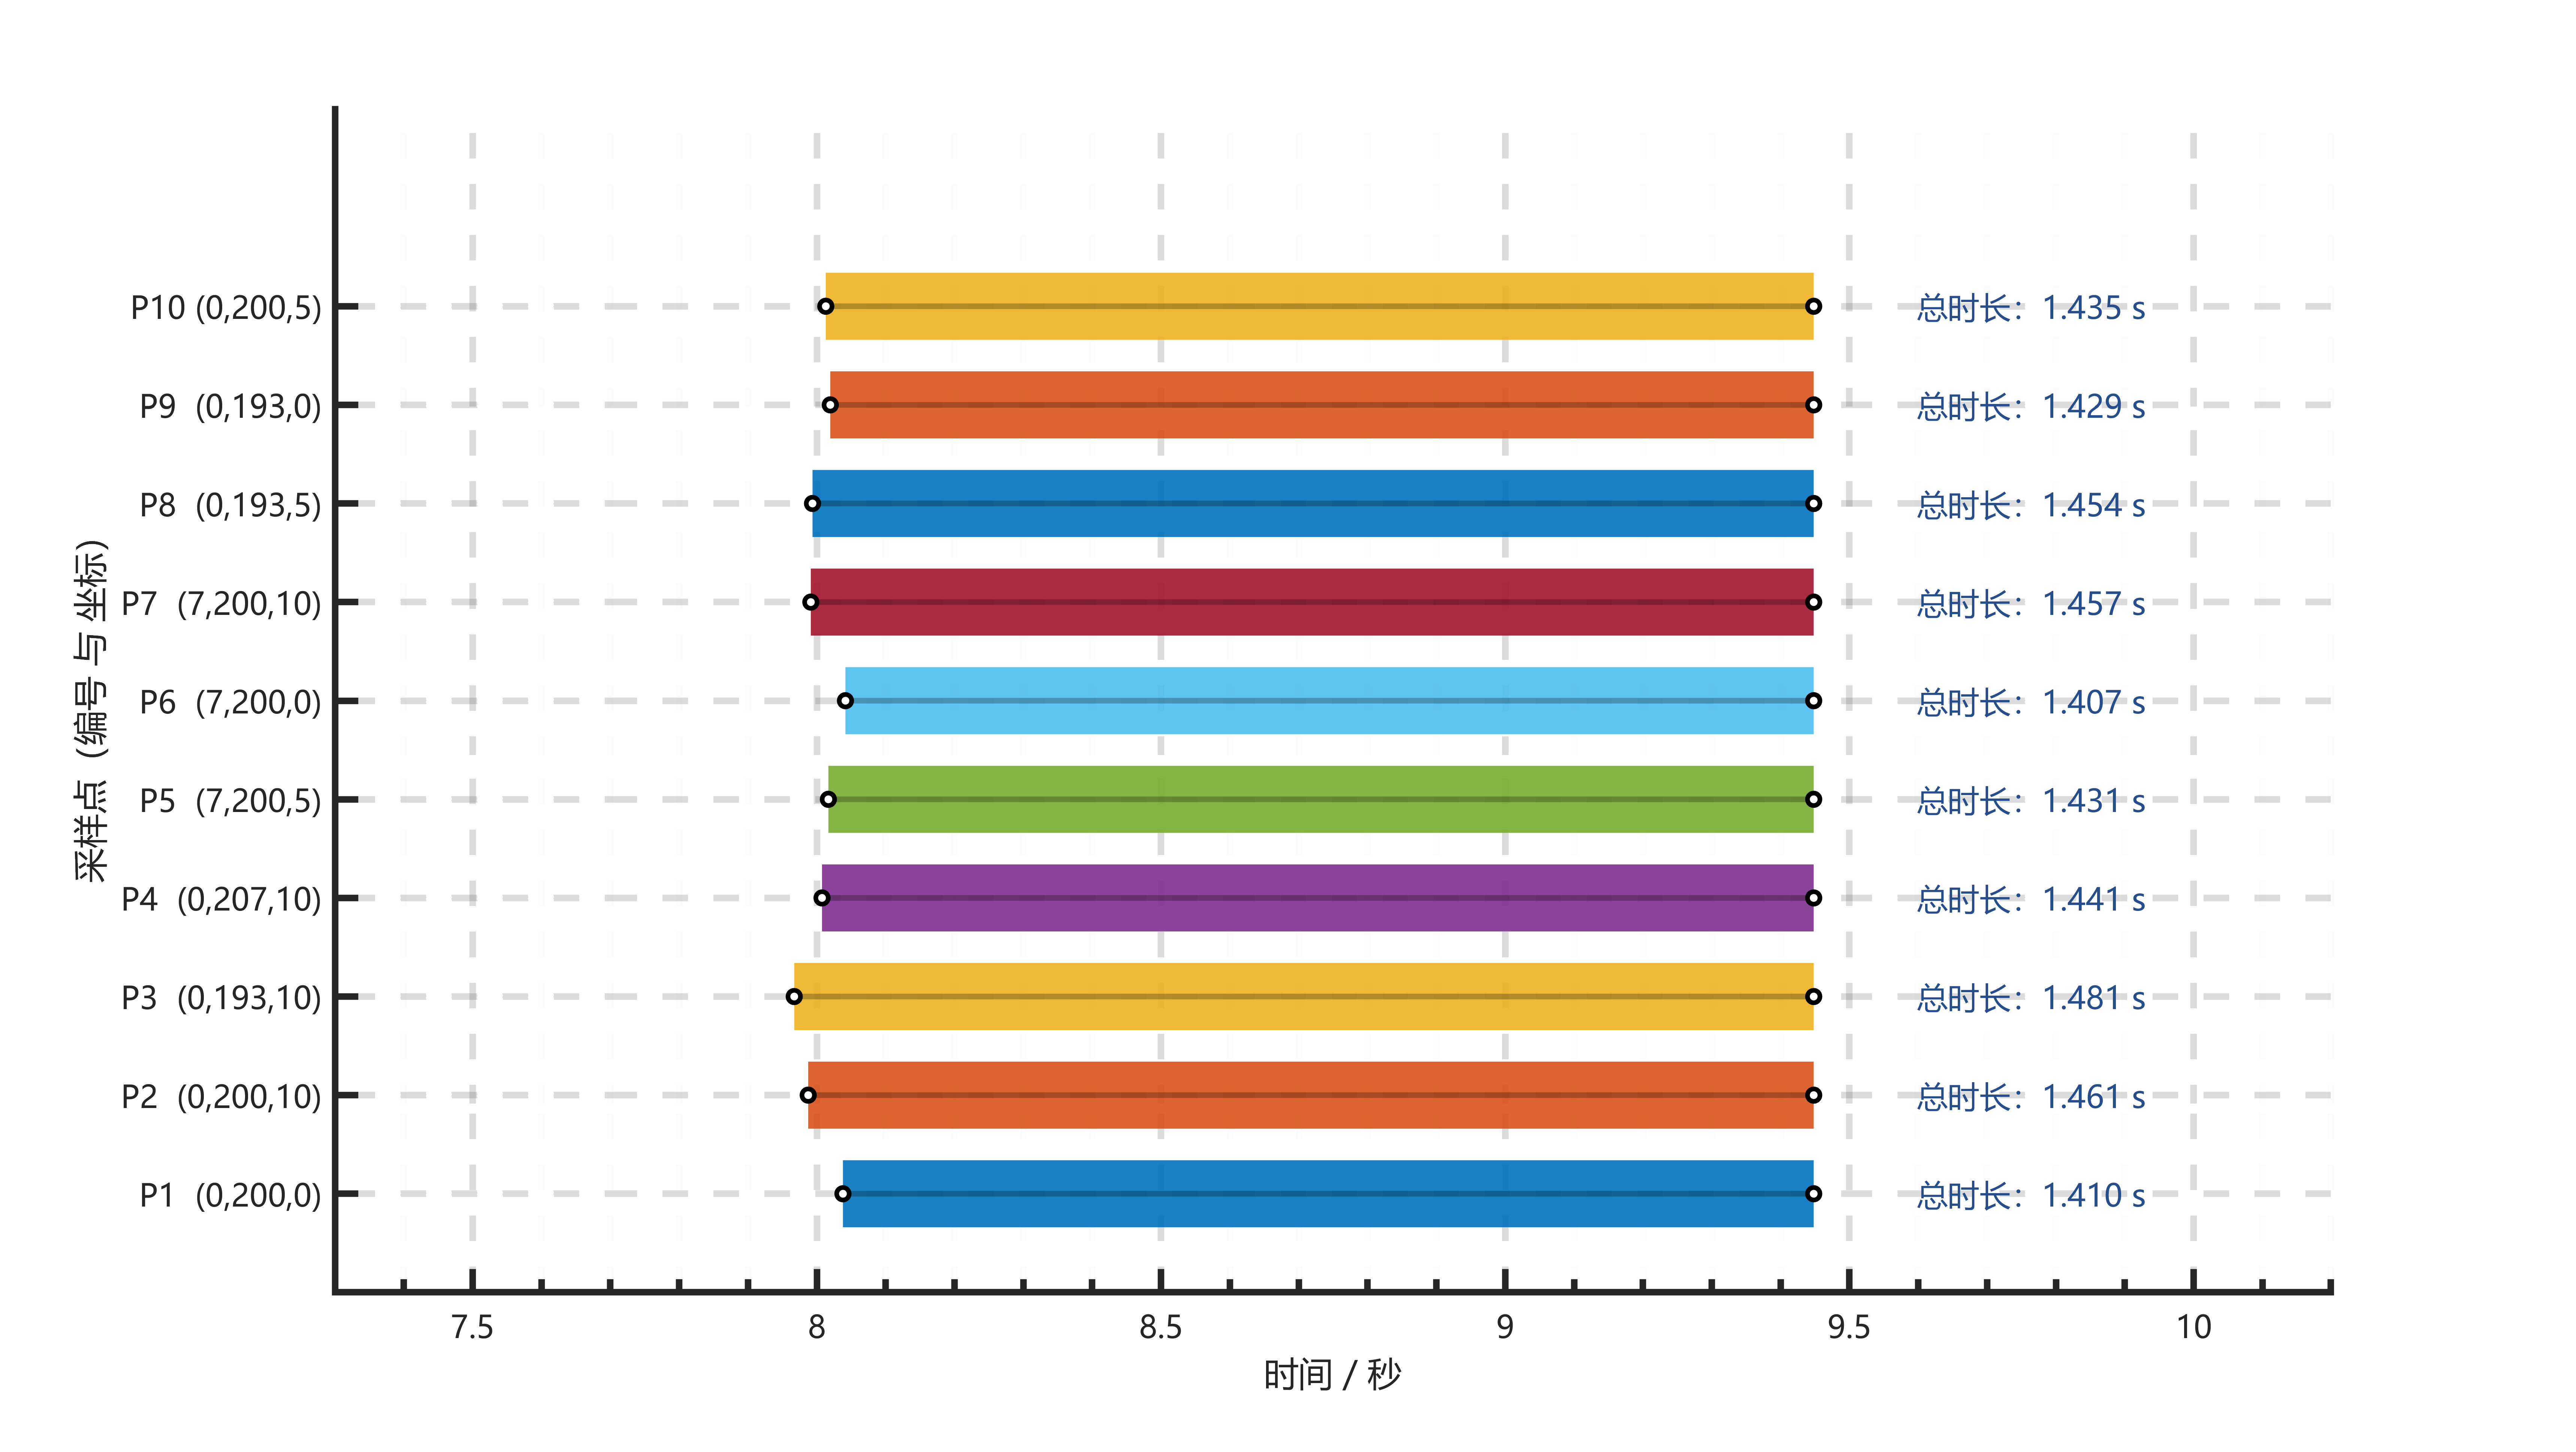
\includegraphics[width=0.9\textwidth]{十个点的遮蔽区间可视化.png}
    \caption{不同采样点的有效遮蔽时间可视化}
    \label{问题一模型优化特殊点结果展示}
\end{figure}

从选取的10组数据中可以发现以下规律：这10个采样点的有效遮蔽时间区间起始值相差不大，结束值完全相同，为9.448088159s。而计算发现导弹离开云团的时间为9.448088159s，显然，这是因为导弹离开云团后，烟幕弹将失去全部遮蔽作用。验证了结果的合理性。

求出14400个点的时间区间后取交集计算出$\Delta T$为[8.05 , 9.45]s,有效遮蔽时长$T_{cov}=1.39s$，验证发现，有效遮蔽时间区间长度小于表中选取的所有样本点，完全符合预期。
\subsection{问题二模型的建立与求解}
\subsubsection{模型的建立}
\textbf{1. 决策变量定义}

为得到无人机 FY1 投放单枚烟幕干扰弹对导弹 M1 的最长遮蔽时间，首先明确模型的决策变量，各变量物理意义及约束如下：
\begin{itemize}
    \item 无人机飞行速度为 $v$，需满足$[70,140]$。
    \item 无人机水平航向角为 $\phi$，即$x$ 轴正方向与无人机飞行方向的夹角，取值范围为$[0,2\pi]$。
    \item 无人机受领任务后至投放干扰弹的时间间隔为 $t_d$，即投放延迟时间，满足$t_d \geq 0$。
    \item 干扰弹从投放至起爆的时间间隔为 $\tau$，即起爆延迟时间，满足$\tau \geq 0$。
    \item 起爆时刻为 $t_e = t_d + \tau$，即受领任务后至干扰弹起爆的总时间。
\end{itemize}

\textbf{2. 无人机和干扰弹的运动轨迹}

无人机 FY1 初始位置$F_0(17800, 0, 1800)$，受领任务后以速度 $v_F$、航向角 $\phi$ 做等高度匀速直线飞行$z$ ,水平方向的单位航向向量可由 $\phi$ 确定：
\begin{equation}
    \mathbf{d} = (\cos\phi, \sin\phi, 0)
\end{equation}


在投放延迟时间 $t_d$ 后，无人机到达投放点 $S$，其坐标可表示为：
\begin{equation}
 S = F_0 + v_F t_d \mathbf{d} = \left( 17800 + v_F t_d \cos\phi,\  v_F t_d \sin\phi,\  1800 \right)   
\end{equation}

干扰弹脱离无人机后，做水平速度为$v_F$，竖直方向加速度为$g = 9.8 \, \text{m/s}^2$的抛物线运动。
在起爆延迟时间 $\tau$ 内，干扰弹水平位移为 $v_F \cdot \tau \cdot \mathbf{d}$，竖直位移由自由落体运动公式得 $-\frac{1}{2} g \tau^2$。则起爆点 $E$ 的坐标公式为：
\begin{equation}
    E = S + v  \tau  \mathbf{d} + \frac{1}{2} (0, 0, -g) \tau^2 
\end{equation}


代入 $S$ 的表达式展开后，烟幕干扰弹起爆点具体坐标为：
\begin{equation}
    E\left( 17800 + v_F (t_d + \tau) \cos\phi,\  v_F (t_d + \tau) \sin\phi,\  1800 - \frac{1}{2} g \tau^2 \right)
\end{equation}

同时需保证起爆点不低于地面（$z$ 坐标非负），即：
\begin{equation}
    1800 - \frac{1}{2} g \tau^2 \geq 0
\end{equation}

\textbf{3.烟幕云团与导弹运动轨迹}

烟幕干扰弹在E点起爆后，形成以 $E$ 为中心的球状云团，云团以 $v_c = 3 \, \text{m/s}$ 匀速下沉，且有效时间为20s，即$t \in [t_e, t_e + 20]$。云团中心 $C(t)$ 轨迹坐标为：
\begin{equation}
    C(t) = \left( E_x, E_y, E_z - v_c (t - t_e) \right)
\end{equation}
其中 $E_x, E_y, E_z$ 分别为起爆点 $E$ 的 $x$、$y$、$z$ 坐标。

由第一问的推导计算知，任意时刻 $t$ 的导弹位置 $M(t)$ 坐标为：
\begin{equation}
 M_1(t)=(20000+300t\mu _x,\, 0\, ,2000+300t\mu _z)   
\end{equation}

\textbf{4. 遮蔽判断准则}

真目标为圆柱形区域，我们可以先建立任意点目标的遮蔽判断逻辑，再扩展至整个圆柱体。设真目标上任意一点为 $T = (x_T, y_T, z_T)$，遮蔽的核心条件为：烟幕云团中心 $C(t)$ 到线段 $TM_1$ 上最近点的距离不超过云团半径 $R = 10 \, \text{m}$。

由第一问的模型推导可知，通过定义投影参数$\lambda(t) $，根据$\lambda $的值可以判断$d_{min}$的取值，进而判断出$d_{min}$在哪些时间区间下不大于$R$。

事实上，为判断整体圆柱是否被遮蔽，我们可以在圆柱体上均匀取点，按半径、周向、高度分别选取 $N_r$、$N_\theta$、$N_z$ 个采样点（半径向采样 $r_k = 7 \cdot \sqrt{\frac{k}{N_r + 1}}$，周向采样 $\theta_k = \frac{2\pi (k-1)}{N_\theta}$，高度向采样 $z_k = \frac{10 k}{N_z + 1}$，避免边界采样偏差），每个采样点 $T_k$ 的有效遮蔽时间区间为 $[t_{k1}, t_{k2}]$（即 $t \in [t_e, t_e + 20]$ 且 $d(t) \leq R$ 的时间集合）。

由第一问的模型推导知，圆柱的有效遮蔽时间区间为所有采样点遮蔽区间的交集：
\begin{equation}
    \Delta T = \bigcap_{k=1}^{N_{\text{total}}} [t_{k1}, t_{k2}]
\end{equation}
其中 $N_{\text{total}} = N_r \cdot N_\theta \cdot N_z$ 为总采样点数。

圆柱的有效遮蔽时长 $T_{\text{cov}}$ 为交集区间的长度之和，即若 $\Delta T = \bigcup_{i=1}^{n} [a_i, b_i]$（$[a_i, b_i]$ 为互不重叠的子区间），则：
\begin{equation}
    T_{\text{cov}} = \sum_{i=1}^{n} (b_i - a_i)
\end{equation}


\textbf{5. 目标函数}

问题二的核心目标是最大化圆柱目标的有效遮蔽时长，故目标函数为决策变量的函数：
\begin{equation}
    \label{问题二模型}
    \begin{aligned}
        &\max \quad T_{\text{cov}}(v, \phi, t_d, \tau) \\
        s.t.\quad &\begin{cases}
70 \leq v \leq 140 \\
0 \leq \phi \leq 2\pi \\
t_d \geq 0,\ 0\leq \tau \leq 20 \\
E_z = 1800 - \frac{1}{2} g \tau^2 \geq 0
\end{cases}
\end{aligned}
\end{equation}

\subsubsection{基于粒子群算法的模型求解策略分析}
粒子群算法(Particle Swarm Optimization,PSO)源于对鸟群、鱼群协同行为的建模，是一种全局启发式优化方法$^\text{\cite{ref10}}$。把可行解看作“粒子”，在有界连续解空间随机初始化一群粒子，每个粒子都记下自己历史上最好的位置和全群体里目前最好的位置。

算法迭代时，每个粒子都会依据三种规则来移动:一是保持原有运动趋势，二是向自己的历史最优靠拢，三是向群体最优靠拢，正如鸟群一样。由这三种因素共同决定粒子的“速度”和“位置”更新，并且要注意限制速度以避免速度变化过快，在每次更新变量的值后还要对越界变量回撤到边界或删除。最后每个粒子评估新位置的目标函数值，更新个体最优解以及群体最优解。
像这样进行多次循环，直到达到最大迭代次数或最优值长时间内不再改进即可输出最优解$^\text{\cite{ref2}}$。

粒子群算法在连续决策空间下无需依赖目标函数梯度且能灵活处理约束条件。而问题二是一个搜索空间连续，但缺乏显式数学表达，易陷局部最优的问题。PSO算法能够仅通过调整参数自动引导搜索方向，结合个体与全局最优平衡探索与利用以较好的避免陷入局部最优，故粒子群算法是求解该问题的极佳算法$^\text{\cite{ref2}}$。基于粒子群算法求解问题二模型的步骤如下：
\paragraph{Step 1 决策变量与可行域}
根据模型建立部分的讨论可知，决策向量取 \( \mathbf{x} = [v, \phi, t_d, \tau] \)：无人机水平航速 \( v \in [70, 140] \, \text{m/s} \)、航向角 \( \phi \in [0, 2\pi] \)、投放时间 \( t_d \in [0, 60] \, \text{s} \)、干扰弹从投放到爆开的间隔时间 \( \tau \in [0, 15] \, \text{s} \)；其余场景参数按题意：导弹速率 \( v_M=300 \, \text{m/s} \)、云团下沉速度 \(v_d= 3 \, \text{m/s} \)、云团半径 \( R=10 \, \text{m} \)、圆柱真目标中心 \( (0, 200) \)、半径 \( 7 \, \text{m} \)、高度 \(10 \, \text{m} \)。

\paragraph{Step 2 适应度函数}
适应度函数用于评估模型的优劣。对每个粒子给定的 \( \mathbf{x} \)，先由 FY1 位置与 \( (v, \phi, t_d, \tau) \) 表示出起爆点 \( E \)；随后在圆柱体内均匀采样若干点，分别计算每个点在 \( [t_e, t_e + 20] \) 内被烟幕云团遮蔽的时间区间，并对所有点的时间区间取交集得到整体圆柱被完全遮蔽的时间段，总长度为 \( T_{\text{cov}} \)。

\paragraph{Step 3 初始化粒子群}
由分析可确定搜索空间$\varOmega=[70,140]\times[0,2\pi]\times[0,60]\times[0,15]$。在上述搜索空间内均匀随机生成 \( N_p \) 个粒子位置 $\mathbf{x}\in \varOmega $，设置初始速度$\mathbf{v}=\mathbf{0}$，并计算初始适应度，设置每个粒子的个体最优 \( \mathbf{P} \) 与全局最优 \( \mathbf{G} \)。


\paragraph{Step 4 群体进化}
粒子群总迭代次数为$K$，记第k次迭代后第n个粒子为$\mathbf{x}_n^{(k)}$，惯性权重 \( \omega  \) 线性递减，设$\omega_{min}$，$\omega_{max}$。第k次迭代的$\omega_{k}$表达式为：
\begin{equation}
    \omega_k=\omega_{max}-\frac{\omega_{max}-\omega_{min}}{K}k
\end{equation}
粒子位置更新公式为：
\begin{equation}
    \mathbf{v}_n^{k+1} = w_k \mathbf{v}_n^k + c_1 \mathbf{r}_1 (\mathbf{P}_n^k - \mathbf{x}_n^k) + c_2 \mathbf{r}_2 (\mathbf{G}^k - \mathbf{x}_n^k)
\end{equation}
\begin{equation}
    \tilde{\mathbf{x}}_n^{k+1} = \mathbf{x}_n^k + \mathbf{v}_n^{k+1}, \quad \mathbf{x}_n^{k+1} = \Pi_\Omega(\tilde{\mathbf{x}}_n^{k+1})
\end{equation}
其中，$\mathbf{r}_1,\mathbf{r}_2$均为4维随机数常值向量，每个维度的取值均在0-1之间。$c_1,c_2$分别为个体、群体的学习因子。$\Pi_\Omega(\cdot)$是回归边值运算，即当粒子位置超出搜索空间时，将粒子的值重置为边界值，以确保每次迭代后的粒子位置都在搜索空间内。\(\tilde{\mathbf{x}}\)为过渡值。

随后重新计算每个粒子的适应度并更新本次迭代后的 \( \mathbf{P} , \mathbf{G} \)。

\paragraph{Step 5 结果输出}
迭代结束后取 \( \mathbf{G} = [v, \phi, t_d, \tau] \)，计算出 \( E \)、\( t_e \)。在圆柱体内按照前文讨论的采样规则均匀选取$N_{total}$个点，得到每个点的遮蔽时间区间$\Delta T$,进而得到$T_{cov}$。
\begin{figure}[htbp]
    \centering
    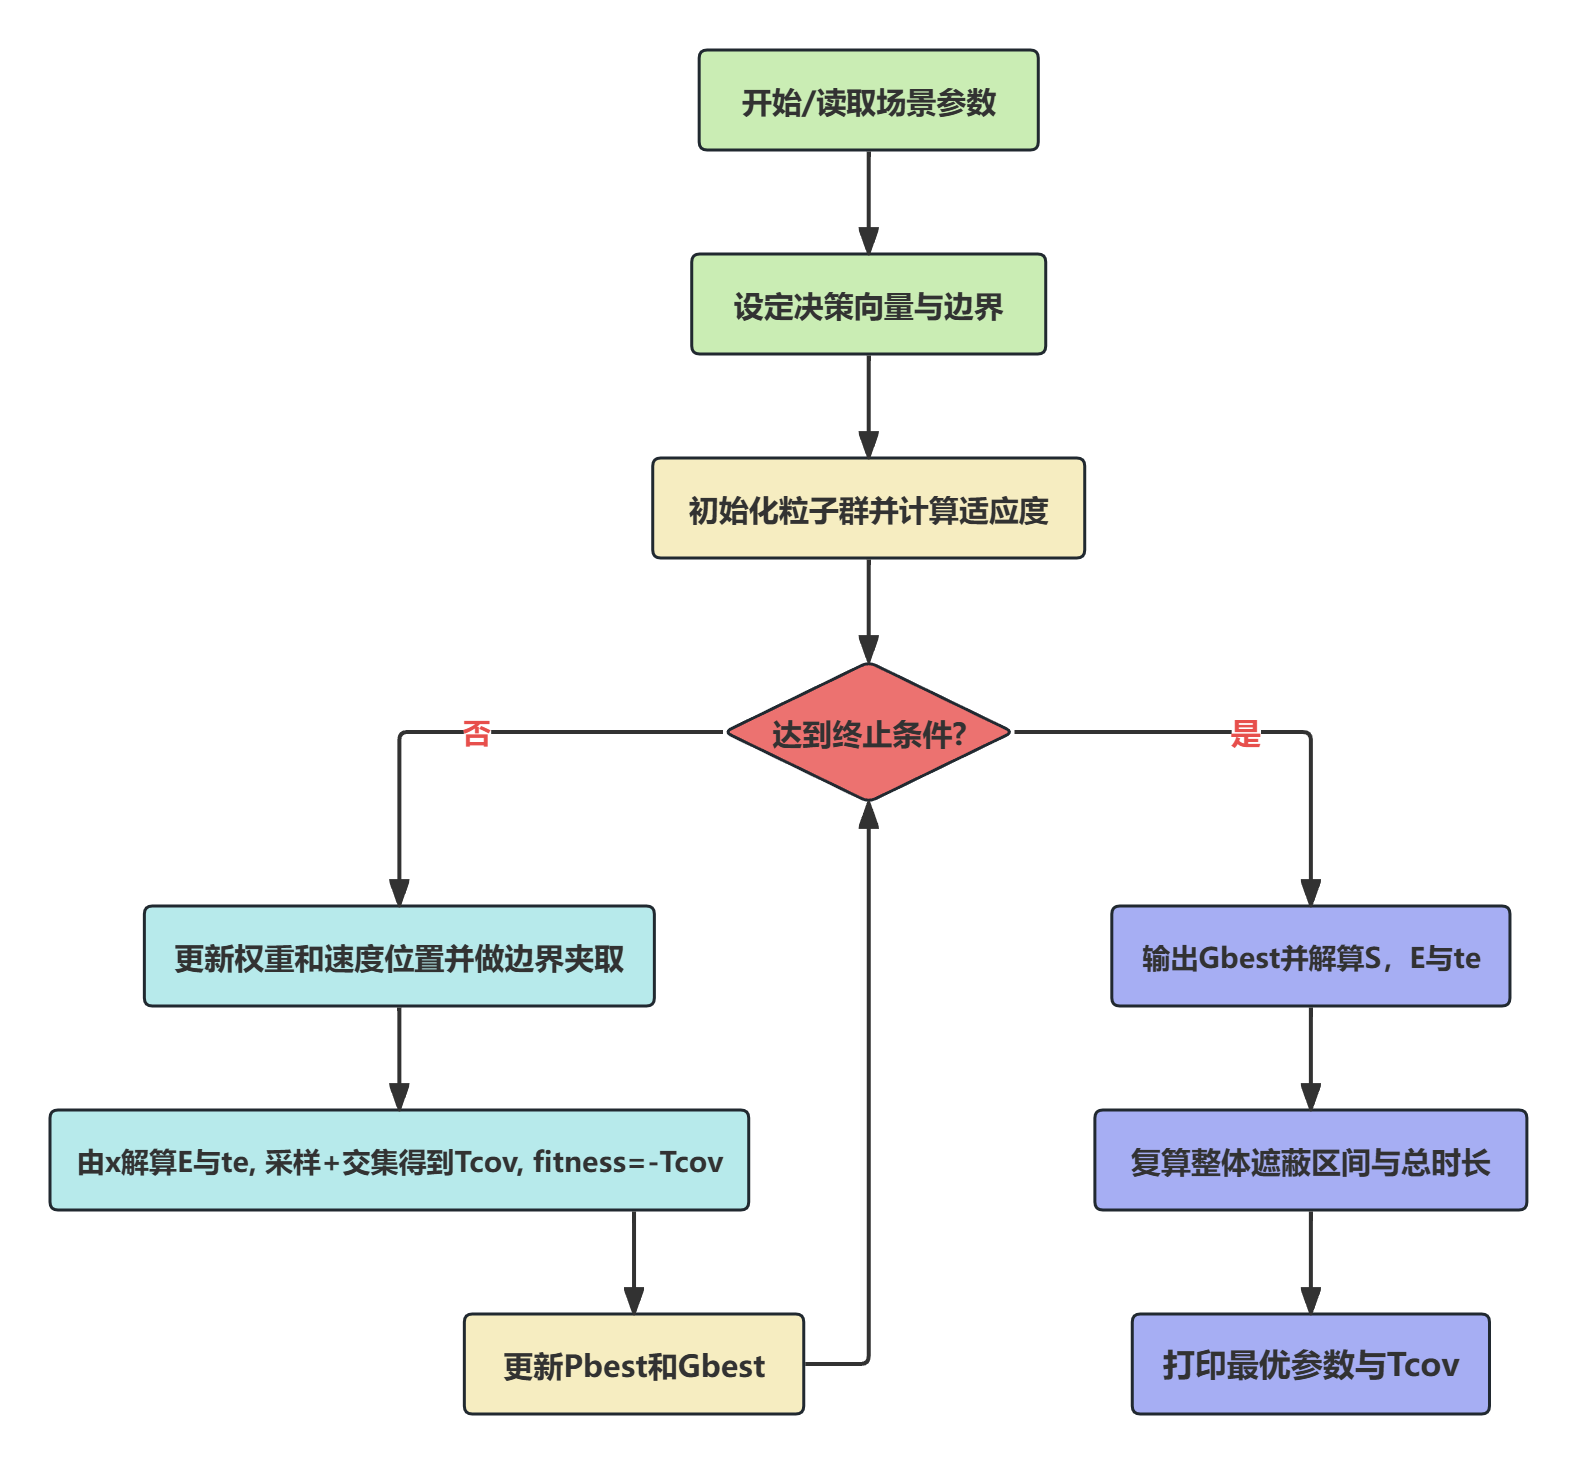
\includegraphics[width=0.5\textwidth]{PSO流程图.png}
    \caption{问题二求解流程图}
    \label{问题二求解流程图}
\end{figure}

\subsubsection{模型的求解与结果分析}
    根据前文所述的计算方法，我们通过粒子群优化算法来求解方程\ref{问题二模型},求得FY1 的飞行方向$\phi $、飞行速度$v$、烟幕干扰弹投放点$S$、烟幕干扰弹起爆点$E$。结果展示如下表所示：
    \begin{table}[htbp]
    \centering
    \caption{问题二核心结果}
    \label{问题二核心结果}
    \begin{tabular}{cccc}
        \toprule
        飞行方向$\phi $ (rad)& 飞行速度 $v$ (m/s)   & 烟幕干扰弹投放点$S$ &烟幕干扰弹起爆点 $E$\\
        \midrule
        0.120  & 139.8 &(17801.4, 0.2, 1800.0)   & (17902.5, 12.4, 1797.4) \\
        \bottomrule
    \end{tabular}
    \end{table}

    同时计算出烟幕干扰弹投放时间$t_d$ ，烟幕干扰弹起爆时间$t_e$ ，烟幕云团遮蔽时间$T_{cov}$结果展示如下表：
     \begin{table}[htbp]
    \centering
    \caption{问题二附加结果}
    \label{问题二附加结果}
    \begin{tabular}{ccc}
        \toprule
        烟幕干扰弹投放时间$t_d$ (s) &烟幕干扰弹起爆时间$t_e$ (s) &烟幕云团遮蔽时间$T_{cov}$(s)\\
        \midrule
        0.01  & 0.738 &4.64\\
        \bottomrule
    \end{tabular}
    \end{table}
\newpage
我们分析表\ref{问题二核心结果}和表\ref{问题二附加结果}发现以下规律：
\begin{itemize}
    \item 无人机飞行角度近似与沿x轴负方向运动，这是因为真目标底面的中心的坐标为(0,200,0)，相对导弹和无人机位置来说近似于在原点。无人机，导弹和真目标之间的连线在XOY平面的投影近似为同一条直线，故为了有效遮蔽，无人机的飞行角度一定较小。
    \item 无人机投放干扰弹的时间为0.01s，经0.738s后起爆，在1s之内就完成了投放和起爆两个动作。经演算发现，这是因为导弹M1与无人机FY1在x方向上的距离只有2200m，当FY1以139.8m/s的速度大小，0.120rad的速度方向飞行时，约5s后，即第5.7s时便会和M1大致相遇，云团在第1s内起爆而有效遮蔽时长为4.64s，在M1飞出云团范围后遮蔽作用失效。故该结果的合理性得到验证。
\end{itemize}

使用粒子群算法解决上述模型得到求解结果后，需要对结果进行合理性验证。图\ref{粒子群算法决策变量收敛曲线}展示了该算法四个决策变量的迭代收敛曲线。
\begin{figure}[htbp]
    \centering
  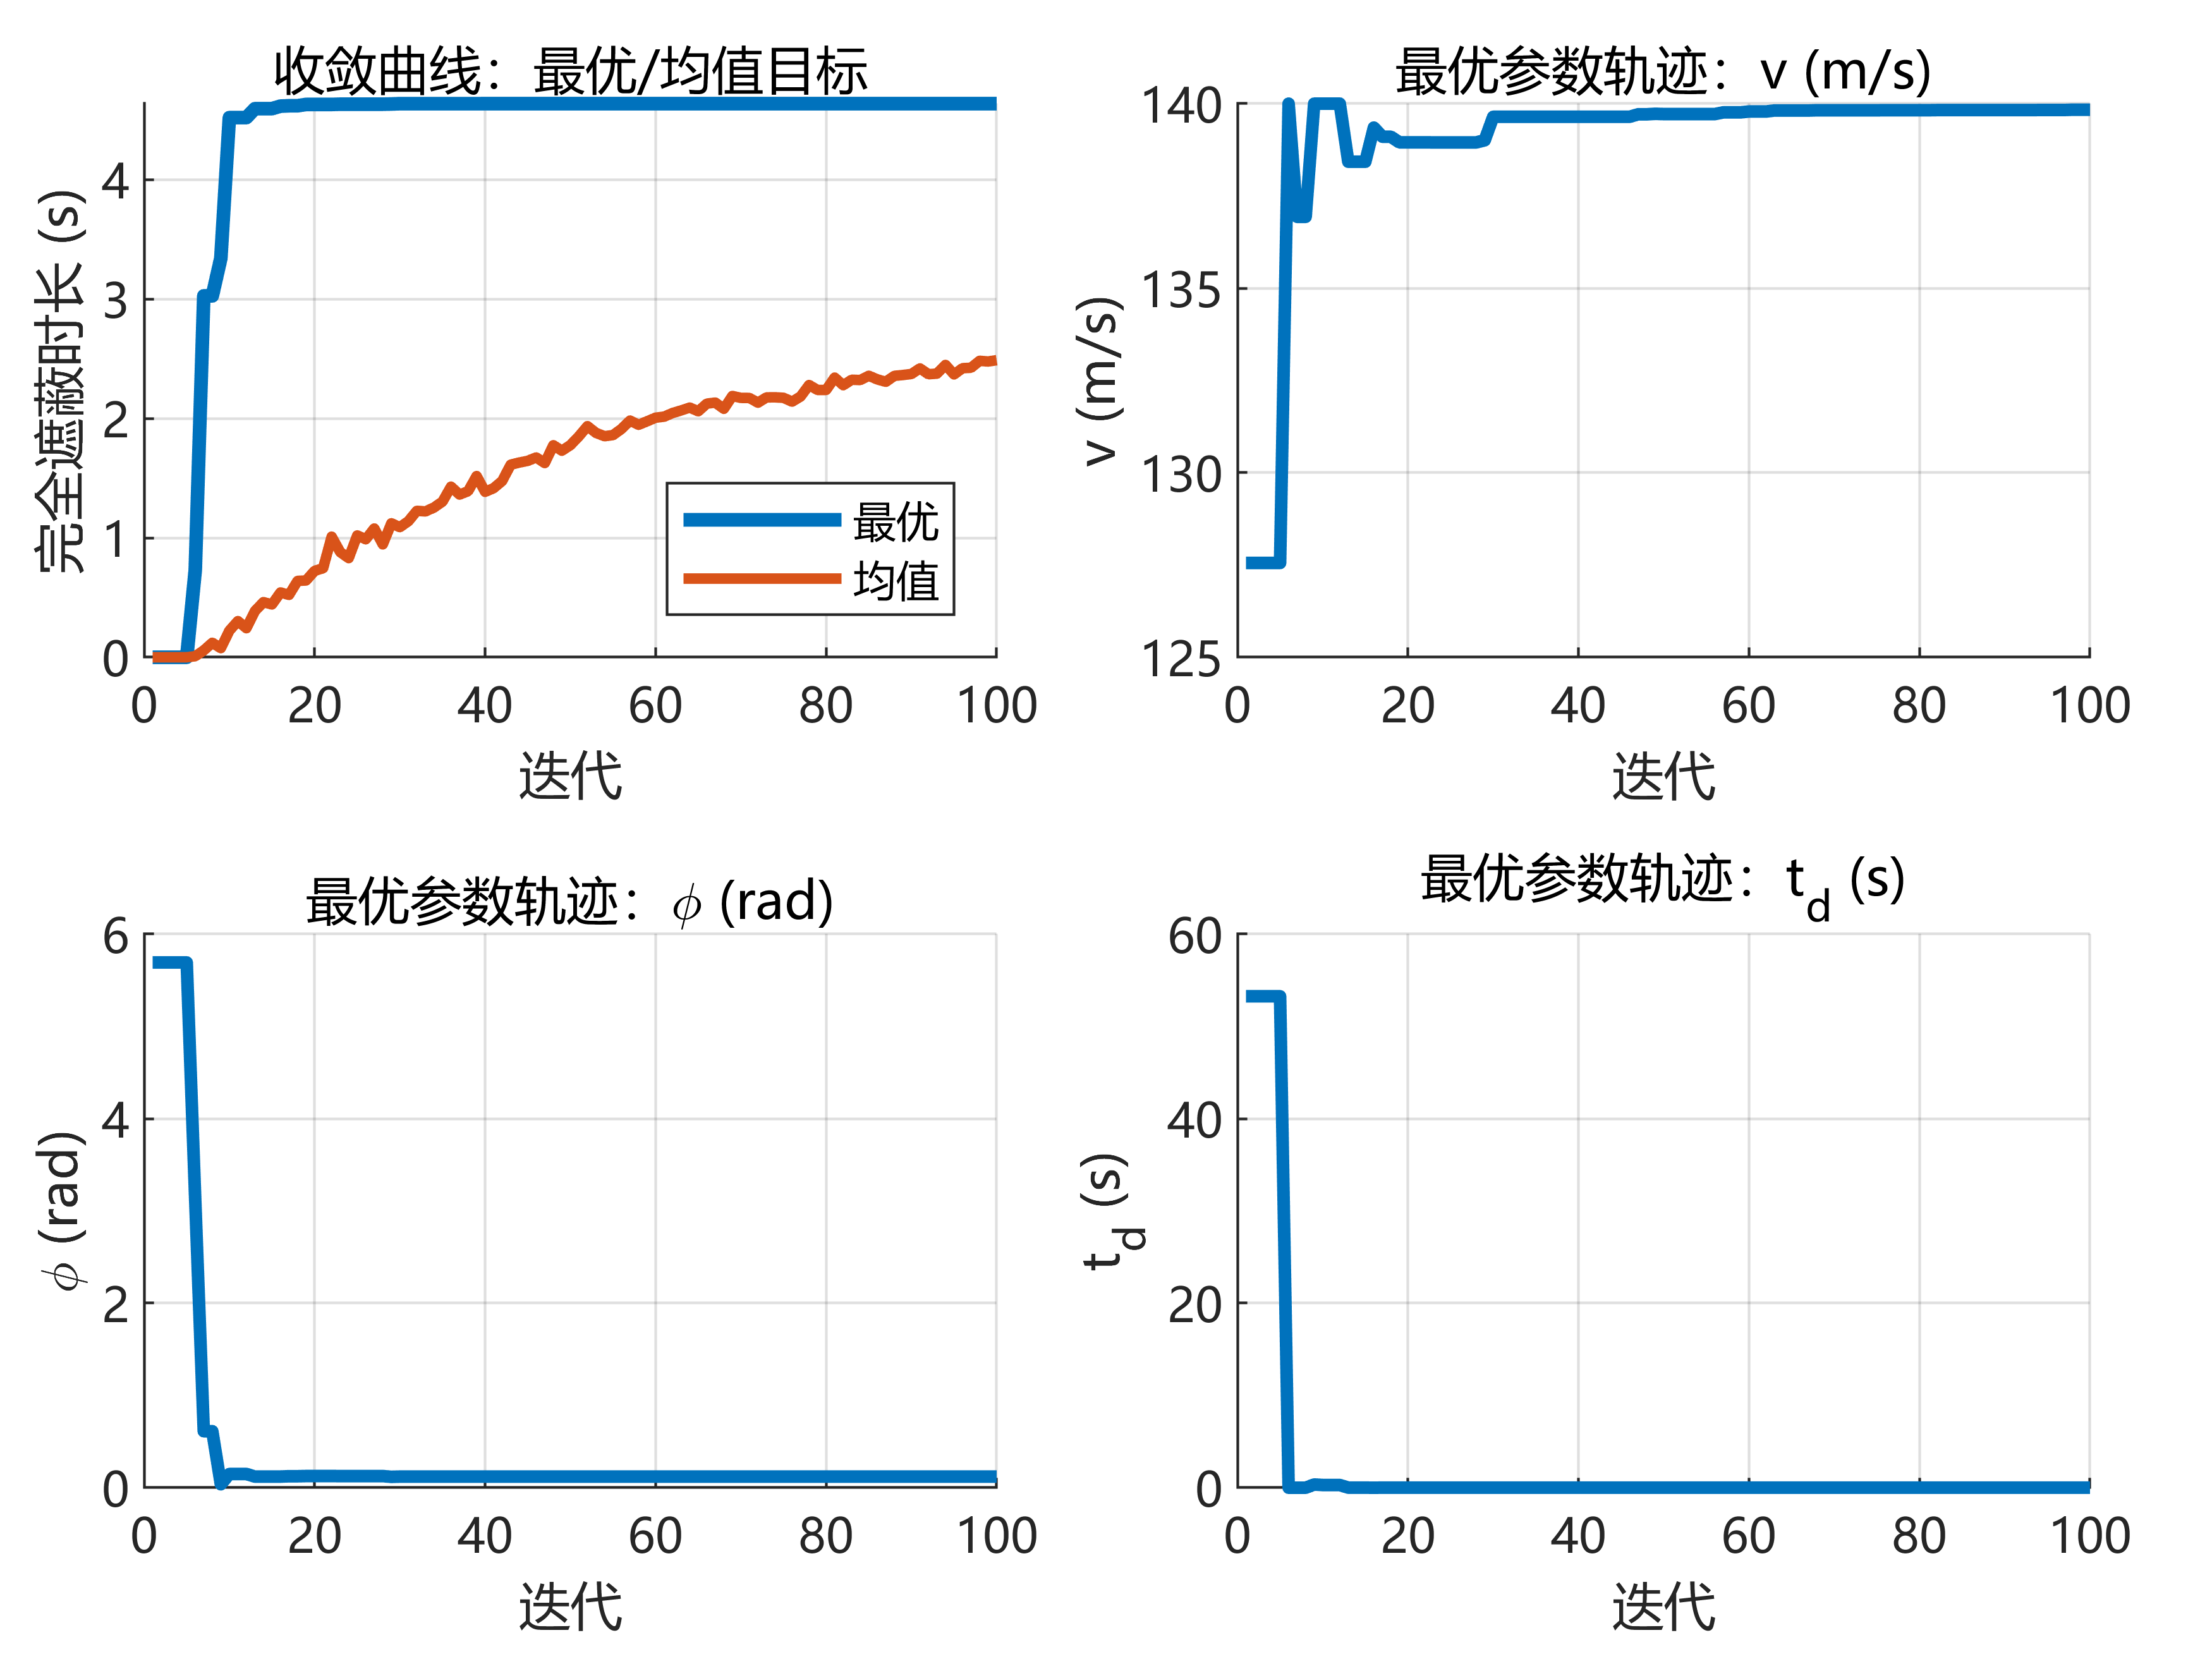
\includegraphics[width=0.6\textwidth]{PSO各参数收敛曲线.png}
    \caption{问题二决策变量收敛曲线}
    \label{粒子群算法决策变量收敛曲线}
\end{figure}

结合图6可以发现，粒子群算法在15次迭代左右就已经快速收敛到一个较优解，并且在15次后趋于平稳。经过多次实验，我们发现粒子群算法所展示的良好收敛性，再一次证明了我们选择粒子群算法的合理性。

\begin{figure}[htbp]
    \centering
    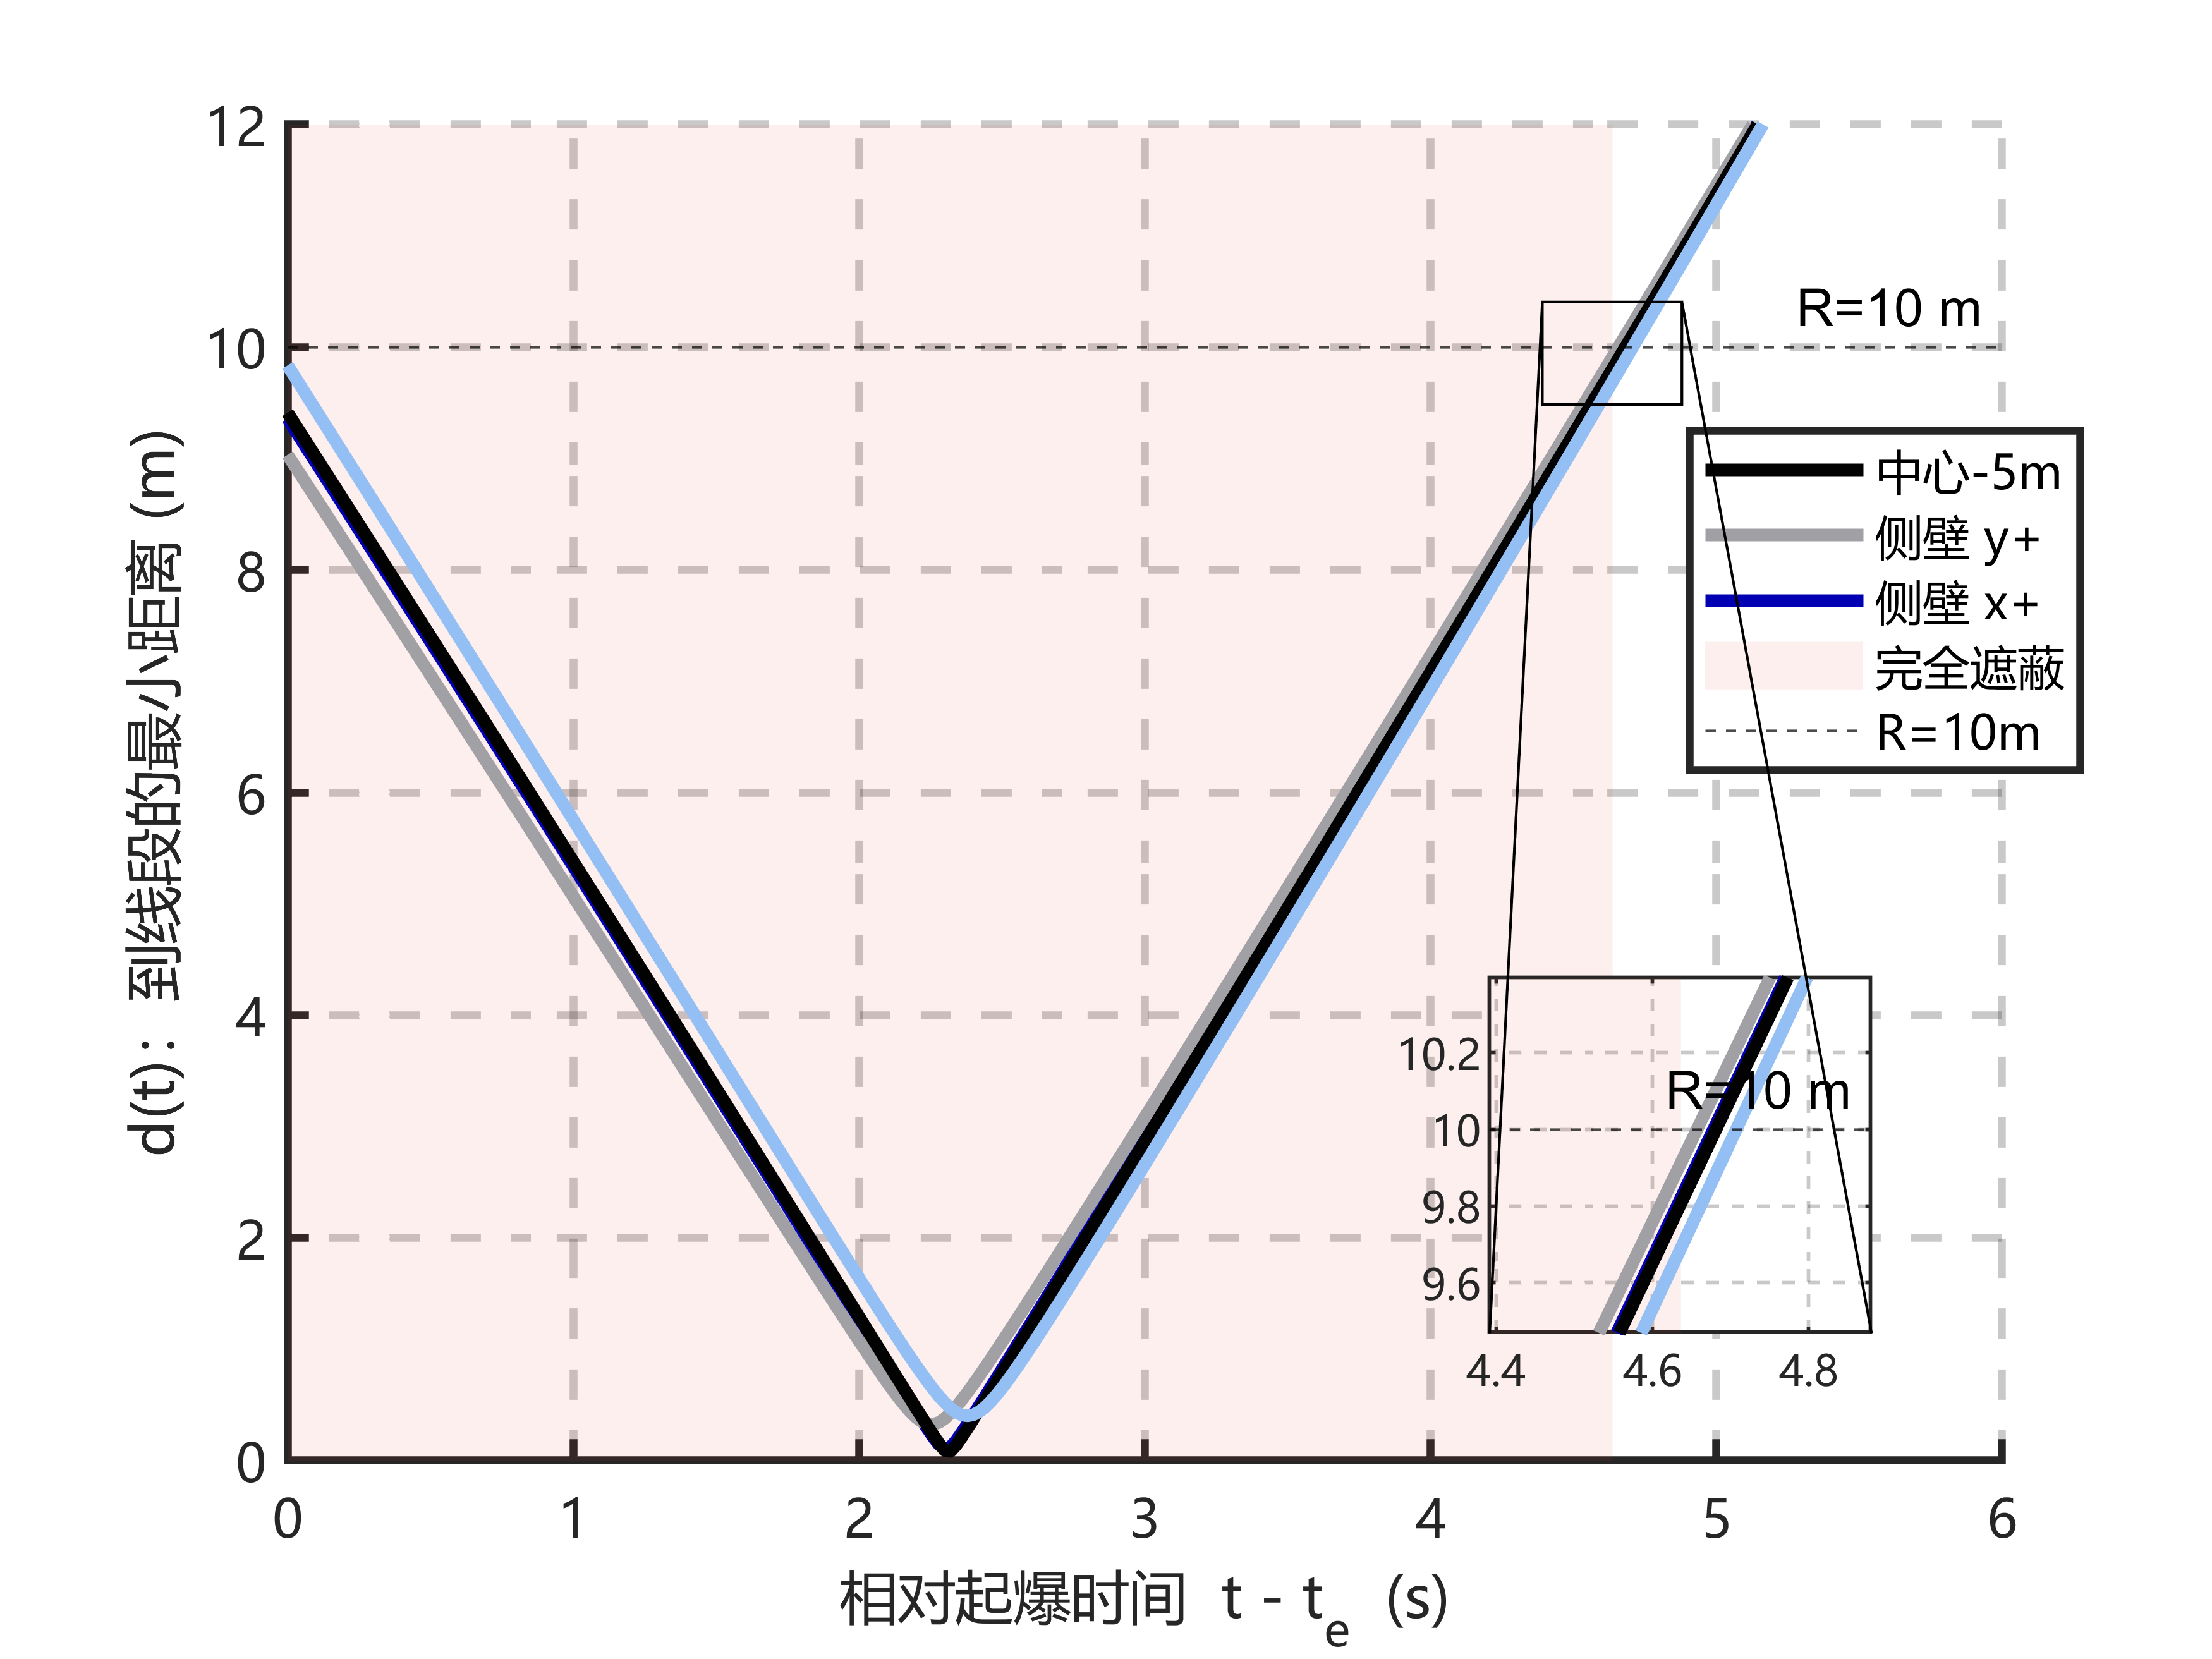
\includegraphics[width=0.6\textwidth]{代表点距云团—导弹连线的最小距离（0–6 s；阴影=完全遮蔽）.png}
    \caption{云团距三类采样点—导弹连线的最小距离}
    \label{云团距三类采样点—导弹连线的最小距离}
\end{figure}
\newpage
图\ref{云团距三类采样点—导弹连线的最小距离}是在对真目标圆柱体均匀取点后，计算不同位置上的点随干扰弹起爆后的时间，云团中心到导弹-采样点的线段的最小长度的变化。通过分析该图，我们可以得到以下结论：
\begin{itemize}
    \item 起爆时，云团中心到圆柱体侧壁x+上的某采样点—导弹的最小距离约为$R=10m$，说明该起爆时间设计合理。
    \item 4.64s时，由放大图可以看到，云团中心到圆柱体侧壁y+上的某采样点-导弹的最小距离约为$R=10m$，反映遮蔽时间的计算的正确性。
    \item 在起爆时和4.64s时刻上，柱体中心点所代表的曲线均夹在侧壁所代表的两条曲线之间。这启发我们，在接下来的问题中，在真目标上取采样点时，可能并不需要在圆柱体内部取点，只取边界点即可满足需要并极大的减少了循环次数和运算量。
\end{itemize}

\subsection{问题三模型的建立与求解}

\subsubsection{模型的建立}
\begin{figure}[htbp]
    \centering
    \label{}
    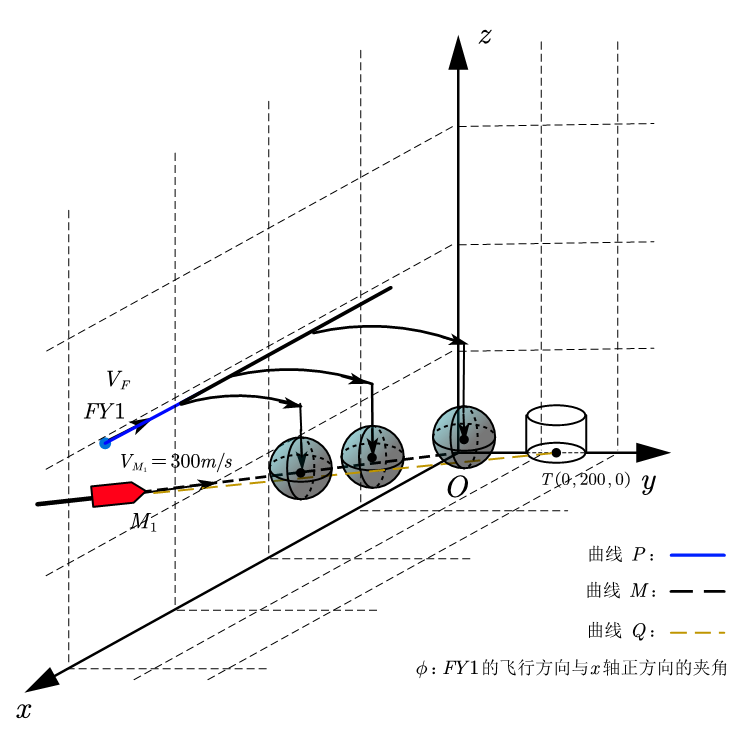
\includegraphics[width=0.5\textwidth]{FY1投放三枚烟幕干扰弹运动轨迹示意图.png}
    \caption{无人机投放烟幕干扰弹示意图 }
\end{figure}
参考下页的FY1-M1-三个烟幕云团的位置示意图8可建立以下模型：

\textbf{1.决策变量的定义}

相较于问题二，问题三中FY1无人机多投放了两枚烟幕干扰弹，决策变量数量相应增加，各变量的物理意义定义如下：
\begin{itemize}
    \item 无人机飞行速度\( v \)，其取值范围需满足\( v \in [70, 140] \)
    \item 无人机飞行角度$\phi $，满足$0\leq \phi \leq 2\pi$
    \item 第i枚烟幕干扰弹投放时间$t_i$（i=1,2,3）
    \item 第i枚烟幕干扰弹从投放到起爆的时间$\tau_i$，满足$0\leq \tau_i \leq 20$（i=1,2,3）
\end{itemize}

\textbf{2.模型复用与约束条件}

问题二中所建立的无人机-干扰弹运动轨迹模型、烟幕云团-导弹运动轨迹模型以及遮蔽判断准则在问题三中完全适用，仅需对部分参数进行补充替换：
\begin{itemize}
    \item 将问题二中的单枚干扰弹投放时间\( t_d \)替换为三枚干扰弹的投放时间\( t_i \)（\( i=1,2,3 \)，分别对应第1、2、3枚干扰弹）
    \item 将问题二中的单参数\( \tau \)替换为三枚干扰弹的对应参数$\tau_i$（\( i=1,2,3 \)，分别对应第1、2、3枚干扰弹）
\end{itemize} 

由问题二的模型推导可知，我们可以最终可以分别得出三枚干扰弹的遮蔽时间区间\(\Delta  T_i=\bigcap_{k=1}^{N_{\text{total}}} [t_{k1}, t_{k2}]\)（\( i=1,2,3 \)）。总遮蔽区间为三枚干扰弹遮蔽区间的并集，即：
\begin{equation}
    \Delta T= \bigcup _{i=1}^3\Delta T_i
\end{equation}

有效遮蔽时长 $T_{\text{cov}}$ 为遮蔽时间$\Delta T$的区间长度之和，即若 $\Delta T = \bigcup_{i=1}^{n} [a_i, b_i]$（$[a_i, b_i]$ 为互不重叠的子区间），则：
\begin{equation}
    T_{\text{cov}} = \sum_{i=1}^{n} (b_i - a_i)
\end{equation}

基于上述分析，可建立与问题二结构相似的非线性规划模型，但需额外增加每架无人机投放两枚烟幕干扰弹的时间间隔至少为1s的约束条件。最终建立的模型如下：
\begin{equation}
\begin{aligned}
& \max \quad T_{\text{cov}}(v, \phi, t_1,t_2,t_3, \tau_1,\tau_2,\tau_3)  \\
s.t.\quad &\begin{cases}
70 \leq v \leq 140 \\
0 \leq \phi \leq 2\pi \\
t_i \geq 0,\ 0\leq \tau \leq 20 \ (i=1,2,3) \\
E_z = 1800 - \frac{1}{2} g \tau_i^2 \geq 0\ (i=1,2,3)\\
t_2 \geq t_1+1 \\
t_3 \geq t_2+1
\end{cases}
\end{aligned}
\end{equation}


\subsubsection{粒子群-差分进化融合算法（PSO-DE）在模型求解中的运用}
优化算法在解决复杂问题时能够发挥重要作用，其中粒子群算法与差分进化算法作为两种经典的算法，广泛应用于全局优化问题。本节将粒子群算法与差分进化算法相结合，旨在充分发挥二者的优势，提高算法的收敛速度与精度，从而为该复杂优化问题的求解提供更有效的解决方案$^\text{\cite{ref3}}$。

差分进化算法（Differential Evolution, DE）是源于遗传算法、受生物进化启发的群体智能优化算法，适合在多维连续搜索空间中寻找全局最优解。​它以种群为基础进行优化：在初始种群的基础上通过变异、交叉、选择三步进行迭代改进。DE 的优势是参数少、实现简单、全局搜索能力强，但还不能完全避免陷入局部最优陷阱$^\text{\cite{ref2}}$。

PSO-DE是在PSO框架上引入差分进化中的变异和交叉方法，对PSO算法进行补充改进:先按常规的PSO计算得到新的群体最优，然后从群体中挑选一部分“精英粒子”(不必全部都是较优粒子)，对这些粒子再使用DE进行扰动与重组。具体做法是:用当前解朝向群体最优再叠加两个随机个体差分的方向作为变异，然后按一定的交叉概率生成候选解，用更好的解来替换原解，由于本问题是8维模型，依据Gamperle等人的数值实验，NP的取值应在[24,64]，F取0.6，CR的取值范围是[0.3,0.9]为较好的选择$^\text{\cite{ref11}}$。

这种融合算法的优点是保留PSO前期全局搜索、实现快速收敛的优点，同时利用DE的定向扰动与自适应步长来增强跨盆地跳跃和精确找到最优解的能力，从而降低陷入局部最优解的风险，提升复杂问题上的处理能力。代价是每一代的计算量略增，且需要额外调节少量DE参数(如差分放大系数与交叉率)。

对于该模型的求解，我们一开始使用粒子群算法求解出每个采样点最长遮蔽时间。但是我们在不断调整学习因子、种群数量、迭代次数等参数的过程中发现，该算法迭代速度较慢，求解得到的遮蔽时间约为4.77s，与问题二投放单枚烟幕干扰弹的结果相差不大，说明该算法极有可能陷入了局部最优解。为改善求解效果，我们采取了以下两项优化措施：
\begin{enumerate}
    \item 采样方式优化：利用凸集上凸函数最大值在边界的性质$^\text{\cite{ref6}}$（对应函数为\( f(t) = d(t) - R \leq 0 \)），以及问题二对图\ref{云团距三类采样点—导弹连线的最小距离}的分析，仅在圆柱边界（侧面圆周 + 上/下底圆周）进行采样，而无需在三维体内均匀采样，从而加快迭代速度。图\ref{fig:真目标上取采样点}即为采样图。
    \begin{figure}[htbp]
    \centering
    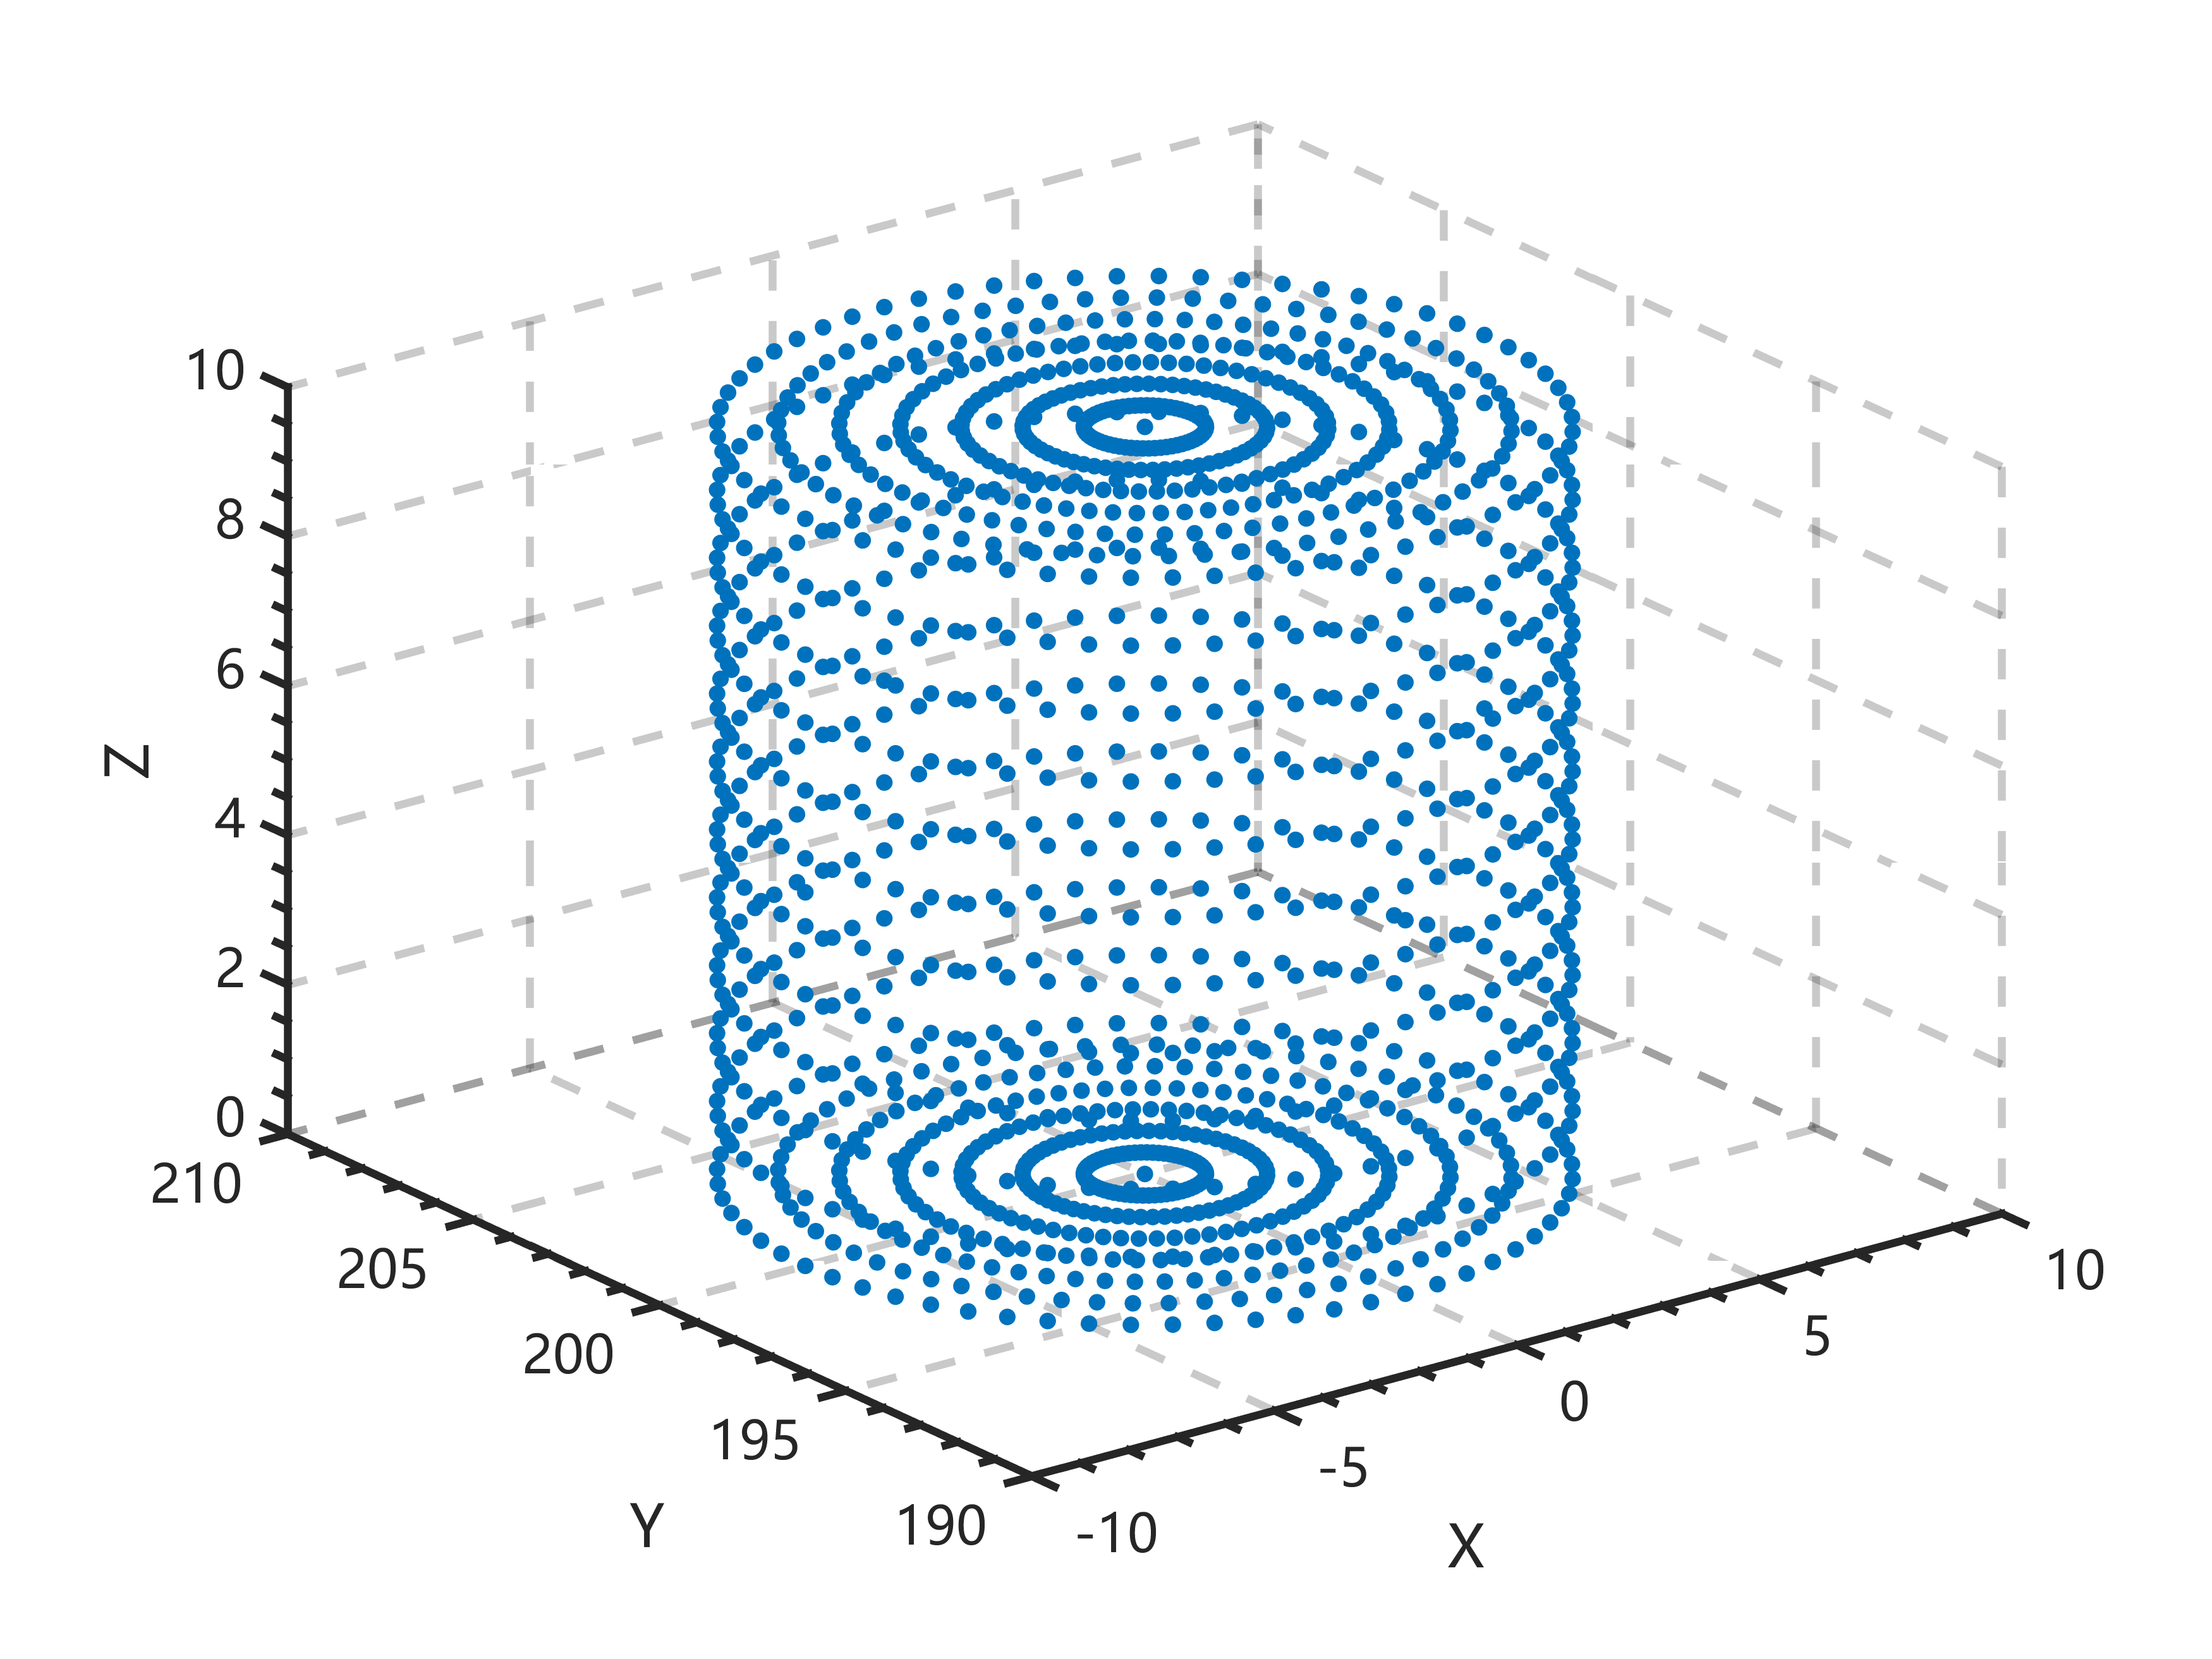
\includegraphics[width=0.5\textwidth]{圆柱体表面采样点分布.png}
    \caption{真目标表面取采样点}
     \label{fig:真目标上取采样点}
    \end{figure}
    \item 算法优化：采用粒子群-差分进化融合算法（PSO-DE）$^\text{\cite{ref10}}$，以实现全局最优解的求解。
\end{enumerate}

以这两项优化措施为基础，我们的总体思路为：
先使用粒子群算法（PSO）完成全局探索，再使用差分优化配合进行局部探索，既能防止算法过早陷入局部最优，又能加快搜索的收敛速度。

同时不断调整初始参数并进行多次迭代得到在时间网格化下的最优解，最终再结合第一问中使用过的二分法确定每枚烟幕干扰弹的精确遮蔽时间区间$\Delta T$，取区间并集后得到总遮蔽区间$T_{total}$，进而计算总遮蔽时长。根据以上分析，PSO-DE对于该模型的求解混合算法使用步骤如下：
\paragraph{Step 1 适应度函数}
依前文所述，设定适应度函数$Fitness(\mathbf{x})=T_{cov}$。
\paragraph{Step 2 决策变量归一化处理}
为了给搜索空间设置边界并合理简化问题求解，我们将8个决策变量依据题目实际要求设置边界范围，进而引入$x_i\in [0,1](i=1,2,...8)$将这8个决策变量归一化。

需要详细说明的是三枚烟幕干扰弹的投放时间$t_1,t_2,t_3$向$x_1,x_2,x_3$的归一化代换，由题目条件计算可知，导弹M1到达原点的时间为67.0s，故第三枚干扰弹的投放时间一定要在67s之前，再加上干扰弹下降到z=0至少需要19.2s，故可设定第三枚干扰弹的投放时间$t_3\leq 50s$。由于导弹投放间隔为1s，故第二枚导弹的投放时间$t_2\leq 49s$，再结合问题二得到的结果，即FY1在只投放一枚烟幕干扰弹的情况下，最佳投放时间小于0.1s，故可设定$t_1\leq 1s$。

我们设定了8个决策变量的边界值，接下来用一维仿射映射 $f(u; a, b) = a + (b - a)u$（$u \in [0,1] \implies f \in [a, b]$ 且单调）把不等式约束写进上下界；因此所有粒子永不出界、无需设置罚函数来惩罚超出边界的粒子。
具体变量代换方程如下：
\begin{equation}
    \begin{aligned}
        \begin{cases}
            \phi  = 2\pi x_1 \\
    v = 70 + 70 x_2 \\
    t_1 = x_3\\
    t_2 = t_1 + 1 + (49 - (t_1 + 1))x_4 \\
    t_3 = t_2 + 1 + (50 - (t_2 + 1))x_5 \\
    \tau_i = 20 x_{5+i}\,(i=1,2,3)
        \end{cases}    
\end{aligned}
\end{equation}    

至此，我们将决策向量转化为了一个8维归一化向量$\mathbf{x}\in [0,1]^8$。

\paragraph{Step 3 种群初始化}
在$[0,1]^8$内均匀采样 $NP$ 个粒子并设定初始速度$\mathbf{v}=\mathbf{0}$。按Step2归一化处理决策变量，用 Step1评估模型结果，得出初始个体最优解 $\mathbf{P}$ 与全局最优解 $\mathbf{G}$。
\paragraph{Step 4 种群进化}
和问题二中的$\lceil$\textbf{Step4 群体进化}$\rfloor $类似，使用粒子群算法，在每轮迭代后更新$\mathbf{P,G}$。
\paragraph{Step 5 DE优化}

目标是在保留种群多样性的同时，沿着从当前个体到全局最优的方向做出微调，加速收敛并避免 PSO 陷入局部最优解。

\noindent \textbf{1） 精英集选择}
\begin{itemize}
    \item 以适应度降序取前 $r \cdot NP$ 个体为精英集 $\mathcal{E}$。
\end{itemize}


\noindent \textbf{2） 变异}
\begin{itemize}
    \item 对每个精英 $\mathbf{x} \in \mathcal{E}$: 从全体索引集合随机无放回采样 $r_1 \neq r_2 \neq i$，构造
    \begin{equation}
        \mathbf{v}_{\text{DE}} = \mathbf{x} + F \left( \mathbf{G} - \mathbf{x} \right) + F \left( \mathbf{x}_{r_1} - \mathbf{x}_{r_2} \right)
    \end{equation}
\end{itemize}
其中变异系数$F =0.6$。

\noindent \textbf{3） 交叉}
    \begin{equation}
        u_j = 
    \begin{cases} 
    v_{\text{DE}, j}, & \text{若 } \text{rand}(0,1) \leq CR \text{ 或 } j = j_{\text{rand}} \\
    x_j, & \text{其他}
    \end{cases} 
    \end{equation}
其中j是维序数，如$v_{\text{DE}, j}$的含义为$\mathbf{v}_{\text{DE}}$的第j维；交叉率$CR \in [0.3, 0.9]$，$j_{\text{rand}}$ 是1-8中的随机整数。

\noindent \textbf{4） 数据更新}
\begin{itemize}
    \item 若 $Fitness(\mathbf{u}) > Fitness(\mathbf{x})$，则用 $\mathbf{u}$ 替换 $\mathbf{x}$: 更新群体位置和对应的个体最优解$\mathbf{P}$，并在必要时刷新 $\mathbf{G}$。
\end{itemize}

\paragraph{Step6 跳出局部峰值}
每隔 K 代将当前最差 $\rho \cdot NP$个个体（本模型求解时取$\rho= 0.2$）在$[0,1]^8$中随机重置，获得新样本并评估，其余个体仍保留更优解，通过此重置方法可以打破停滞。

\paragraph{Step7 模型微调与最优化策略生成}
迭代次数达到上限后，根据$\mathbf{G}$得到初步时间网格化下单枚导弹的粗略的遮蔽区间，此时再使用二分法，得到更为精确的遮蔽区间$\Delta T_i$，通过求并集进而得到三枚导弹的有效遮蔽时长$T_{cov}$。

\begin{figure}[htbp]
    \centering
    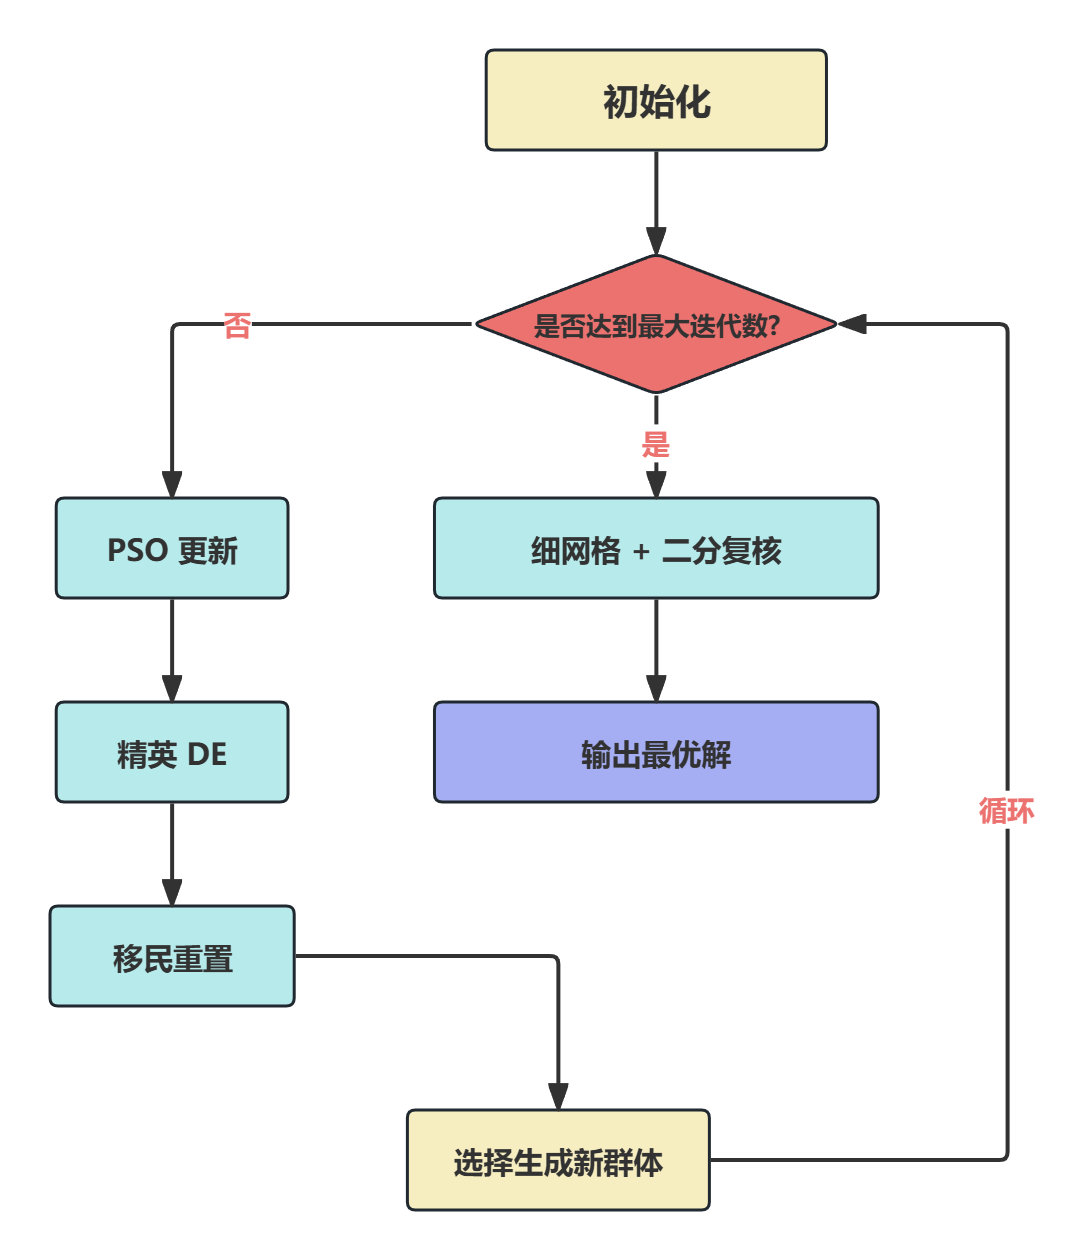
\includegraphics[width=0.5\textwidth]{PSO-DE流程图.png}
    \caption{问题三求解流程图}
    \label{问题三求解流程图}
\end{figure}
\subsubsection{模型的求解与结果分析}
根据前文的求解方法，我们可以计算得到烟幕干扰弹的投放策略，部分结果展示如表\ref{tab:smoke_bomb_detail}所示，具体精确结果已填进表格文件result1.xlsx。
\begin{table}[htbp]
  \centering
  \caption{问题三结果表}
  \begin{tabular}{cccc}
    \toprule
       \addlinespace[-2pt]
    烟幕干扰弹编号 & 
    干扰弹投放点坐标(m) & 
    干扰弹起爆点坐标(m) & 
    有效干扰时长(s) \\
       \addlinespace[-2pt]
    \midrule
       \addlinespace[-2pt]
    1 & (17800,0,1800)     & (17800,0,1800)      & 2.5 \\
       \addlinespace[-2pt]
    2 & (17914,15,1800)     & (17914,15,1800)      & 4.1 \\
       \addlinespace[-2pt]
    3 &\multicolumn{2}{c}{ 无需投放}  & 0 \\
       \addlinespace[-2pt]
    \bottomrule
  \end{tabular}
  \label{tab:smoke_bomb_detail}
\end{table}

无人机FY1的飞行方向为$7.496^\circ$,飞行速度为114.9m/s。

通过对求解结果的分析，我们可以得出以下规律：
无人机的飞行方向与x轴正向的夹角较小，由问题二的结果分析可知，这是因为因为真目标位置接近原点，故为了有效遮蔽，无人机的飞行角度一定较小。    

如图\ref{三枚烟幕干扰弹的有效遮蔽时间}所示，FY1投出的三枚烟幕干扰弹，只有前两枚能够对导弹M1起到有效遮蔽作用，且第一枚在无人机刚起飞时就进行了投放并立刻起爆成烟幕云团，紧接着第二枚在无人机飞行1s时进行投放且也在投放瞬间立刻起爆形成烟幕云团。我们随即对该现象进行了理论分析和计算验证。
\begin{figure}[htbp]
    \centering
   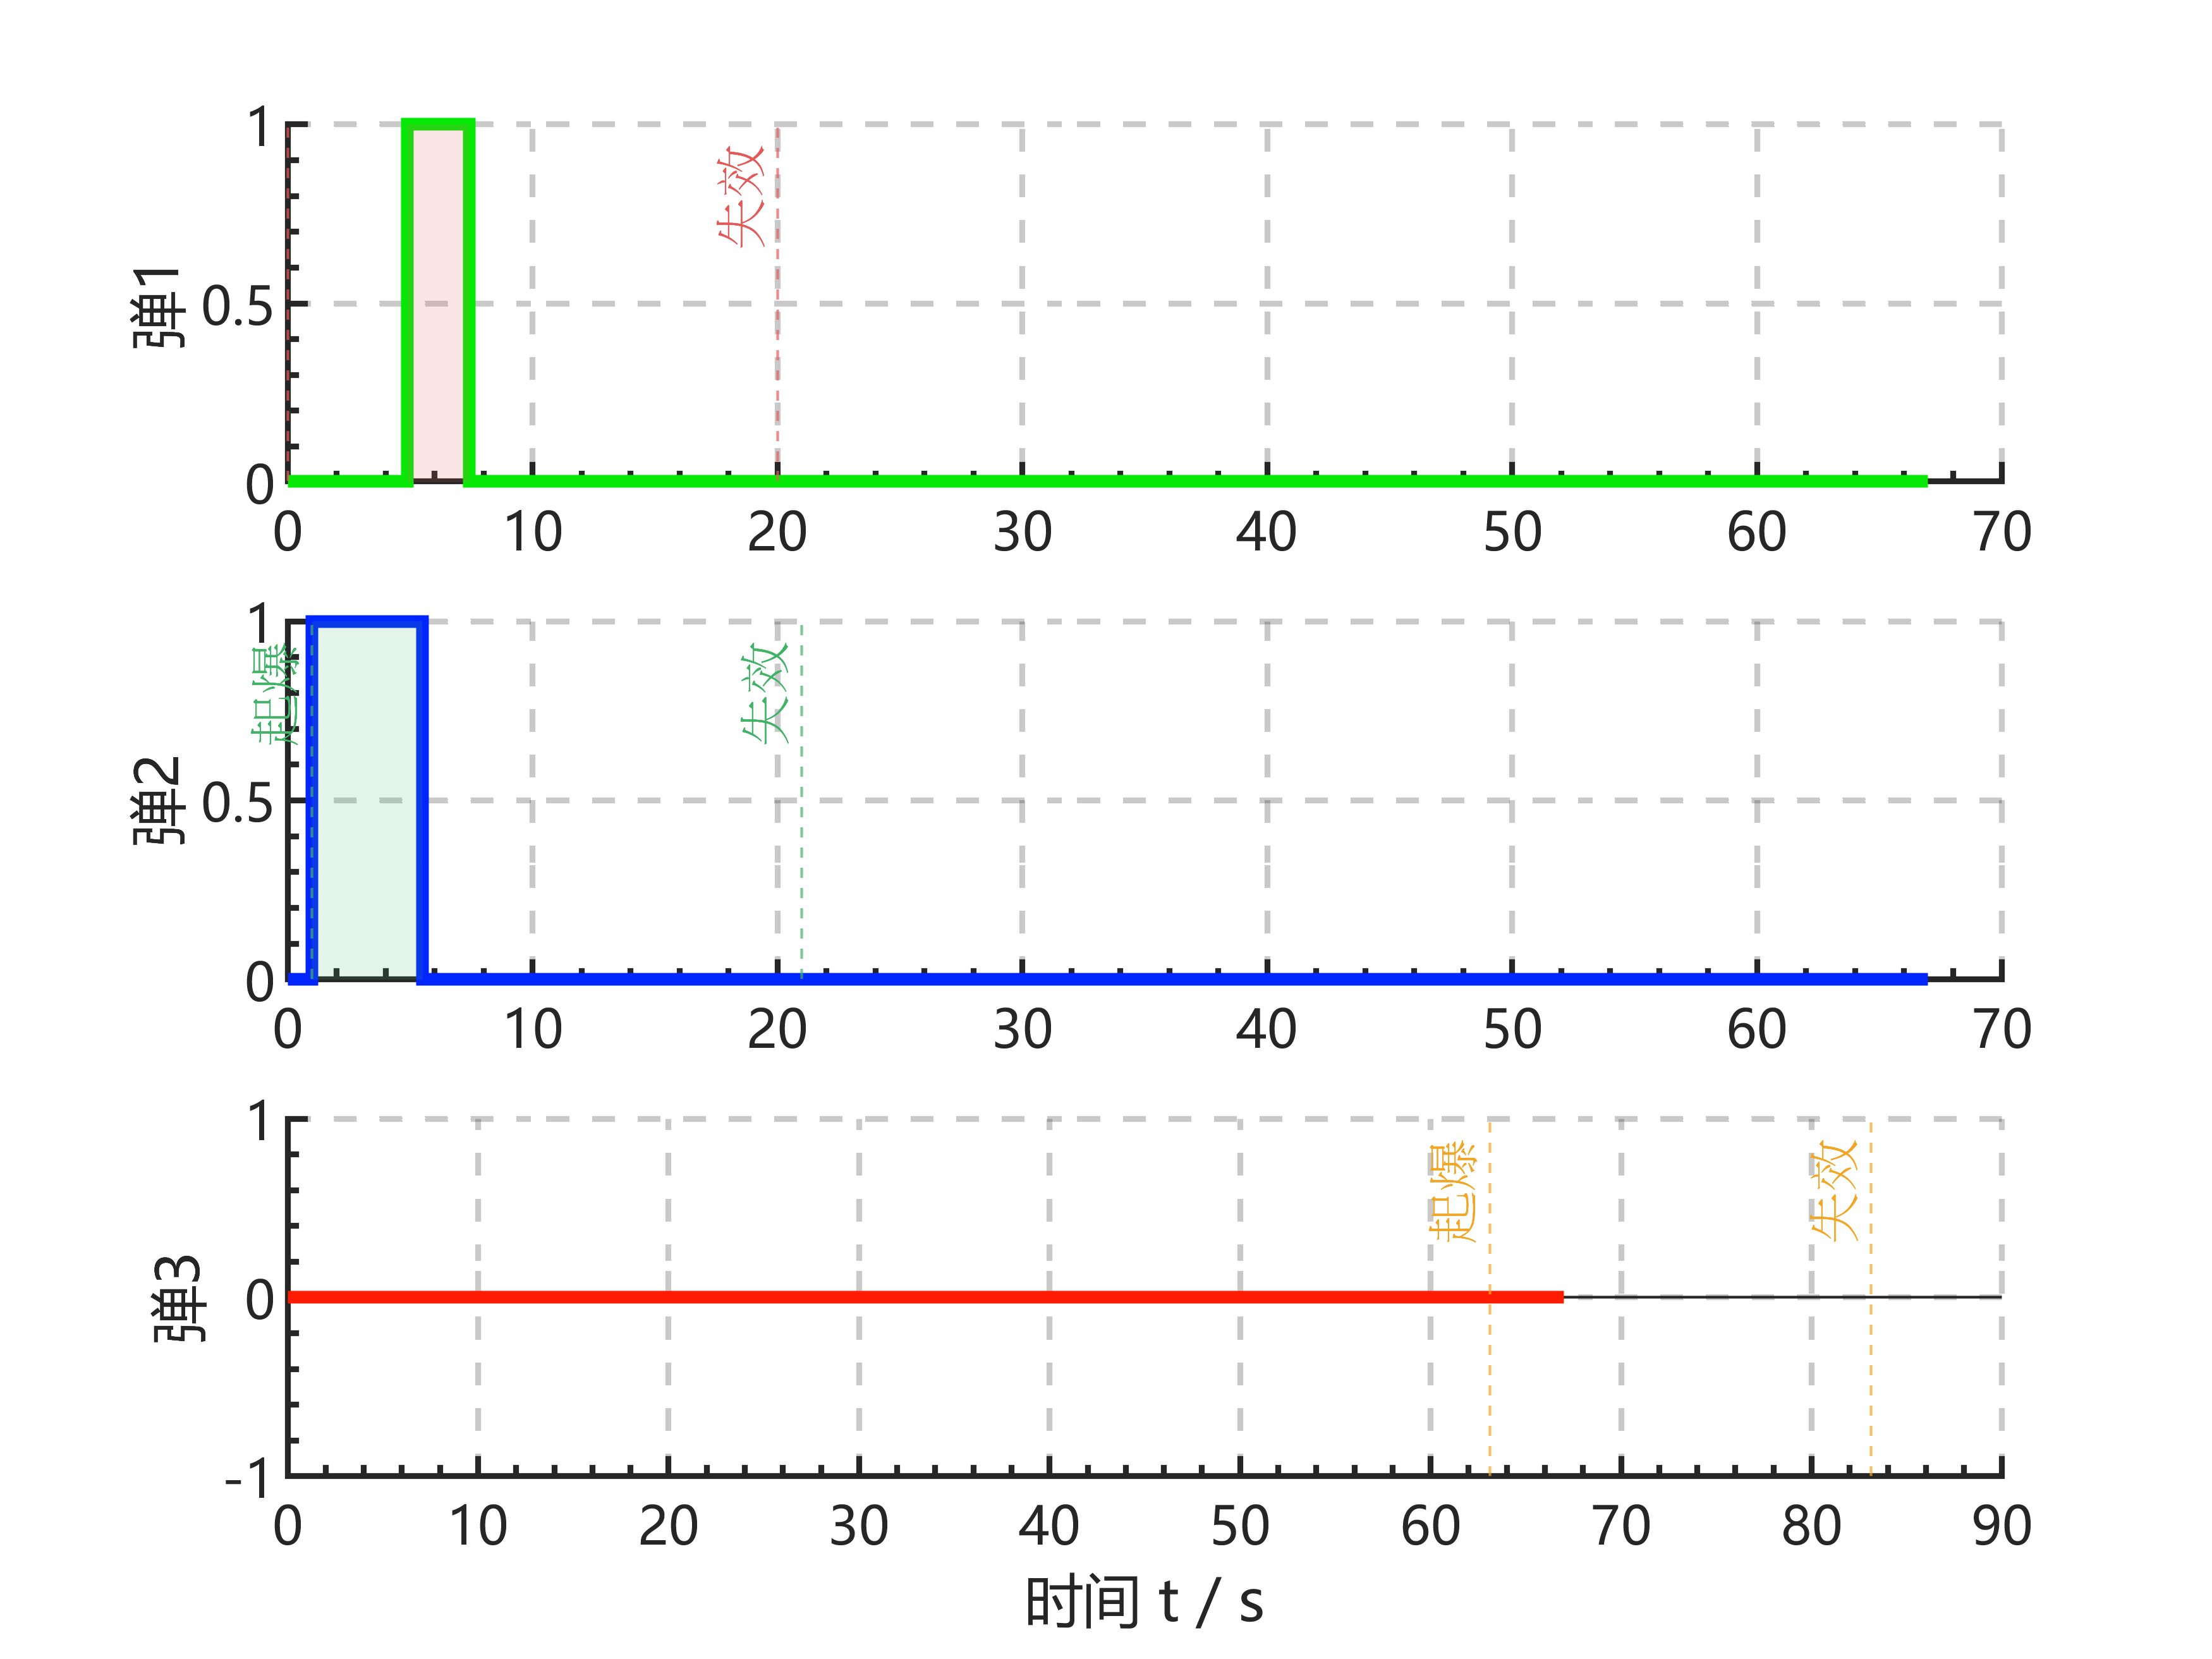
\includegraphics[width=0.6\textwidth]{三枚弹各自“完全遮蔽”时间线.png}
    \caption{FY1投出的三枚烟幕干扰弹的有效遮蔽时间}
    \label{三枚烟幕干扰弹的有效遮蔽时间}
\end{figure}

在FY1的飞行方向为$7.496^\circ$,飞行速度为114.9m/s的假设下，容易计算出，导弹M1约在第6s时和无人机FY1大致相遇并迅速和FY1拉开越来越大的距离。FY1即使在2s时就投放第三枚烟幕干扰弹（此时第二枚云团在发挥遮蔽作用），干扰弹的投出位置的x坐标约为18000，而此时导弹M1所到达位置的x坐标约为19400,M1约4.5s后即第6.5s时经过烟幕弹抛出位置，从图\ref{三枚烟幕干扰弹的有效遮蔽时间}上可以看出，整个过程都有云团在发挥遮蔽作用，而当第一枚云团的遮蔽效果结束时，导弹早已飞出第三枚云团的有效遮蔽范围。因此验证了求解结果中烟幕弹投放策略的合理性。


\subsection{问题四模型的建立与求解}
\begin{figure}[htbp]
    \centering
    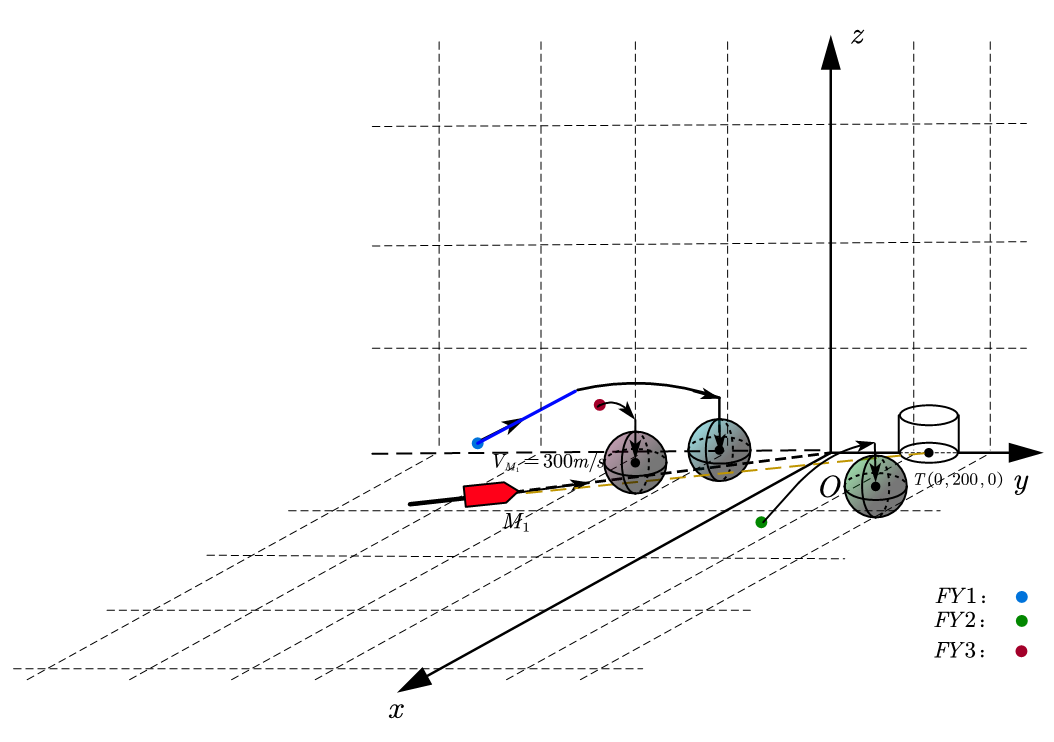
\includegraphics[width=0.5\textwidth]{FY1、FY2、FY3投放烟幕干扰弹的运动轨迹示意图.png}
    \caption{无人机投放烟幕干扰弹示意图 }
    \label{}
\end{figure}
参考FY1,FY2,FY3-M1-烟幕云团的位置示意图可建立以下模型：
\subsubsection{模型的建立}
相较于问题二和问题三，问题四从单机FY1投放烟幕干扰弹干扰M1变成FY1、FY2、FY3多机协同以实现遮蔽时间互补，决策变量的维度为12，分别为三台无人机的飞行速度$v_1,v_2,v_3$，飞行方向$\phi_1,\phi_2,\phi_3 $,三枚烟幕干扰弹的投放时间$t_{1,1},t_{2,1},t_{3,1}$和从投放到起爆的间隔时间$\tau_1,\tau_2, \tau_3 $。
\subsubsection{模型的求解与结果分析}
由于模型变量维数较高，我们基于第二问所建立的模型，采用这样一种策略来简化计算量：先求出每个无人机单独投放烟幕干扰弹的最佳情况，再以此参数为基准，不断调整整个粒子群的空间，确保初始粒子能落在全局最优解的附近，防止一开始的初始位置就落在局部峰值附近，使收敛过早地结束，陷入局部最优解中。对于这个模型的求解，我们仍使用PSO-DE算法，前期先进行全局搜索、实现快速收敛，同时利用DE 的定向扰动与自适应步长来增强跨盆地跳跃和精确找到最优解的能力，从而降低陷入局
部最优解的风险，提升复杂问题上的处理能力。最终来确定烟幕干扰弹投放的最优策略。最终求出结果部分展示见下表，完整且更为精确的结果已填入附件result2.xlsx中。
\begin{table}[htbp]
  \centering
  \caption{无人机烟幕干扰弹投放策略}
  \begin{tabular}{cccccc}
    \toprule
    
    无人机编号 & 速度 (m/s) & 干扰弹投放点坐标 (m) & 干扰弹引爆点坐标 (m) & 遮蔽时长 (s) \\

    \midrule

    FY1  & 70 & (17940, 7, 1800) & (17940, 7, 1800) & 4.62 \\

    FY2  & 133 & (12920, 379, 1400) & (13246, 16, 1334) & 3.96 \\

    FY3  & 119 & (6091, -383, 700) & (6108, 92, 621.520) & 4.78 \\
 
    \bottomrule
  \end{tabular}
  \label{tab:drone_smoke_interference}
\end{table}

图\ref{FY1，FY2，FY3遮蔽时间线}和图\ref{FY1，FY2，FY3投放干扰弹空间展示}详细又直观地展示了FY1,FY2,FY3所投放出的三枚烟幕干扰弹在时间轴上和三维空间中对M1的遮蔽作用。
\begin{figure}[htbp]
    \centering
   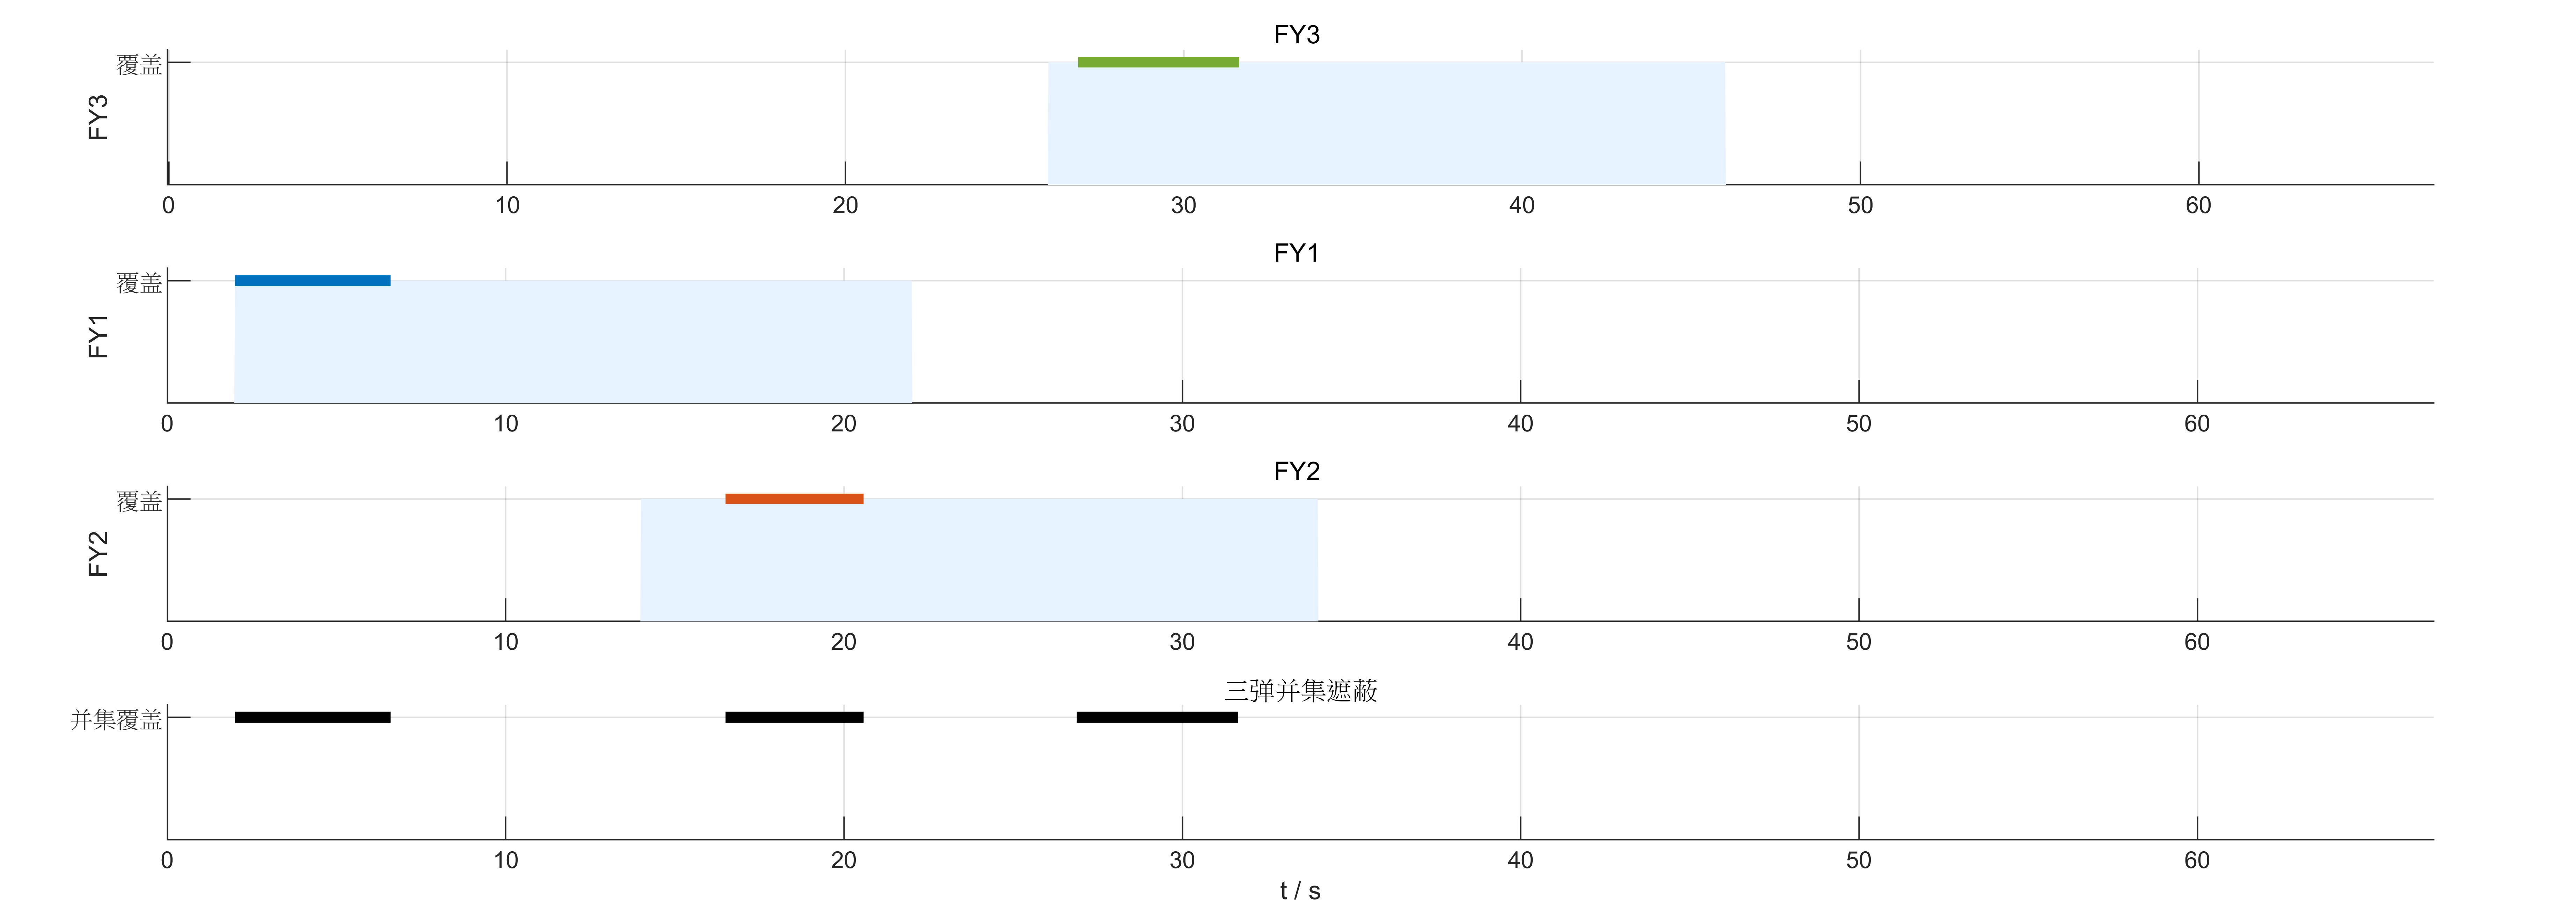
\includegraphics[width=0.8\textwidth]{FY1，FY2，FY3遮蔽时间.png}
    \caption{FY1，FY2，FY3遮蔽时间线 }
    \label{FY1，FY2，FY3遮蔽时间线}
\end{figure}

\begin{figure}[htbp]
    \centering
   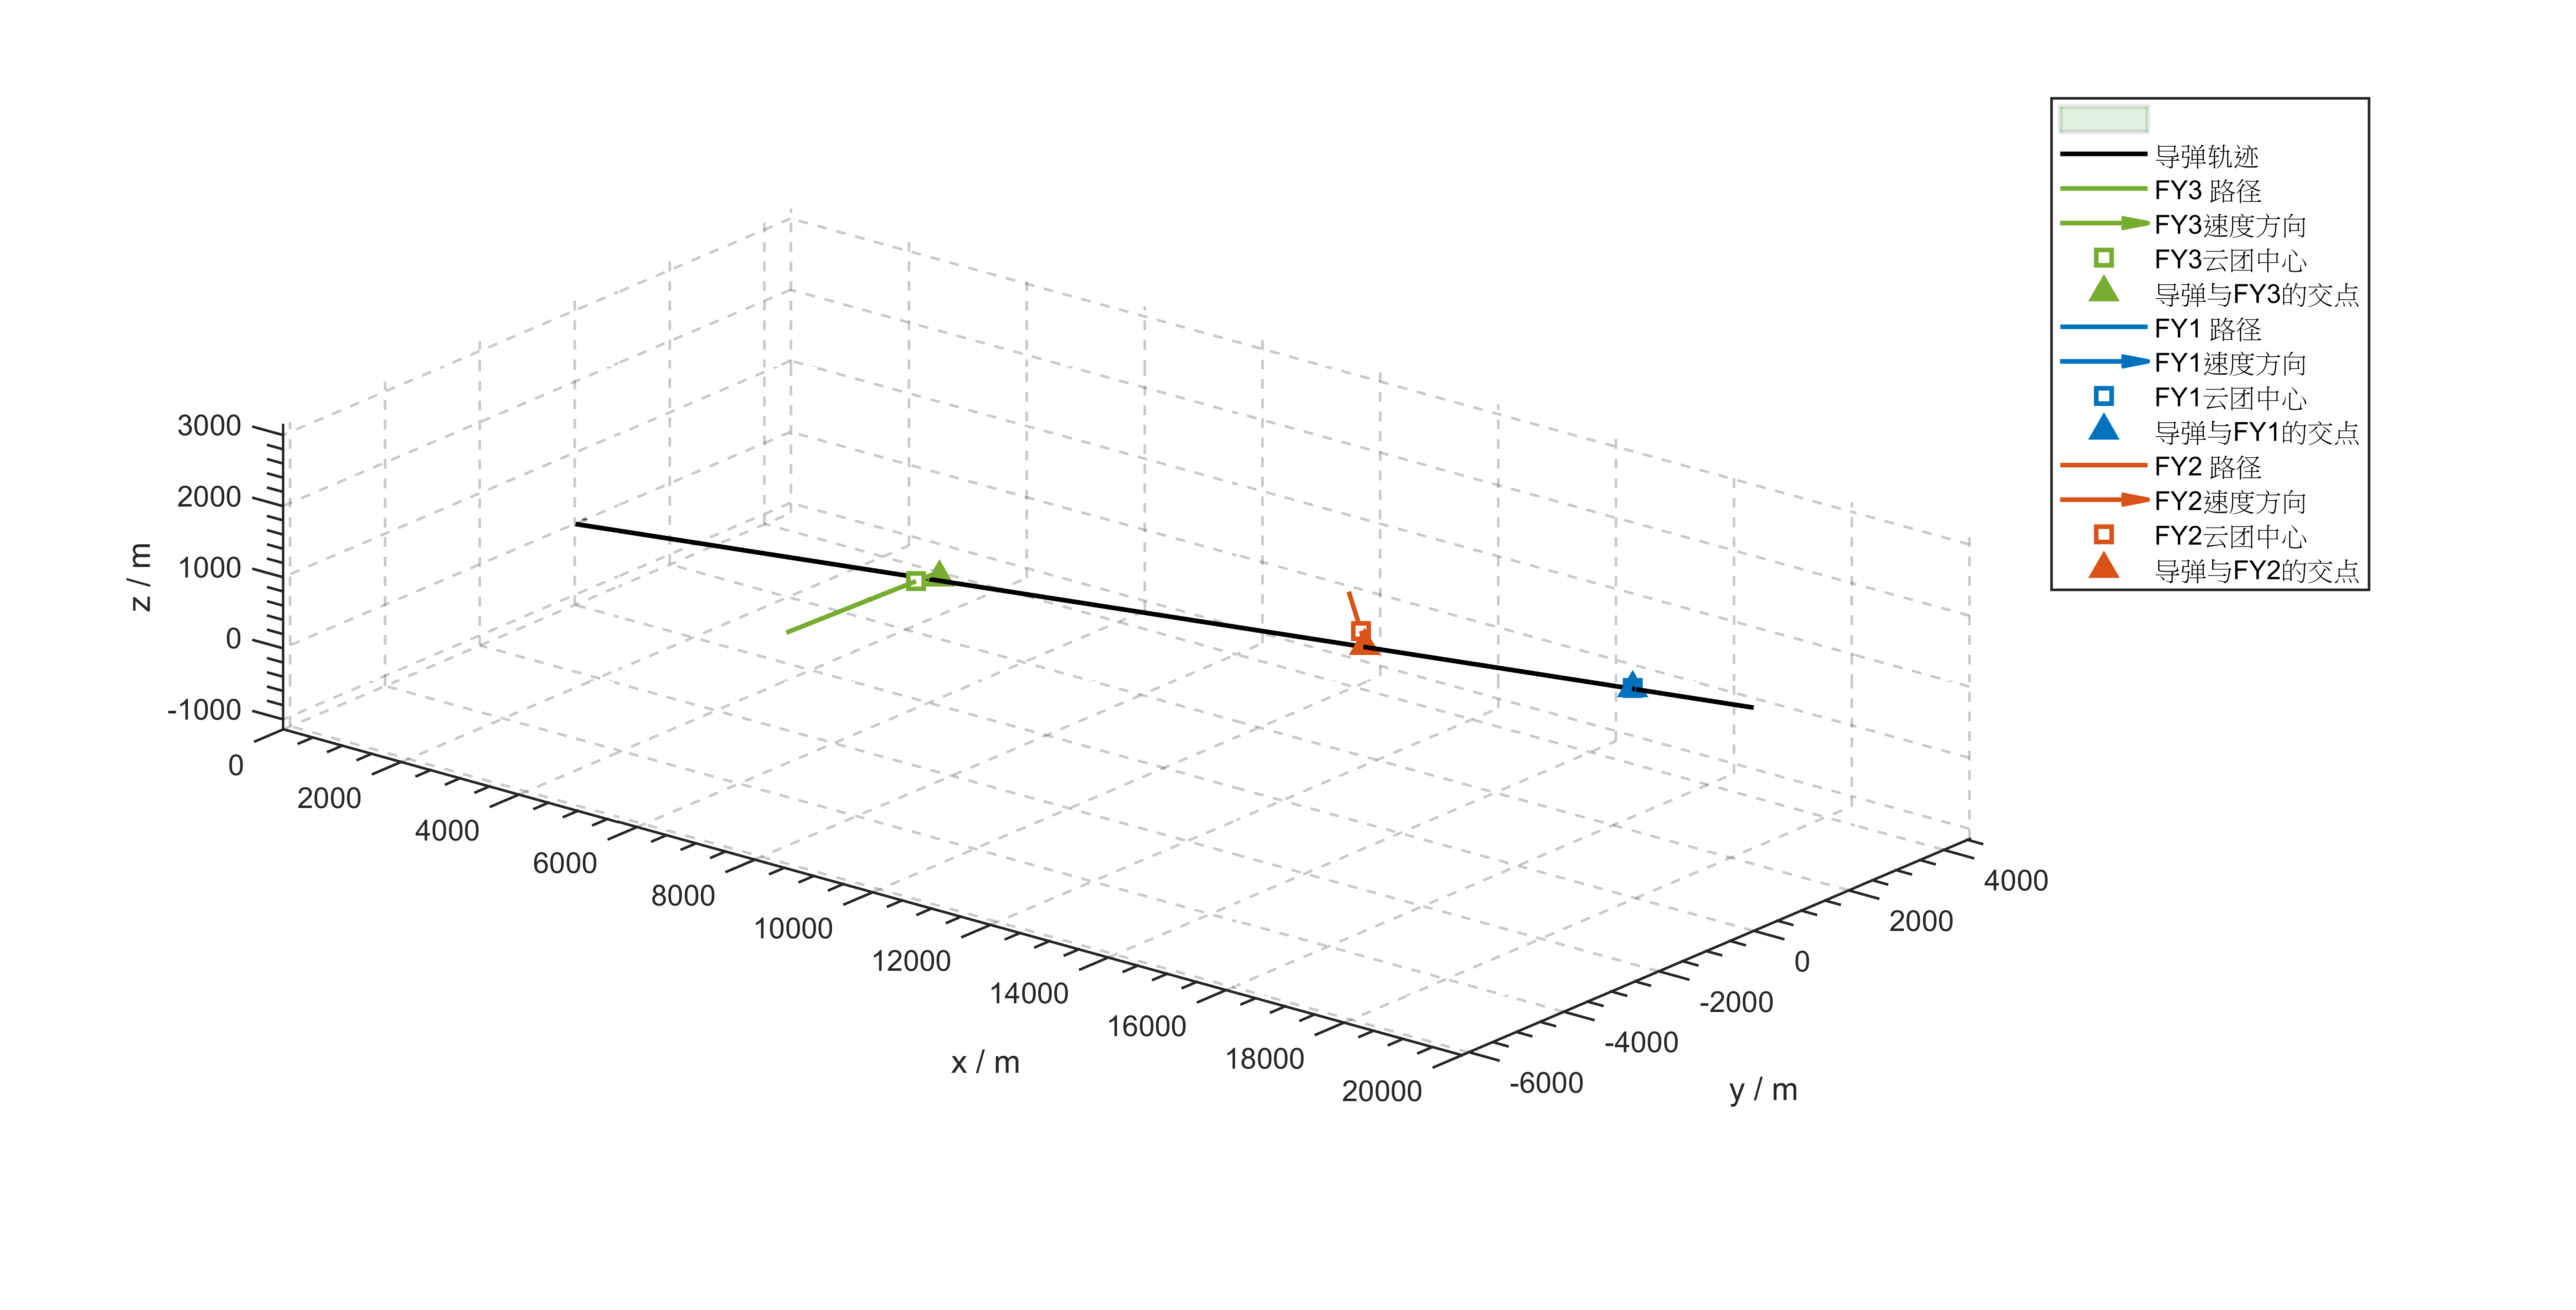
\includegraphics[width=0.8\textwidth]{FY1，FY2，FY3投放烟幕干扰弹轨迹与M1运动轨迹图.png}
    \caption{FY1，FY2，FY3投放干扰弹空间展示 }
    \label{FY1，FY2，FY3投放干扰弹空间展示}
\end{figure}
\newpage
分析以上结果，我们可以得到以下规律：
\begin{itemize}
    \item FY1，FY2，FY3的飞行方向都趋向于M1的运动轨迹，甚至近似垂直，即无人机都争取最快赶到导弹和真实目标点之间，并立刻投放烟幕干扰弹。这与问题二、三中总结的规律相符，验证了规律和结果的合理性。
    \item FY1的遮蔽时间是4.62s，略低于问题二的求解结果4.64s，这可能是因为求解时受限于迭代次数，但该误差属于可接受范围，也验证了问题二和问题四结果的合理性。
\end{itemize}
\subsection{问题五模型的建立与求解}
FY(1-5)-M(1-3)-烟幕云团的位置示意图如下页图15所示。
\newpage
\begin{figure}[htbp]
    \centering
    \label{}
   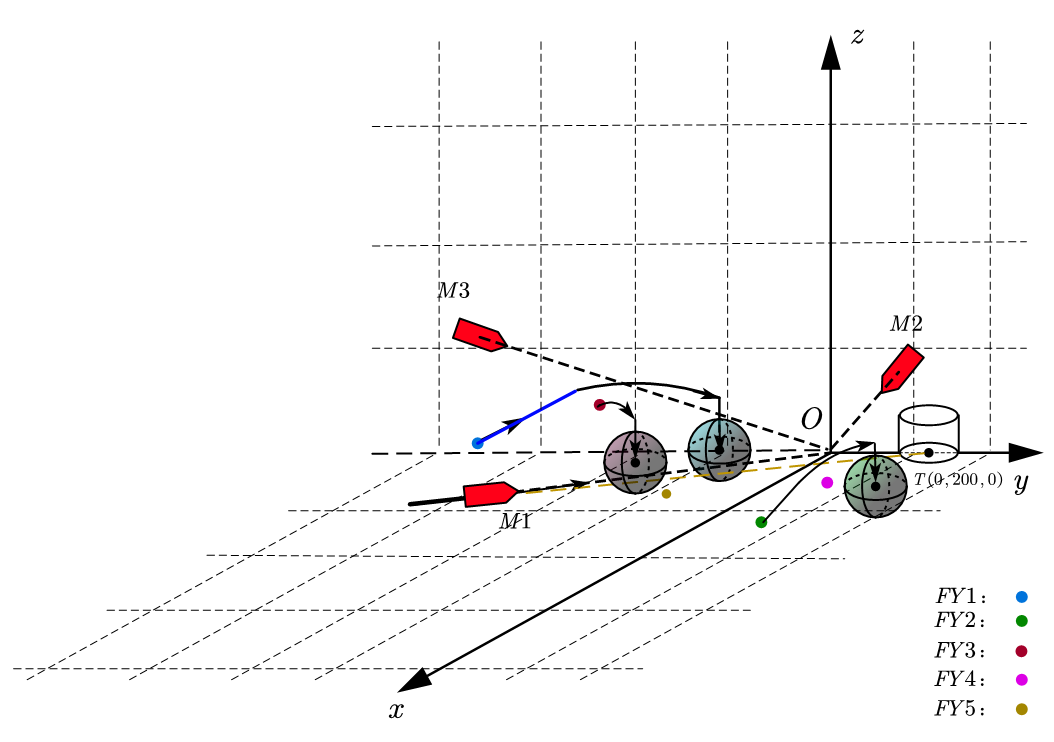
\includegraphics[width=0.5\textwidth]{FY1到FY5投放烟幕干扰弹的运动轨迹图.png}
    \caption{无人机投放烟幕干扰弹示意图 }
\end{figure}


\subsubsection{模型的建立}
对于该问题，我们认为，同一时刻允许不同云团分别遮挡不同连线，只要至少一朵云团中心到所有连线的距离在10m内即可。该问题所建立的模型整体上与前面问题所建立的模型相似，但决策变量过多，为40维。为了简化模型，我们将该问题分解为两个子问题。

\textbf{1.任务分配模型}

为了最大化总遮蔽时间，我们设定每个导弹都至少被一架无人机干扰，且一个无人机只负责遮蔽一个导弹。由无人机个数和导弹个数可知这是一个非标准形式的指派问题。分析前面问题的求解结果，我们发现，干扰弹几乎都尽可能在前期投放和起爆，这直接说明了导弹离原点距离越远时，烟幕云团的遮蔽效果越好。所以为了使整体上无人机群对导弹的干扰程度最大，我们以分配后无人机与各自负责干扰的导弹距离之和为判断依据，距离越短，越能尽早投放干扰弹，干扰效果越好。

\textbf{2.分组策略优化模型}

待任务分配模型解决后，就将该问题分解为了三个类似于问题三、问题四的独立的多个模型。通过对分解后的多个模型分别进行求解，可以得到最终遮蔽总时长$T_{cov}$。

\subsubsection{匈牙利解法在模型求解中的运用}
对于任务分配模型这个指派问题的求解，我们采用经典的匈牙利解法$^\text{\cite{ref6}}$。
\paragraph{Step1 距离矩阵}
行对应FY1到FY5；列对应M1到M3，表中数据是对应的距离（单位：$\times 10^4$米）
\[
D = \begin{bmatrix}
740 & 189 & 41 \\
6032 & 5013 & 3949 \\
20689 & 18392 & 15120 \\
8504 & 6605 & 5577 \\
5589 & 4600 & 2732 \\
\end{bmatrix}
\]

\paragraph{Step2 转成标准指派问题}
增添两列M3，得如下$5\times 5$矩阵，将模型转化为标准指派问题。
\[
C = \begin{bmatrix}
740 & 189 & 41 & 41 & 41 \\
6032 & 5013 & 3949 & 3949 & 3949 \\
20689 & 18392 & 15120 & 15120 & 15120 \\
8504 & 6605 & 5577 & 5577 & 5577 \\
5589 & 4600 & 2732 & 2732 & 2732 \\
\end{bmatrix}
\]

\paragraph{Step3 匈牙利算法}
\begin{enumerate}
\item[1)] 每行减行最小值 \(\{41, 3949, 15120, 5577, 2732\}\)，得
\[
\begin{bmatrix}
699 & 148 & 0 & 0 & 0 \\
2083 & 1064 & 0 & 0 & 0 \\
5569 & 3272 & 0 & 0 & 0 \\
2927 & 1028 & 0 & 0 & 0 \\
2857 & 1868 & 0 & 0 & 0 \\
\end{bmatrix}
\]

\item[2)] 每列减列最小值 \(\{699, 148, 0, 0, 0\}\)，得
\[
R = \begin{bmatrix}
0 & 0 & 0 & 0 & 0 \\
1984 & 916 & 0 & 0 & 0 \\
4870 & 3124 & 0 & 0 & 0 \\
2228 & 880 & 0 & 0 & 0 \\
2158 & 1720 & 0 & 0 & 0 \\
\end{bmatrix}
\]

\item[3)] 选择独立零元素：\((1,1)\)、\((4,2)\)、\((2,3)\)、\((3,4)\)、\((5,5)\)，此时独立零元素已有5个，则表示已可确定最优指派方案，此时令矩阵中独立零元素为1，其他元素为0，可得最优解矩阵为
\[
\begin{bmatrix}
1 & 0 & 0 & 0 & 0 \\
0 & 0 & 1 & 0 & 0 \\
0 & 0 & 0 & 1 & 0 \\
0 & 1 & 0 & 0 & 0 \\
0 & 0 & 0 & 0 & 1 \\
\end{bmatrix}
\]
\item[4)] 读出指派：
\begin{itemize}
\item \((1,1)\) → FY1 指派到 M1
\item \((4,2)\) → FY4 指派到 M2
\item \((2,3)\)、\((3,4)\)、\((5,5)\) → FY2/FY3/FY5 指派到 M3
\end{itemize}
得5×3指派矩阵：
\[
X = \begin{bmatrix}
1 & 0 & 0 \\
0 & 0 & 1 \\
0 & 0 & 1 \\
0 & 1 & 0 \\
0 & 0 & 1 \\
\end{bmatrix}
\]
\end{enumerate}

这个指派矩阵将每个无人机分配到了一个导弹线路。此时我们可以构建起每个无人机的投弹策略模型，再按照问题三中所阐述的求解思路，使用PSO-DE优化算法求解此模型。
\subsubsection{模型的求解与结果分析}
根据以上分析，求解出投放策略部分。本文将无人机扩展为FY1的飞行和投弹策略展示在表6中，完整结果已填入表格文件result3.xlsx中。
\begin{table}[htbp]
\centering
\caption{无人机相关数据}
\begin{tabular}{@{}llllll@{}}
\toprule
 无人机运动方向 & 速度 (m/s)  & 投放点坐标 (m) & 起爆点坐标 (m) & 干扰时长 (s) \\
\midrule
 182.2 & 82.2 & （17767.3,-1.2,1800） &  （17746.1,-2.11,1799.6）  & 4.3 \\
182.2 & 82.2 & （17556.2,-10.1,1800） &  （17281.2,-21.2,1745.3）  & 3.0 \\
182.2 & 82.2 & （17087.2,-29.3,1800） &  （16727.9,-44.3,1705） & 2.0\\
\bottomrule
\end{tabular}
\end{table}

图16展示了三枚导弹M1,M2,M3被遮蔽的时长。
\begin{figure}[htbp]
    \centering
   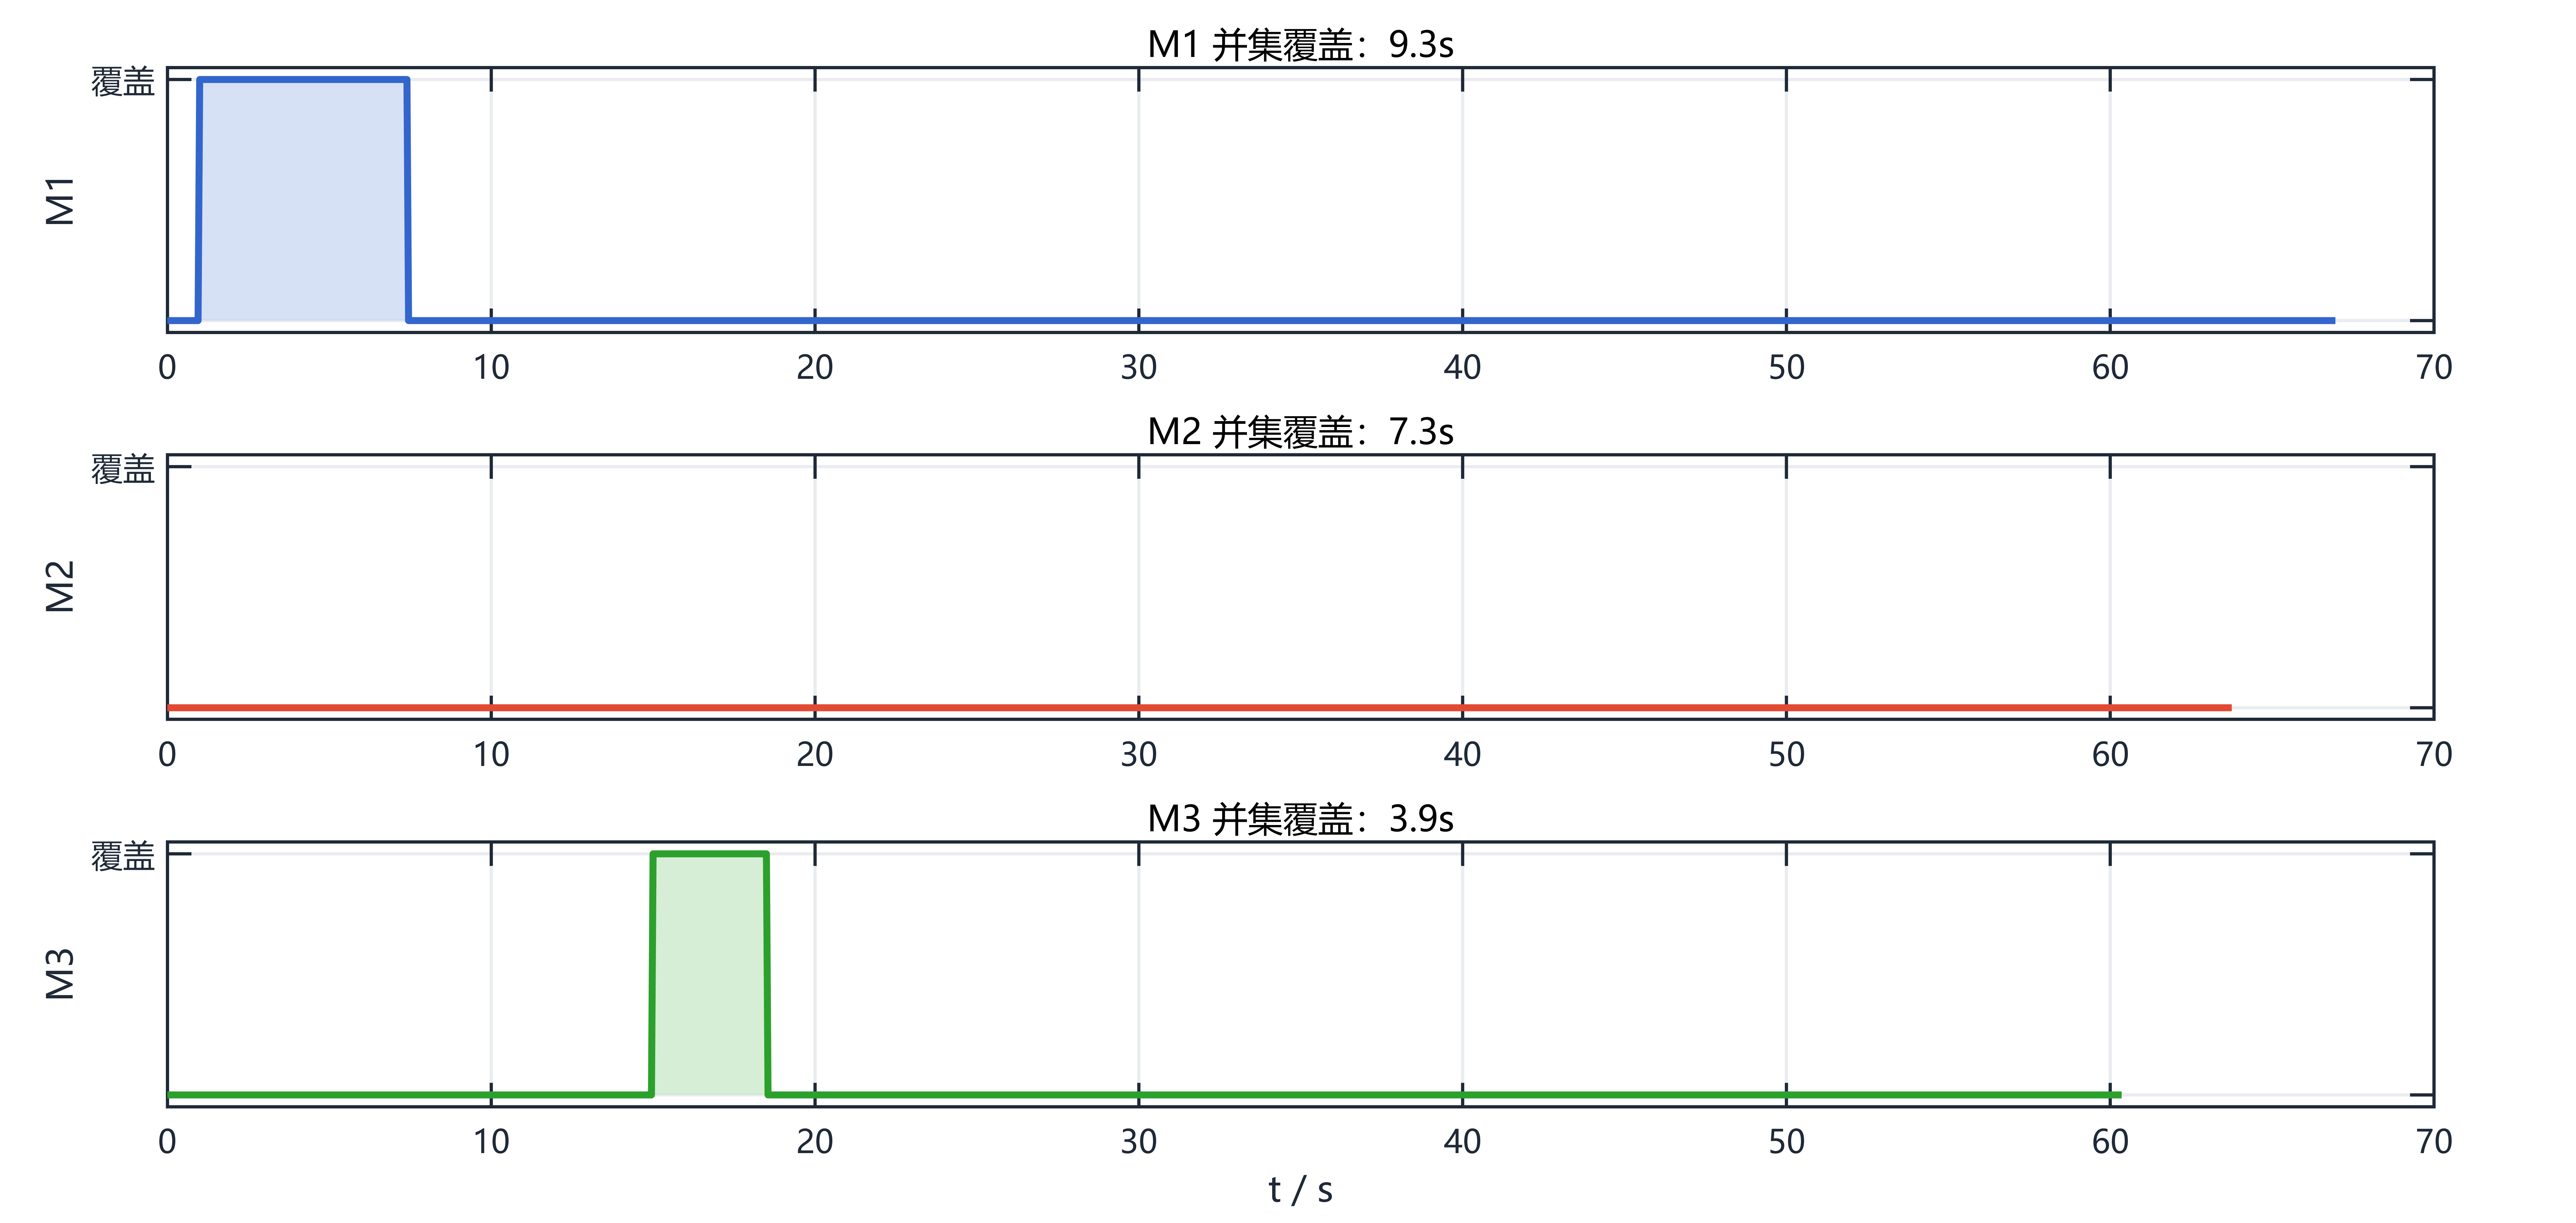
\includegraphics[width=0.8\textwidth]{对M1，M2，M3的遮蔽时长.png}
    \caption{M1，M2，M3的遮蔽时长 }
    \label{M1，M2，M3的遮蔽时长}
\end{figure}
\newpage
对以上结果分析可知，总遮蔽时长$T_{cov}=20.5s$。结合前四个问题可知，此结果较为可靠。


\section{模型评价与推广}
\subsection{优点}
\begin{itemize}
    \item 合理地分析了几何模型，确定了最关键的遮蔽判据。
    \item 在PSO算法的基础上采用了PSO-DE，防止过早地陷入局部最优解。
    \item 简化问题五，将其分解为两个子问题。先利用匈牙利算法解决任务分配问题，从而以问题三和问题四为基础解决问题五。
\end{itemize}
\subsection{缺点}
问题四需要不断的调整参数，且需要较大的迭代次数，否则仍容易陷入局部最优。
\subsection{推广}
本文所制定的烟幕干扰弹投放策略，可推广至多个无人机对多个导弹的联合干扰优化模型，可为军事上无人机投放烟幕干扰弹提供策略。
\begin{thebibliography}{99}
\bibitem{ref1}
DeepSeek, DeepSeek-R1-0528, 深度求索（DeepSeek）, 2025-09-05

\bibitem{ref2}
ChatGPT, ChatGPT 5Thinking,OpenAI,2025-09-05

\bibitem{ref3}
豆包AI助手, 2025通用版, 北京字节跳动科技有限公司, 2025-09-05

\bibitem{ref4}
杨冬英,邱选兵,李传亮,等.烟雾干扰光学制导武器中Mie散射系数快速算法[J].火力与指挥控制,2017,42(08):56-60.

\bibitem{ref5} 
姜启源, 谢金星, 叶俊. 数学模型[M]. 6版. 北京: 高等教育出版社, 2024.

\bibitem{ref6} 
胡运权, 郭耀煌. 运筹学教程[M]. 5版. 北京: 清华大学出版社, 2018.

\bibitem{ref9}
李云娟,樊雪双.基于数学建模的PSO-DE算法在机器人智能拣货过程中的应用研究[J].自动化与仪器仪表,2024,(03):197-200+205.DOI:10.14016/j.cnki.1001-9227.2024.03.197.

\bibitem{ref10}
孟小丁.学习驱动的高效混合粒子群算法及应用研究[D].青海师范大学,2025.DOI:10.27778/d.cnki.gqhzy.2025.000016.

\bibitem{ref11}
朱晓东,任春晓,刘晓兰,等.基于适应度地形分析的优化算法调度方法[J/OL].郑州大学学报(工学版),1-8[2025-09-06].https://doi.org/10.13705/j.issn.1671-6833.2025.03.017.

\end{thebibliography}
\begin{appendices}
    \section{支撑材料列表}
    \begin{table}[htbp]
    \centering
    \begin{tabular}{ccc}
        \toprule
        序号 & 文件名                & 材料说明             \\
        \midrule
        1    &AI使用说明.pdf          &AI使用说明           \\
        2    & wenti\_1.m               &问题一脚本文件                    \\
        3    & wenti\_2.m              &问题二脚本文件                    \\
        4    &wenti\_3.m              &问题三脚本文件                      \\
        5    &wenti\_4.m              &问题四脚本文件                      \\
        6    &wenti\_5.m              &问题五脚本文件                      \\
        7    &refine\_mask\_with\_bisection\_.m&二分法函数                    \\
        8    &q2\_objective\_cylinder\_.m &问题二遮蔽时长计算函数                    \\
        9&objective\_cover\_time\_vec\_ .m&初步评估函数\\
        10&missile\_cloud\_events\_ .m&连线与云团中心的距离关系函数 \\
        11&mask\_one\_cover\_.m&对某一枚导弹的每个干扰弹遮蔽时间函数 \\
        12&mask\_any\_cover\_.m&所有采样点的遮蔽时间函数 \\
        13&drop\_blows\_from\_S\_.m& 无人机运动轨迹函数 \\
        14& decodeVars\_with\_gap\_ .m&FY1投放三枚干扰弹的投放函数 \\
        15&cover\_time\_point\_target\_.m&时间空间离散化函数\\
        16&cover\_time\_cylinder\_sampling\_.m&对每个采样点的遮蔽区间取交 \\
        17& cover\_one\_at\_time\_.m& 判断某一枚导弹在t时刻是否被遮挡 \\
        18&cover\_any\_at\_time\_.m& 判断导弹遮蔽函数\\
        19& cloudFullyCovers\_vec\_.m& 遮蔽判据函数 \\
        \bottomrule
    \end{tabular}
    \end{table}
    \section{问题一主程序——matlab 源程序}
    \begin{lstlisting}[language=matlab]
        clear; clc;
%设置需要使用的常量，单位是m,s
FY1=[17800, 0, 1800]; % 无人机FY1的初始位置
M1=[20000, 0, 2000];  % 导弹M1的初始位置
v_F=120;              % 规定无人机速度
v_dao=300;              % 规定导弹速度
td=1.5;               % 规定投烟雾弹的放时刻
tau=3.6;              % 规定烟雾弹空中降落时间
te=td + tau;          % 起爆时刻
vd=3;              % 设置云团匀速下落的速度
R_yun=10;             % 设置云团的有效半径
g=9.8;                % 设置重力加速度
r_R=7;                 %规定圆柱体的半径
r_z=[0, 10];         %圆柱体的高
r_xy=[0, 200];        %圆柱体的圆心

%计算FY1朝向原点的水平单位向量
d_h=-[FY1(1), FY1(2), 0];
d_h=d_h/norm(d_h);
S=FY1+v_F*td*d_h;            % 投放点S
E=S+v_F*tau*d_h+0.5*[0,0,-g]*tau^2;      %起爆点E

%在圆柱体上采样，通过采样多个点近似于整个圆柱体
n_r=30;        %在圆柱体径向的采样数
n_z=30;         %在圆柱高度向的采样数
nth=16;       %在圆柱体周向的采样数
include_b=false;        %是否包含边界点

[interval,T_total,info]=cover_time_cylinder_sampling_( ...
    M1, v_dao, E, vd, te, R_yun, r_xy, r_R, r_z, ...
    n_r, nth, n_z, include_b);

% 输出计算出的各项结果
format long g
fprintf('采样点总数:%d (n_r=%d,Nθ=%d,n_z=%d,边界=%d)\n', ...
    info.n_p, n_r, nth, n_z, include_b);

if isempty(interval)         %判断是否为0
    disp('圆柱体在任何时刻都未被完全遮蔽。');
else
    fprintf('圆柱体被完全遮蔽的时间区间（共%d段)：\n', size(interval,1));
    for k=1:size(interval,1)
        fprintf('  第%02d段: [%.9f , %.9f] s(时长=%.9f s)\n', ...
            k, interval(k,1), interval(k,2), interval(k,2)-interval(k,1));
    end
    fprintf('\n圆柱体的有效遮蔽总时长:T_all=%.9f s\n', T_total);
end
evt=missile_cloud_events_(M1, v_dao, E, te, vd, R_yun);  

fprintf('\n导弹M1与云团的相对位置关系：\n');
fprintf('云团有效的时间区间：[%.6f，%.6f] s\n', evt.t_window(1), evt.t_window(2));
if ~evt.has_intersection        %判断导弹在云团里的时间是否为0
    fprintf('导弹M1未进入云团。\n');
else
    fprintf('导弹M1进入云团时刻：t_in=%.9f s\n', evt.t_in);
    fprintf('导弹M1脱离云团时刻：t_out=%.9f s\n', evt.t_out);
    fprintf('M1在云内经历时间：Δt=%.9f s\n', evt.duration);
end

    \end{lstlisting}
    \section{问题二主程序——matlab 源程序}
    \begin{lstlisting}[language=matlab]
        %问题2：FY1无人机投放1枚烟雾干扰弹最优方案
clear;clc;

%定义需要使用的量
g=9.8;   %定义重力加速度
M1=[20000,0,2000];   %定义M1的初始位置
v_dao=300;   %定义导弹的速度
R_yun=10;   %定义云团的有效半径
v_yun=3;    %定义云团匀速下落的速度
r_R=7;          %规定圆柱体的半径
r_xy=[0,200];        %圆柱体的圆心
r_z=[0,10];      %圆柱体的高

%在圆柱体上采样，通过采样多个点近似于整个圆柱体
n_r=4;        %在圆柱体径向的采样数
n_z=4;         %在圆柱高度向的采样数
nth=16;       %在圆柱体周向的采样数
include_b=false;        %是否包含侧壁/端面边界点

% 设置决策变量边界[速度, 角度, 飞行时间, 空中下降时间]
lb=[ 70,  0,  0,  0];            %设置下界
ub=[140, 2*pi, 60, 15];        %设置上界

% 设置PSO参数
n_p=60;              % 设置粒子数
w0=0.9; w1 = 0.40;        % 设置惯性权重，采取线性递减
c1=1.49; c2 = 2;       % 设置个体与社会的学习因子
i_t=60;             % 设置算法的迭代次数

% 初始化过程
dim=4;     %四个维度
rng('shuffle');
v=zeros(n_p,dim);                % 初始化粒子的速度
x=lb+(ub-lb).*rand(n_p,dim);     % 初始化粒子的位置

%评估初值,使用循环，实现PSO最小化
fit=zeros(n_p,1);
for i=1:n_p
    fit(i)=-q2_objective_cylinder_( x(i,:),M1,v_dao,g,v_yun,R_yun, ...
        r_xy,r_R,r_z,n_r,nth,n_z,include_b );
end
Pbest=x;   PbestVal=fit;     %个体最优
[GbVal, gid]=min(fit);         % 最小化步骤
Gbest=x(gid,:);                   %群体最优

% 主循环
for it=1:i_t
    w=w0 + (w1 - w0) * (it-1)/(i_t-1);
    for i=1:n_p
        r1=rand(1,dim); r2 = rand(1,dim);
        v(i,:)=w*v(i,:) + c1*r1.*(Pbest(i,:) - x(i,:)) + c2*r2.*(Gbest - x(i,:));
        x(i,:)=x(i,:) + v(i,:);
        % 处理位置边界
        x(i,:)=max(lb, min(ub, x(i,:)));
        % 进行评估
        fi=-q2_objective_cylinder_( x(i,:), M1, v_dao, g, v_yun, R_yun, ...
            r_xy, r_R, r_z, n_r, nth, n_z, include_b );
        fit(i)=fi;
        % 更新个体和全局最优
        if fi < PbestVal(i), PbestVal(i) = fi; Pbest(i,:) = x(i,:); end
        if fi < GbVal, GbVal = fi; Gbest = x(i,:); end
    end
    fprintf('i_ter %3d: -bestObj = %.6f s\n', it, -GbVal);
end

% —— 输出最优解与验证（用圆柱采样精确器） —— 
v=Gbest(1);   phi=Gbest(2);   td=Gbest(3);   tau=Gbest(4);
te=td + tau;
d_h=[cos(phi), sin(phi), 0];                   % FY1的飞行方向
FY1=[17800,0,1800];                              %FY1的初始位置
S=FY1 + v*td*d_h;                               % 投放点
E=S + v*tau*d_h + 0.5*[0,0,-g]*tau^2;          % 起爆点

[interval, T_total, info]=cover_time_cylinder_sampling( ...
    M1,v_dao,E,v_yun,te,R_yun,r_xy,r_R,r_z, ...
    n_r,nth,n_z,include_b );

% 输出结果
fprintf('v=%.3f m/s,phi=%.3f rad(%.2f°)\n', v,phi,phi*180/pi);
fprintf('t_d=%.3f s,tau=%.3f s,t_e=%.3f s\n',td,tau,te);
fprintf('E=(%.3f,%.3f,%.3f)\n', E);
fprintf('采样点数目: %d  (n_r=%d,Nθ=%d,n_z=%d,边界=%d)\n', ...
    info.n_points,n_r,nth,n_z,include_b);
if isempty(interval)
    fprintf('没有任何时刻能将真目标遮蔽完全。\n');
else
    fprintf('真目标被完全遮蔽的有效时间区间（%.9f）:\n', size(interval,1));
    for k = 1:size(interval,1)
        fprintf('  区间%02d: [%.9f , %.9f] (%.9f s)\n', ...
            k, interval(k,1), interval(k,2), interval(k,2)-interval(k,1));
    end
end
fprintf('\n有效遮蔽真目标的总时长: T_cov = %.9f s\n', T_total);

function evt=missile_cloud_events_(M1,v_dao,E,te,vd,R_yun)
    uM=-M1 / norm(M1);   %按照问题一的描述，计算导弹M1指向原点方向的单位向量
    k=[0,0,1];     % 给出二次式系数，因为云团下落，所以x,y取为0
    E_s=E+vd*te*k;   %起爆后的云团位置
    v_c=v_dao*uM+vd*k;          % 计算相对速度
    R0=M1-E_s;              % 初始相对位移
    %计算连线到云团中心的距离
    a=dot(v_c,v_c);  
    b=2*dot(R0,v_c);
    c=dot(R0,R0);             
    c=c-R_yun^2;% 将式子写成一元二次方程的形式，如f(x)=ax^2+bx+(c-R^2)
    evt=struct('has_intersection',false, 't_window',[te, te+20], ...
                 't_in',[], 't_out',[], 'duration',0, ...
                 't_raw',[NaN,NaN], 'a',a, 'b',b, 'c',c, 'disc',NaN);
    if a<1e-14   %判断相对速度是否为0
        if c<=0      %判断相对距离是否小于等于0，即导弹是否在云内
            evt.has_intersection=true;  %逻辑值1，表示在云内
            evt.t_raw=[-inf, +inf];
            evt.t_in=te;
            evt.t_out=te+20;
            evt.duration=20;
        end
        return;
    end
    %相对速度不为0的情况
    D=b*b - 4*a*c;     %计算一元二次方程的判别式子
    evt.disc = D;
    if D < 0      %方程无解，即没有交集
        return;
    end

    %方程有解,假设t1<=t2
    sq=sqrt(max(D,0));
    t1=(-b-sq)/(2*a);  %即开始遮蔽时刻
    t2=(-b+sq)/(2*a);   %即结束遮蔽时刻
    if t1>t2, tmp=t1; t1=t2; t2=tmp; end  %使假设t1<=t2成立
    evt.t_raw=[t1, t2]; %遮蔽时间段
    % 云团有效时间取交
    A=te;
    B=te+20;
    tin=max(t1, A);
    tout=min(t2, B);

    if tin<=tout  %不成立为空
        evt.has_intersection=true;
        evt.t_in=tin;
        evt.t_out=tout;
        evt.duration=max(0, tout - tin);
    end
end
function [interval,T_total]=cover_time_point_target_(T,M1,v_dao,E,vd,te,R_yun)
    uM=-M1/norm(M1);%按照问题一的描述，计算导弹M1指向原点方向的单位向量
    %划分时间网格
    t0=te; t1=te+20;
    dt=1e-3;  %时间步长
    t=(t0:dt:t1).';
    %按时间顺序排序
    if t(end)<t1, t=[t;t1]; end

    %计算导弹M1每个时刻的坐标
    M1_x=M1(1)+v_dao*uM(1).*t;
    M1_y=M1(2)+v_dao*uM(2).*t;
    M1_z=M1(3)+v_dao*uM(3).*t;
    %计算云团每个时刻的坐标
    C_x=E(1)+0.*t;
    C_y=E(2)+0.*t;
    C_z=E(3)-vd.*(t-te);

    %用向量的方法，计算点到直线的距离
    A=T(:).';
    AB=[M1_x-A(1),M1_y-A(2),M1_z-A(3)];   %取线段AB
    CA=[C_x-A(1),C_y-A(2),C_z-A(3)];      %取线段CA
    L=sqrt(sum(AB.^2, 2));   %向量AB的模
    dotC=sum(CA.*AB, 2);
    Lambda=dotC./(L.^2);      %夹角的三角函数值                     
    cr=cross(CA, AB,2);
    ju_li=sqrt(sum(cr.^2,2)) ./ L;  %计算距离

    dA=sqrt(sum(CA.^2,2));  %向量CA的模
    CB=[C_x - M1_x, C_y-M1_y, C_z-M1_z];  %取一线段CB
    dB=sqrt(sum(CB.^2,2));  %向量CB的模

    panduan=(Lambda>= 0) & (Lambda <= 1);%投影是否在线段内
    d=ju_li;
    d(~panduan)=min(dA(~panduan), dB(~panduan));
    %检验标志
    mask=(d<=R_yun+1e-12);
    % 找边界，再进行细化
    edge=diff([0; mask; 0]);       % +1表示进入；-1 离开
    iL=find(edge == +1);
    iR=find(edge == -1) - 1;

    interval=zeros(numel(iL), 2);
    for k=1:numel(iL)
        ia=iL(k); ib=iR(k);
        tL=bisect_(@(x) d_at_(x)-R_yun, t(max(ia-1,1)), t(ia), 1e-10, 80);
        tR=bisect_(@(x) d_at_(x)-R_yun, t(ib), t(min(ib+1,numel(t))), 1e-10, 80);
        interval(k,:)=[tL, tR];
    end

    % 求出总时长
    T_total=sum(interval(:,2) - interval(:,1), 'omitnan');

    function val=d_at_(x)
        %计算导弹M1每个时刻的坐标
        Mx=M1(1)+v_dao*uM(1)*x;
        My=M1(2)+v_dao*uM(2)*x;
        Mz=M1(3)+v_dao*uM(3)*x;
        %计算云团每个时刻的坐标
        Cx=E(1);
        Cy=E(2);
        Cz=E(3)-vd*(x-te);

        AB1=[Mx-A(1),  My-A(2),  Mz-A(3)];    %取线段AB1
        CA1=[Cx-A(1),  Cy-A(2),  Cz-A(3)];     %取线段CA1
        L1 =norm(AB1);
        s1 =dot(CA1, AB1) / L1;              
        d_line1=norm(cross(CA1, AB1)) / L1;  %计算出直线距离

        if s1 >= 0 && s1 <= L1
            val=d_line1;                     % 线段内取点
        else
            val=min( norm(CA1), norm([Cx-Mx, Cy-My, Cz-Mz]) ); % 线段外取端点
        end
    end
end

%使用简单的二分法
function r=bisect_(fun, a, b, tol, itmax)
    fa=fun(a); fb=fun(b);
    if sign(fa)==0, r=a; return; end
    if sign(fb)==0, r=b; return; end
    if fa*fb > 0
        % 假如同号，那么就返回较小值所在的端点
        r=(abs(fa) <= abs(fb))*a +(abs(fa) > abs(fb))*b; 
        return;
    end
    for it=1:itmax
        m=0.5*(a+b); fm=fun(m);
        if fm==0 || (b-a) < tol, r=m; return; end
        if sign(fa)*sign(fm) <=0, b=m; fb=fm; else, a = m; fa = fm; end
    end
    r = 0.5*(a+b);
end


function [interval, T_total, info] = cover_time_cylinder_sampling_( ...
    M1,v_dao,E,vd,te,R_yun,r_xy,r_R,r_z, ...
    n_r,nth,n_z,include_b)
    %在圆柱体内生成若干采样点
    c_x=r_xy(1);
    c_y=r_xy(2);
    z1=r_z(1);
    z2=r_z(2);

    %在半径方向上均匀采点，主函数中说明include_b为false，即不取边界
    if include_b
        z_l=linspace(z1, z2, n_z);
        r_l=linspace(0, r_R, n_r);
    else
        u=linspace(1/(n_r+1), n_r/(n_r+1),n_r);
        r_l=r_R*sqrt(u);
        if n_z==1
            z_l=(z1+z2)/2;
        else
            z_l=linspace(z1,z2,n_z+2); 
            z_l=z_l(2:end-1);           % 去除端点
        end
    end
    the_l=linspace(0,2*pi,nth+1);
    the_l(end)=[]; %去除里面重复的值
    T_p=[];%采样点的集合，将去重后的采样点放入
    for iz=1:numel(z_l)
        z=z_l(iz);
        for ir=1:numel(r_l)
            r=r_l(ir);
            if r==0
                T_p(end+1,:)=[c_x,c_y,z];
            else
                for it=1:numel(the_l)
                    th=the_l(it);
                    x=c_x + r*cos(th);
                    y=c_y + r*sin(th);
                    T_p(end+1,:)=[x,y,z];
                end
            end
        end
    end

    % —— 2) 逐点求遮蔽区间并不断取“交集” —— 
    % 初始交集为整个有效窗
    interval=[te, te+20];
    for p=1:size(T_p,1)
        T=T_p(p,:);
        [interval_p,~]=cover_time_point_target(T,M1,v_dao, E,vd,te,R_yun);
        interval=intersect_interval_sets_(interval,interval_p);
        if isempty(interval)   %如果是空集了，直接跳出循坏
            break;  
        end
    end
    %输出总的时间
    if isempty(interval) 
        T_total=0;
    else
        T_total=sum(interval(:,2) - interval(:,1));
    end

    %将提取采样的信息存入info中
    info.the_l=the_l;
    info.n_p=size(T_p,1);
    info.z_l=z_l;
    info.include_b=include_b;
    info.r_l=r_l;
end


    \end{lstlisting}
    \section{问题三主程序——matlab 源程序}
    \begin{lstlisting}[language=matlab]
        %问题3：假设FY1，FY2，FY3投掷一枚烟雾干扰弹，提出对M1的最优干扰策略
clear;clc;
%本题中使用的参数设置
% 采样点的数目
cap_1=64;
cap_2=8;
side_1=64;
side_2=12;

% 使用的时间步长
dt_kuai=0.20;   % 快速搜索阶段
dt_jing=0.02;   % 精准搜索阶段
t_edge=1e-3;   % 间隔时间
max_b_it=40;

% 定义度量安全数值
safety_ep=0.10;  

% 按照题目要求进行PSO-DE 的配置
n_p=120;   %设置粒子群的数模
dim=8;      %一共有8个维度
max_it=240;                   %最大迭代次数为240
eliteRt =0.30;  %精英率
Fm=0.6;         %交叉概率
CR=0.7;
w_min=0.4;
w_max=0.9;      %初始和结束时的结束惯性
c1=1.8;        %个体与社会的学习因子
c2=1.8;
i_e=25;      %每25代进行一次移民
i_rt=0.20;        %移民率为20%
c_f_cishu=50;                        %重复计算50次

%定义所需要使用的参数值
g=9.81;      % 定义重力加速度
R_yun=10;        %云团半径为10m
vd=3;       %云团下沉速度为3m/s
v_dao=300;                % 设导弹速度为300m/s
M1=[20000,0,2000];  % 导弹初始位置
uM=(-M1)/norm(M1); % 导弹M1指向原点的单位方向
t_end=norm(M1)/v_dao;     % 时间的上限，即导弹M1到原点所需的时间
FY1=[17800,0,1800];   % 无人机FY1的初始位置
% 设置圆柱体的参数
r_z=10;          
r_R=7;                
r_xy=[0,200,0]; 
    

%建立评估网格
tG_coa=0:dt_kuai:t_end;
P_coa=sampleCylinderPointsHP_(r_xy,r_R,r_z,24,6,24,4); % 引用辅助函数，一共246个点

tGrid_fine=0:dt_jing:t_end;
P_fine=sampleCylinderPointsHP_(r_xy,r_R,r_z,side_1,side_2,cap_1,cap_2); % 再次引用辅助函数，生成高密度网格

%目标函数
deco=@(x) decodeVars_with_gap_(x);
fit_coa=@(x) objective_cover_time_vec_( ...
    x,deco,M1,v_dao,uM,FY1,R_yun,vd,g, ...
    tG_coa,P_coa,safety_ep);

%核心部分：采用PSO-DE+重启循环 
best_all=struct('f',-inf,'x',[],'S',[],'drop_pts',[],'blow_pts',[], ...
    'D_B_G',[],'cover_Mask',[],'intervals',[],'totalCover',[]);

rng('shuffle');
for rs=1:c_f_cishu
    % 初始化粒子
    X=rand(n_p, dim);
    V=0.2*(rand(n_p,dim)-0.5);
    p_best_X=X;
    p_best_f=-inf(n_p,1);
    g_best_X=zeros(1,dim); g_best_F=-inf;

    % 进行初评估
    for i=1:n_p
        f=fit_coa(X(i,:));
        p_best_f(i)=f;
        p_best_X(i,:)=X(i,:);
        if f > g_best_F
               g_best_F=f;
               g_best_X=X(i,:);
        end
    end

    % 进行迭代运算
    for it=1:max_it
        w=w_max-(w_max-w_min)*(it-1)/(max_it-1); %惯性权重按线性递减
        % 进行PSO步骤
        for i=1:n_p
            r1=rand(1,dim); r2=rand(1,dim);
            V(i,:)=w*V(i,:)+c1*r1.*(p_best_X(i,:)-X(i,:))+c2*r2.*(g_best_X-X(i,:));
            V(i,:)=max(min(V(i,:),0.5),-0.5);
            X(i,:)=max(min(X(i,:)+V(i,:),1),0);
            f=fit_coa(X(i,:));
            if f>p_best_f(i)
                p_best_f(i)=f;
                p_best_X(i,:)=X(i,:);
                if f>g_best_F
                       g_best_F=f;
                       g_best_X=X(i,:);
                end
            end
        end
        % 有关精英的部分
        [~, idx]=sort(p_best_f,'descend');
        nElite=max(3, round(eliteRt*n_p));
        el_x=idx(1:nElite);
        for e=el_x'
            r=randperm(n_p,2);
            while any(r==e)
                   r=randperm(n_p,2);
            end
            xr1=X(r(1),:);
            xr2=X(r(2),:);
            x=X(e,:);
            v_D_E=x+Fm*(g_best_X-x)+Fm*(xr1-xr2);
            jrand=randi(dim);
            u=x;
            for j=1:dim
                 if rand<=CR || j==jrand
                        u(j)=v_D_E(j);
                end
            end
            u=max(min(u,1),0);
            fu=fit_coa(u);
            if fu>p_best_f(e)   %都属于跟新个人最优与全局最优
                X(e,:)=u;
                p_best_X(e,:)=u;
                p_best_f(e)=fu;
                if fu>g_best_F
                       g_best_F=fu;
                       g_best_X=u;
                 end
            end
        end
        % 移民部分，最差的20%移除
        if mod(it, i_e)==0
            [~, idxAsc] = sort(p_best_f,'ascend');
            nImm=max(1, round(i_rt*n_p));
            badIdx=idxAsc(1:nImm);
            X(badIdx,:)=rand(nImm, dim);
            V(badIdx,:)=0.2*(rand(nImm,dim)-0.5);
            for b=badIdx'
                f=fit_coa(X(b,:));
                p_best_f(b)=f; p_best_X(b,:)=X(b,:);
                if f>g_best_F
                        g_best_F=f;
                        g_best_X=X(b,:);
                 end
            end
        end
    end

    % 使用细网格进行二次复核，并用二分法提高精度
    S=deco(g_best_X);
    [drop_pts,blow_pts]=drop_blows_from_S(S,FY1,g,R_yun); 

    % 整体遮蔽的标志（ mask）
    covered=mask_any_cover(S,tGrid_fine,P_fine,M1,v_dao,uM,blow_pts,vd,R_yun,safety_ep);
    % 二分细化边界
    pred_any=@(t) cover_any_at_time(S,t,P_fine,M1,v_dao,uM,blow_pts,vd,R_yun,safety_ep);
    [interval_ref,total_cover_ref]=refine_mask_with_bisection( ...
        covered,tGrid_fine,pred_any,t_edge,max_b_it);

    % 判断三枚烟雾干扰各自生效的时长
    effDur=zeros(3,1);
    for gi=1:3
        covered_i=mask_one_cover(S,gi,tGrid_fine,P_fine,M1,v_dao,uM,blow_pts,vd,R_yun,safety_ep);
        pred_i=@(t) cover_one_at_time(S,gi,t,P_fine,M1,v_dao,uM,blow_pts,vd,R_yun,safety_ep);
        [~, dur_i]=refine_mask_with_bisection(covered_i,tGrid_fine,pred_i,t_edge,max_b_it);
        effDur(gi)=dur_i;
    end

    if total_cover_ref>best_all.f
        best_all.f=total_cover_ref;
        best_all.x=g_best_X;
        best_all.S=S;
        best_all.drop_pts=drop_pts;
        best_all.blow_pts=blow_pts;
        best_all.D_B_G=effDur;
        best_all.cover_Mask=covered;
        best_all.intervals=interval_ref;
        best_all.totalCover=total_cover_ref;
    end

    fprintf('[重启 %d/%d] 复核后=%.3f s\n',rs,c_f_cishu,total_cover_ref);
end

%进行结果的输出
Sbest=best_all.S;
drop_pts=best_all.drop_pts;
blow_pts=best_all.blow_pts;
effDur=best_all.D_B_G;
psi_deg=mod(Sbest.psi*180/pi, 360);
intervals=best_all.intervals;
total_cover=best_all.totalCover;

fprintf('\n===即将输出运行得到的最优解===\n');
fprintf('累计的完全遮蔽时长=%.3f s\n',total_cover);
fprintf('遮蔽区间并集：');
for k=1:size(intervals,1), fprintf('[%.3f, %.3f] ', intervals(k,1), intervals(k,2)); end
fprintf('\n航向(°)=%.3f | 速度=%.3f m/s\n', psi_deg, Sbest.vF);
for i=1:3
    fprintf('弹#%d: 投放 t=%.3f s, 延时=%.3f s, 起爆 t=%.3f s, 单弹有效=%.3f s\n', ...
        i, Sbest.d(i), Sbest.dim(i), Sbest.e(i), effDur(i));
end
    \end{lstlisting}
    \section{问题四主程序——matlab 源程序}
    \begin{lstlisting}[language=matlab]
        %问题四解决方案，使用PSO-DE加多次重启，依靠大量计算得出最终的解决
clear; clc;

%设置需要用的参数（可以根据情况调整）
% 在圆柱体的表面上采样
s_th = 48;
s_z = 10;  %在侧面上取的点，48*10
c_th = 48;
c_R  = 6; % 上下两个底面：48*6
safe_ep = 0.10;      % 安全裕度取0.1m
% 建立快速搜索和精搜的时间网格
dt_kuai = 0.30;     % 快速搜索阶段步长
dt_jing   = 0.02;         % 复核期步长（秒，越小越精）
tol_eg  = 1e-3; 
max_b_it = 40;

% PSO-DE 参数（可按机器加大）
dim= 12;   % 变量的维度：3*4共12个
n_p = 300;      % 种群规模
max_it  = 60;        % 最大迭代次数
el_rt  = 0.30;       % 设置精英的比例
Fm = 0.6;
CR = 0.7;  % 定义DE的缩放与交叉率
w_max = 0.9;
w_min = 0.4; % 采取线性惯性权重下降
c1 = 2;
c2 = 2;          %设置个体和社会的学习因子
im_e = 25;    % 设置每隔25代执行移民
im_rt = 0.20;             % 设置移民比例为20%
n_cishu  = 30;      % 设置重启次数为30次

%定义物理模型所需要的物理量
g      = 9.81;  %定义重力加速度
R_yun = 10;                  % 定义烟幕半径为10m
vd  = 3;         % 起爆后云心下沉速度 为3(m/s)

%设置导弹的参数
M1 = [20000, 0, 2000];  %M1的初始位置
v_dao  = 300;   %导弹速度为300m/s
uM = (-M1) / norm(M1);  %导弹M1速度方向的单位向量
t_end = norm(M1)/v_dao;    %求出最终时长

% 设置真目标的参数
r_xy = [0, 200, 0]; %下底面圆心的坐标
r_R = 7;  %半径
r_z = 10;  %高度


% 三架无人机FT1,FY2,FY的初始位置
rF0_all = [
    17800,     0, 1800;       % FY1
    12000,  1400, 1400;       % FY2
     6000, -3000,  700        % FY3
];

%建立时间网格
tGrid_coarse = 0:dt_kuai:t_end;
P_coarse = sampleCylinderPointsHP(r_xy, r_R, r_z, 24, 6, 24, 4); % 使用一个辅助函数，用于搜索期中等密度


tGrid_fine = 0:dt_jing:t_end;
P_fine = sampleCylinderPointsHP(r_xy, r_R, r_z, s_th, s_z, c_th, c_R); % 再次使用，用于复核期高密度

%使用自定义的辅助函数，完成粗评估
decode = @(x) decodeVars_Q4(x, t_end); % 12维[0,1] -> 3机(psi,v,d,Δ,e)
fitness_coarse = @(x) objective_cover_time_vec_Q4( ...
    x, decode, M1, v_dao, uM, rF0_all, R_yun, vd, g, ...
    tGrid_coarse, P_coarse, safe_ep);

%核心算法：PSO-DE+多次重启求出最优解
best_all = struct('f',-inf,'x',[],'S',[],'dropPts',[],'blowPts',[], ...
    'effDur',[],'intervals',[],'totalCover',[]);

rng('shuffle');
for rs = 1:n_cishu
    % 对粒子进行初始化
    X = rand(n_p, dim);
    V = 0.2*(rand(n_p,dim)-0.5);
    pbestX = X; pbestF = -inf(n_p,1);  %初始化个人最优
    gbestX = zeros(1,dim); gbestF = -inf;  %初始化群体最优


    %进行初评估
    for i=1:n_p
     %计算出适应度的同时检验是否符合约束条件
        f = fitness_coarse(X(i,:));
        
        % 通过飞行时间和烟雾弹下落时间来进行约束
        if X(i,7) < 0 || X(i,7) > 67 || X(i,8) < 0 || X(i,8) > 67 || X(i,9) < 0 || X(i,9) > 67
            f = -inf; % 不在约束内的解直接判定为最差解
        end
  
        
        if X(i,7) > 19.17 || X(i,8) > 16.9 || X(i,9) > 11.95
            f = -inf; % 不在约束内的解直接判定为最差解
        end
            %进行个体最优和群体最优的更新
        pbestF(i) = f; pbestX(i,:) = X(i,:);
        if f > gbestF, gbestF = f; gbestX = X(i,:); end
    end

    %进行迭代运行，迭代次数不超过最大迭代数
    for it = 1:max_it
        w = w_max - (w_max-w_min)*(it-1)/(max_it-1);

       %进行PSO过程
        for i=1:n_p
            r1 = rand(1,dim); r2 = rand(1,dim);
            V(i,:) = w*V(i,:) + c1*r1.*(pbestX(i,:) - X(i,:)) + c2*r2.*(gbestX - X(i,:));%更新粒子状态
            V(i,:) = max(min(V(i,:), 0.5), -0.5);
            X(i,:) = max(min(X(i,:) + V(i,:), 1), 0);
            
            % 通过飞行时间和烟雾弹下落时间来进行约束
            if X(i,7) < 0 || X(i,7) > 67 || X(i,8) < 0 || X(i,8) > 67 || X(i,9) < 0 || X(i,9) > 67
                f = -inf;
            end
            
            if X(i,7) > 19.17 || X(i,8) > 16.9 || X(i,9) > 11.95
                f = -inf;
            end
            
           % 计算出粒子适应度并进行更新
            f = fitness_coarse(X(i,:));
            if f > pbestF(i)
                pbestF(i) = f; pbestX(i,:) = X(i,:);
                if f > gbestF, gbestF = f; gbestX = X(i,:); end
            end
        end

        % 精英DE，交叉和缩放过程
        [~, idx] = sort(pbestF,'descend');
        nElite = max(3, round(el_rt*n_p));
        eliteIdx = idx(1:nElite);
        for e = eliteIdx'
            r = randperm(n_p,2); while any(r==e), r = randperm(n_p,2); end
            xr1 = X(r(1),:); xr2 = X(r(2),:); x = X(e,:);
            vDE = x + Fm*(gbestX - x) + Fm*(xr1 - xr2);
            jrand = randi(dim);
            u = x;
            for j=1:dim, if rand<=CR || j==jrand, u(j)=vDE(j); end, end
            u = max(min(u,1),0);
            fu = fitness_coarse(u);
            if fu > pbestF(e)
                X(e,:)=u; pbestX(e,:)=u; pbestF(e)=fu;
                if fu > gbestF, gbestF = fu; gbestX = u; end
            end
        end

        % 进行移民过程，将最差的20%移走
        if mod(it, im_e)==0
            [~, idxAsc] = sort(pbestF,'ascend');
            nImm = max(1, round(im_rt*n_p));
            badIdx = idxAsc(1:nImm);
            X(badIdx,:) = rand(nImm, dim);
            V(badIdx,:) = 0.2*(rand(nImm,dim)-0.5);
            for b = badIdx'
                f = fitness_coarse(X(b,:));
                pbestF(b) = f; pbestX(b,:) = X(b,:);
                if f > gbestF, gbestF = f; gbestX = X(b,:); end
            end
        end
    end

    % 使用自定以的辅助函数，生成精搜阶段的网格
    S = decode(gbestX);
    [dropPts, blowPts] = drop_blows_from_S_Q4(S, rF0_all, g);

    % 使用辅助函数，进行并集
    covered = mask_any_cover_Q4(S, tGrid_fine, P_fine, M1, v_dao, uM, blowPts, vd, R_yun, safe_ep);

    % 使用二分法细化
    pred_any = @(t) cover_any_at_time_Q4(S, t, P_fine, M1, v_dao, uM, blowPts, vd, R_yun, safe_ep);
    [intervals_ref, total_cover_ref] = refine_mask_with_bisection( ...
        covered, tGrid_fine, pred_any, tol_eg, max_b_it);

   % 使用二分法和独立判断确定每一枚烟雾弹单独的作用时间 
    effDur = zeros(3,1);
    for gi=1:3
        covered_i = mask_one_cover_Q4(S, gi, tGrid_fine, P_fine, M1, v_dao, uM, blowPts, vd, R_yun, safe_ep);
        pred_i = @(t) cover_one_at_time_Q4(S, gi, t, P_fine, M1, v_dao, uM, blowPts, vd, R_yun, safe_ep);
        [~, dur_i] = refine_mask_with_bisection(covered_i, tGrid_fine, pred_i, tol_eg, max_b_it);
        effDur(gi) = dur_i;
    end

   % 将全局最优解进行记录
    if total_cover_ref > best_all.f
        best_all.f=total_cover_ref;
        best_all.x=gbestX;
        best_all.S=S;
        best_all.dropPts=dropPts;
        best_all.blowPts=blowPts;
        best_all.effDur=effDur;
        best_all.intervals =intervals_ref;
        best_all.totalCover =total_cover_ref;
    end

    fprintf('[重启 %d/%d] 复核 = %.3f s\n', rs, n_cishu, total_cover_ref);
end

%将运行得到的最优解进行输出并保存表格
Sbest =best_all.S;
dropPts =best_all.dropPts;
blowPts =best_all.blowPts;
effDur  =best_all.effDur;
intervals =best_all.intervals;
total_cover=best_all.totalCover;

%输出摘要
fprintf('圆柱体累计完全遮蔽时长 = %.3f s\n', total_cover);
fprintf('有效的遮蔽时间区间并集：');
for k=1:size(intervals,1), fprintf('[%.3f, %.3f] ', intervals(k,1), intervals(k,2)); end
fprintf('\n');
for i=1:3
    psi_deg = mod(Sbest.psi(i)*180/pi, 360);
    fprintf('FY%d: 航向=%.2f° | 速度=%.2f m/s | 投放 d=%.2f s, 延时 Δ=%.2f s, 起爆 e=%.2f s | 单弹完全遮蔽=%.2f s\n', ...
        i, psi_deg, Sbest.vF(i), Sbest.d(i), Sbest.dim(i), Sbest.e(i), effDur(i));
end


% 将需要的数据写入excel表格中
hdr = { ...
    '无人机编号', ...
    '无人机运动方向 (°)', ...
    '无人机运动速度 (m/s)', ...
    '烟幕干扰弹投放点的x坐标 (m)', ...
    '烟幕干扰弹投放点的y坐标 (m)', ...
    '烟幕干扰弹投放点的z坐标 (m)', ...
    '烟幕干扰弹起爆点的x坐标 (m)', ...
    '烟幕干扰弹起爆点的y坐标 (m)', ...
    '烟幕干扰弹起爆点的z坐标 (m)', ...
    '有效干扰时长 (s)'}; 

rows = cell(3, numel(hdr));
for i=1:3
    rows{i,1} = sprintf('FY%d', i);
    rows{i,2} = mod(Sbest.psi(i)*180/pi, 360);
    rows{i,3} = Sbest.vF(i);
    rows{i,4} = dropPts(i,1);
    rows{i,5} = dropPts(i,2);
    rows{i,6} = dropPts(i,3);
    rows{i,7} = blowPts(i,1);
    rows{i,8} = blowPts(i,2);
    rows{i,9} = blowPts(i,3);
    rows{i,10}= effDur(i);
end
outfile = 'result2.xlsx';
if exist(outfile,'file'), delete(outfile); end
writecell(hdr, outfile, 'Sheet', 1, 'Range', 'A1');
writecell(rows, outfile, 'Sheet', 1, 'Range', 'A2');
fprintf('已写出 Excel: %s\n', outfile); %说明已经写入到excel表格中


%使用的自定义的函数
function S=decodeVars_Q4(x, t_end)
    x = x(:).';
    if numel(x) ~= 12, error('维度不符'); end     %判断是否为12维
    psi = zeros(1,3); vF = zeros(1,3); d = zeros(1,3); dim = zeros(1,3); e = zeros(1,3);
    for k = 1:3
        u_psi= x(4*(k-1)+1);
        u_v = x(4*(k-1)+2);
        u_d= x(4*(k-1)+3);
        u_D= x(4*(k-1)+4);
        psi(k)= 2*pi*u_psi;
        vF(k)= 70 + 70*u_v;          
        d(k)= 0 + t_end*u_d;       
        dim(k)= 20*u_D;               
        e(k)= d(k) + dim(k);
    end
    S = struct('psi',psi, 'vF',vF, 'd',d, 'dim',dim, 'e',e);
end

function [coverTime] = objective_cover_time_vec_Q4(x, decode, M1, v_dao, uM, rF0_all, ...
        R_yun, vd, g, tGrid, P, safe_ep)
        % 粗评估目标函数：返回并集 完全遮蔽 累计时长（秒）
    S = decode(x);
    [~, blow] = drop_blows_from_S_Q4(S, rF0_all, g);
    covered = mask_any_cover_Q4(S, tGrid, P, M1, v_dao, uM, blow, vd, R_yun, safe_ep);
    coverTime = sum(covered) * (tGrid(2)-tGrid(1));
end

function [dropPts, blowPts] = drop_blows_from_S_Q4(S, rF0_all, g)
        % 该函数用于计算出FY1，FY2，FY3的投放点和起爆点
    dropPts = zeros(3,3); blowPts = zeros(3,3);
    for i=1:3
        uF = [cos(S.psi(i)), sin(S.psi(i)), 0];
        p0 = rF0_all(i,:);
        dropPts(i,:) = p0 + S.vF(i)*S.d(i)*uF; dropPts(i,3) = p0(3);
         % 起爆点：延时期间视为从投掷点开始的平抛运动
        tau = S.dim(i);
        blowPts(i,1:2) = dropPts(i,1:2) + S.vF(i)*tau*uF(1:2);
        blowPts(i,3)   = dropPts(i,3) - 0.5*g*tau^2;
    end
end

function covered = mask_any_cover_Q4(S, tGrid, P, M1, v_dao, uM, blow, vd, R_yun, safe_ep)
    % 这函数是用于求三个遮蔽时间集合的并集
    covered = false(size(tGrid));
    for k=1:numel(tGrid)   %使用循坏实现函数功能
        t = tGrid(k);
        rM = M1 + v_dao*t*uM;
        anyOn = false;
        for i=1:3
            if t>=S.e(i) && t<=S.e(i)+20
                c = blow(i,:) + [0,0,-vd*(t - S.e(i))];
                if cloudFullyCovers_vec(c, R_yun, rM, P, safe_ep)
                    anyOn = true; break;
                end
            end
        end
        covered(k) = anyOn;
    end
end

function covered = mask_one_cover_Q4(S, gi, tGrid, P, M1, v_dao, uM, blow, vd, R_yun, safe_ep)
    % 求出一个烟雾干扰弹的有效干扰时间区间
    covered = false(size(tGrid));
    for k=1:numel(tGrid)
        t = tGrid(k);
        if t>=S.e(gi) && t<=S.e(gi)+20
            rM = M1 + v_dao*t*uM;
            c  = blow(gi,:) + [0,0,-vd*(t - S.e(gi))];
            covered(k) = cloudFullyCovers_vec(c, R_yun, rM, P, safe_ep);
        end
    end
end

function tf = cover_any_at_time_Q4(S, t, P, M1, v_dao, uM, blow, vd, R_yun, safe_ep)
   % 使用二分化细化，求出遮蔽区间的首尾时刻
    rM = M1 + v_dao*t*uM;
    tf = false;
    for i=1:3
        if t>=S.e(i) && t<=S.e(i)+20
            c = blow(i,:) + [0,0,-vd*(t - S.e(i))];
            if cloudFullyCovers_vec(c, R_yun, rM, P, safe_ep)
                tf = true; return;
            end
        end
    end
end

function tf = cover_one_at_time_Q4(S, gi, t, P, M1, v_dao, uM, blow, vd, R_yun, safe_ep)
   % 该函数是表示用二分法求出每一给烟雾弹的遮蔽首位时刻
    tf = false;
    if t>=S.e(gi) && t<=S.e(gi)+20
        rM = M1 + v_dao*t*uM;
        c  = blow(gi,:) + [0,0,-vd*(t - S.e(gi))];
        tf = cloudFullyCovers_vec(c, R_yun, rM, P, safe_ep);
    end
end

function tf = cloudFullyCovers_vec(c, R, rM, P, safe_ep)
     %该函数用于判断目标是否被烟雾完全遮蔽
    R_eff = R - safe_ep;                 % 收紧半径，增强数值的稳定性
    AB = P - rM;                            
    AB2 = sum(AB.*AB, 2);                  
    CA = c - rM;                            
    t  = zeros(size(AB2));
    nz = AB2 > 1e-12;
    t(nz) = (AB(nz,:)*CA.')./AB2(nz);       % 计算出投影的参数
    t = max(0, min(1, t));                  % 找出clamp 到线段
    Q = rM + t.*AB;                         % 找到最近点
    d = sqrt(sum((c - Q).^2, 2));           % 求出点到直线的距离
    tf = all(d <= R_eff + 1e-12);
end

function [intervals, total_len] = refine_mask_with_bisection(mask, tGrid, pred, tol, maxit)
   % 该函数作用是得到更精确的遮蔽时间区间
    dt = tGrid(2) - tGrid(1);
    idx = find(mask);
    intervals = zeros(0,2);
    total_len = 0;
    if isempty(idx), return; end
    % 按照真的段分组
    jumps = [1, find(diff(idx)>1)+1, numel(idx)+1];
    for s = 1:numel(jumps)-1
        seg = idx(jumps(s):jumps(s+1)-1);
        tR = tGrid(seg(1));
        tL = max(0, tR - dt);
        bR = pred(tR); bL = pred(tL);
        if ~bR && bL, tmp=tL; tL=tR; tR=tmp; tmp=bL; bL=bR; bR=tmp; end
        if bL && bR
            t_left = tL;
        else
            for k=1:maxit
                tm = 0.5*(tL+tR);
                if pred(tm)==bR, tR=tm; else, tL=tm; end
                if (tR - tL) <= tol, break; end
            end
            t_left = tR;
        end

        tL = tGrid(seg(end));
        tR = min(tGrid(end), tL + dt);
        bL = pred(tL); bR = pred(tR);
        if bL && bR
            t_right = tR;
        else
            for k=1:maxit
                tm = 0.5*(tL+tR);
                if pred(tm)==bL, tL=tm; else, tR=tm; end
                if (tR - tL) <= tol, break; end
            end
            t_right = tL;
        end

        intervals(end+1,:) = [t_left, t_right];
        total_len = total_len + (t_right - t_left);
    end
end

function P = sampleCylinderPointsHP(c0, R, H, nTh_side, nZ_side, nTh_cap, nRad_cap)
    % 函数用于圆柱表面采样，在圆柱体表面采取若干个点
    
    % 下面是采取侧面点

    the = linspace(0,2*pi,nTh_side+1); the(end)=[];
    zs  = linspace(c0(3), c0(3)+H, nZ_side);
    P_side = zeros(nTh_side*nZ_side,3); idx=0;
    for z = zs
        for th = the
            idx=idx+1; P_side(idx,:) = [c0(1)+R*cos(th), c0(2)+R*sin(th), z];
        end
    end
    % 上/下底
    rs  = linspace(0,R,nRad_cap);
    the2= linspace(0,2*pi,nTh_cap+1); the2(end)=[];
    P_cap = zeros(numel(rs)*numel(the2)*2,3); idx2=0;
    for z = [c0(3), c0(3)+H]
        for r = rs
            for th = the2
                idx2=idx2+1; P_cap(idx2,:) = [c0(1)+r*cos(th), c0(2)+r*sin(th), z];
            end
        end
    end
    % 下面表示的是中高度的额外极值
    extra = [c0(1)+R, c0(2),     c0(3)+H/2;
             c0(1)-R, c0(2),     c0(3)+H/2;
             c0(1),   c0(2)+R,   c0(3)+H/2;
             c0(1),   c0(2)-R,   c0(3)+H/2];
    P = unique([P_side; P_cap(1:idx2,:); extra], 'rows');
end
    \end{lstlisting}
    \section{问题五主程序——matlab 源程序}
    \begin{lstlisting}[language=matlab]
        %第五问
clear; clc; close all; rng(1);

    %先进行参数的调试
DEBUG        = true;  % 打印出活跃窗上限、采样点数、单导弹时长等调试信息
USE_PARFOR   = true;  % 如果有并行工具箱就使用并行；没有的化会自动退化成串行
INJECT_SEEDS = true;   % 为了加块收敛，注入几条启发式种子

%设置问题中需要的常量
Rcloud=10;    %烟雾的半径10m
vsink=3;   %烟雾的下降速度3m/s
eff_win=20;
safety_eps=0.10;
cyl_center=[0,200,0];
cyl_R=7;
cyl_H=10;

% 三枚导弹的初始位置
M0 = [ 20000,    0, 2000;
        19000,  600, 2100;
        18000, -600, 1900 ];
vM = 300; %三枚导弹的初始飞行速度
% 导弹的飞行方向方向指向原点
uMO = bsxfun(@rdivide, -M0, vecnorm(M0,2,2));%导弹飞行方向的行向量
Tend = vecnorm(M0,2,2)/vM;

% 五个无人机的初始位置
UAV0 = [17800,     0, 1800;
        12000,  1400, 1400;
         6000, -3000,  700;
        11000,  2000, 1800;
        13000, -2000, 1300];

% 干扰导弹的分配规则：FY1→M1，FY4→M2，FY2/3/5→M3
assign_map = [1,3,3,2,3];

% 无人机的速度范围，70-140m/s内
vmin = 70; vmax = 140;

%对圆柱进行采样
P_sentinel = sampleCylinderPoints(cyl_center, cyl_R, cyl_H, 16, 3, 16, 2);   % ~112
P_medium   = sampleCylinderPoints(cyl_center, cyl_R, cyl_H, 24, 6, 24, 3);   % ~288
P_fine     = sampleCylinderPoints(cyl_center, cyl_R, cyl_H, 48,10, 48, 6);   % ~1056
R_eff = Rcloud - safety_eps;

dt_coarse = 0.25;      % 设置的值低一些，防止会存在因为整数导致的错觉
dt_fine   = 0.05;      % 最终的掩码与区间分辨率

%共有40维
% 每机 8 维：psi, v, (d,Δ)x3 所以5×8=40
D = 40; LB=zeros(1,D); UB=ones(1,D); Tmax = max(Tend);
for i=1:5
    b=(i-1)*8;
    LB(b+1)=0;     UB(b+1)=2*pi;     % 方位角
    LB(b+2)=vmin;  UB(b+2)=vmax;     % 速度
    for k=1:3
        LB(b+2+2*k-1)=0;   UB(b+2+2*k-1)=Tmax;  % 时间
        LB(b+2+2*k  )=0;   UB(b+2+2*k  )=20;    
    end
end

%使用PSO算法，设置PSO的参数
NP=300; maxIter=240; w_max=0.9; w_min=0.4; c1=2.2; c2=2.2; v_clamp=0.3;
n_restarts=20;  %包含粒子数，最大迭代次数，惯性权重等

%为程序实现并行的配置
if USE_PARFOR
    try
        if ~license('test','Distrib_Computing_Toolbox'), USE_PARFOR=false; end
        if USE_PARFOR && isempty(gcp('nocreate')), parpool('threads'); end
    catch
        USE_PARFOR=false;
    end
end

%程序的主循环部分
best = struct('J',-inf,'x',[],'detail',[]);
for rs=1:n_restarts
    X = rand(NP,D); V = 0.1*(rand(NP,D)-0.5);

  %采用启发式种子
    if INJECT_SEEDS
        nseed = min(6, NP);
        seeds = heuristic_seeds(nseed, LB, UB, UAV0);
        X(1:nseed,:) = seeds;
    end

    % 进行初次评价
    F = eval_population(X, LB, UB, assign_map, UAV0, M0, uMO, vM, ...
                        P_sentinel, P_medium, P_fine, R_eff, vsink, eff_win, Tend, dt_coarse, USE_PARFOR);
    pX = X; pF = F; [gF,gi]=max(F); gX = X(gi,:);

    for it=1:maxIter
        w = w_max - (w_max-w_min)*(it-1)/(maxIter-1);

        % 同时进行更新过程
        R1 = rand(NP,D); R2 = rand(NP,D);
        V = w.*V + c1.*R1.*(pX - X) + c2.*R2.*(gX - X);
        V = max(min(V, v_clamp), -v_clamp);
        X = min(max(X + V, 0), 1);

        % 再进行串行与并行的评估
        F = eval_population(X, LB, UB, assign_map, UAV0, M0, uMO, vM, ...
                            P_sentinel, P_medium, P_fine, R_eff, vsink, eff_win, Tend, dt_coarse, USE_PARFOR);

        % 再次进行更新
        better = F > pF; pF(better) = F(better); pX(better,:) = X(better,:);
        [curF, idx] = max(F);
        if curF > gF, gF = curF; gX = X(idx,:); end

        %进行轻量的重置
        if mod(it,25)==0
            [~,ord]=sort(F,'ascend'); nb=max(1,round(0.15*NP));
            bad=ord(1:nb); X(bad,:)=rand(nb,D); V(bad,:)=0;
            Fb = eval_population(X(bad,:), LB, UB, assign_map, UAV0, M0, uMO, vM, ...
                                 P_sentinel, P_medium, P_fine, R_eff, vsink, eff_win, Tend, dt_coarse, USE_PARFOR);
            pX(bad,:)=X(bad,:); pF(bad)=Fb;
            if max(Fb) > gF, [~,k]=max(Fb); gF=Fb(k); gX=X(bad(k),:); end
        end
    end

    % 对目前的全局最优解进行精搜
    detail = finalize_solution_nobis(gX, LB, UB, assign_map, UAV0, M0, uMO, vM, ...
        P_sentinel, P_medium, P_fine, R_eff, vsink, eff_win, Tend, dt_fine, DEBUG);

    if detail.Jsum > best.J, best.J=detail.Jsum; best.x=gX; best.detail=detail; end
    fprintf('Restart %d/%d : best(sum M1-3)=%.3f s\n', rs, n_restarts, best.J);
end

%将运行的结果输出到excel表格中
out = 'result3_fast_compat_nobis.xlsx';
if exist(out,'file'), delete(out); end

S = best.detail.S;
hdr = {'无人机','分配导弹','航向(°)','速度(m/s)','投放d(s)','延时Δ(s)','起爆e(s)', ...
       '投放x','投放y','投放z','起爆x','起爆y','起爆z'};
rows = {};
for i=1:5
    for b=1:3
        rows(end+1,:) = {sprintf('FY%d',i), sprintf('M%d',S.assign(i)), ...
            mod(rad2deg(S.psi(i)),360), S.vF(i), S.d(i,b), S.D(i,b), S.e(i,b), ...
            S.P_drop(i,b,1), S.P_drop(i,b,2), S.P_drop(i,b,3), ...
            S.P_blow(i,b,1), S.P_blow(i,b,2), S.P_blow(i,b,3)};
    end
end
writecell(hdr, out, 'Sheet','方案-全部', 'Range','A1');
writecell(rows, out, 'Sheet','方案-全部', 'Range','A2');

for m=1:3
    iv = best.detail.intervals{m};
    if isempty(iv), iv=zeros(0,2); end
    T_iv = array2table(iv, 'VariableNames', {'开始(s)','结束(s)'});
    writetable(T_iv, out, 'Sheet', sprintf('M%d-区间',m));
end
Tstat = table((1:3).', best.detail.Tsum(:), 'VariableNames', {'导弹','累计完全遮蔽时长(s)'});
Tstat2 = table(sum(best.detail.Tsum), 'VariableNames', {'三导弹累计和(s)'});
writetable(Tstat, out, 'Sheet','统计', 'Range','A1');
writetable(Tstat2, out, 'Sheet','统计', 'Range','D1');
fprintf('已写出 %s\n', out);

%所用到的自定义函数
function F = eval_population(X, LB, UB, assign_map, UAV0, M0, uMO, vM, ...
                             Psent, Pmed, Pfine, R_eff, vsink, eff_win, Tend, dt, USE_PARFOR)
% 有parfor/for 两种模式，可以进行批量处理
    NP = size(X,1); F = zeros(NP,1);
    if USE_PARFOR
        parfor i = 1:NP
            F(i) = objective_fast(X(i,:), LB, UB, assign_map, UAV0, M0, uMO, vM, ...
                                  Psent, Pmed, Pfine, R_eff, vsink, eff_win, Tend, dt);
        end
    else
        for i = 1:NP
            F(i) = objective_fast(X(i,:), LB, UB, assign_map, UAV0, M0, uMO, vM, ...
                                  Psent, Pmed, Pfine, R_eff, vsink, eff_win, Tend, dt);
        end
    end
end

function J = objective_fast(x, LB, UB, assign_map, UAV0, M0, uMO, vM, ...
                            Psent, Pmed, Pfine, R_eff, vsink, eff_win, Tend, dt)
%评估的目标函数，三个导弹在各自的活跃窗并采样
    S = decode_Q5(x, LB, UB, assign_map, UAV0);
    S = points_from_S(S, UAV0);
    J = 0;
    for m=1:3
        iv = active_windows(m, S, Tend(m), eff_win);
        if isempty(iv), continue; end
        covered_sum = 0;
        for k=1:size(iv,1)
            ts = iv(k,1):dt:min(iv(k,2),Tend(m));
            if isempty(ts), continue; end
            rM = bsxfun(@plus, M0(m,:), bsxfun(@times, vM*ts(:), uMO(m,:))); % (#t,3)
            for ti=1:numel(ts)
                if is_time_covered(ts(ti), rM(ti,:), m, S, Psent, Pmed, Pfine, R_eff, vsink, eff_win)
                    covered_sum = covered_sum + 1;
                end
            end
        end
        J = J + covered_sum * dt;
    end
end
function tf = is_time_covered(t, rM, m, S, Psent, Pmed, Pfine, R_eff, vsink, eff_win)
    % 计算并收集此刻导弹M在场的所有云团数量
    C = zeros(0,3);
    for iU = 1:5
        if S.assign(iU) ~= m, continue; end
        for b = 1:3
            e = S.e(iU,b);
            if t < e || t > e + eff_win, continue; end
            c0 = squeeze(S.P_blow(iU,b,:)).';
            C(end+1,:) = c0 + [0,0,-(t-e)*vsink]; %#ok<AGROW>
        end
    end
    if isempty(C), tf = false; return; end

    % 每条连线用距最佳的一个云团中心来判断
    if ~cloudCoopCovers_fast(C, R_eff, rM, Psent), tf=false; return; end
    if ~cloudCoopCovers_fast(C, R_eff, rM, Pmed),  tf=false; return; end
    if ~cloudCoopCovers_fast(C, R_eff, rM, Pfine), tf=false; return; end
    tf = true;
end

function ok = cloudCoopCovers_fast(C, R_eff, rM, P)
    % 计算每条连线到所有云团中心的最近距离，并取最小值
    AB  = bsxfun(@minus, P, rM);       
    AB2 = sum(AB.^2, 2);               
    d2_min = inf(size(AB2));
    for j = 1:size(C,1)
        CA = C(j,:) - rM;              
        t  = zeros(size(AB2));
        nz = AB2 > 1e-12;
        t(nz) = (AB(nz,:)*CA.')./AB2(nz);
        t  = max(0, min(1, t));
        Q  = bsxfun(@plus, rM, bsxfun(@times, t, AB));   
        d2 = sum(bsxfun(@minus, C(j,:), Q).^2, 2);
        d2_min = min(d2_min, d2);
    end
    ok = all(d2_min <= (R_eff^2 + 1e-12));
end


function iv = active_windows(m, S, T, eff_win)
% 将导弹M的被遮蔽时间区间与时间的上下求交，再进行各自的求交
    segs = zeros(0,2);
    for i=1:5
        if S.assign(i)~=m, continue; end
        for b=1:3
            e = S.e(i,b);
            a = max(0, e); bnd = min(T, e + eff_win);
            if bnd > a, segs(end+1,:) = [a, bnd]; end %#ok<AGROW>
        end
    end
    if isempty(segs), iv = zeros(0,2); return; end
    segs = sortrows(segs,1);
    iv = segs(1,:);
    for k=2:size(segs,1)
        if segs(k,1) <= iv(end,2) + 1e-9
            iv(end,2) = max(iv(end,2), segs(k,2));
        else
            iv(end+1,:) = segs(k,:); %#ok<AGROW>
        end
    end
end

function detail = finalize_solution_nobis(gX, LB, UB, assign_map, UAV0, M0, uMO, vM, ...
    Psent, Pmed, Pfine, R_eff, vsink, eff_win, Tend, dt_fine, DEBUG)
% 编写函数，实现对最优解的函数的精评
    S = decode_Q5(gX, LB, UB, assign_map, UAV0);
    S = points_from_S(S, UAV0);
    Tsum=zeros(3,1); intervals=cell(3,1);
    for m=1:3
        iv = active_windows(m, S, Tend(m), eff_win);
        mask = false(0,1); ts_all = zeros(0,1);
        total_active_len = 0; total_samples = 0;
        for k=1:size(iv,1)
            a = iv(k,1); b = min(iv(k,2),Tend(m));
            total_active_len = total_active_len + max(0,b-a);
            ts = (a:dt_fine:b).';
            if isempty(ts), continue; end
            rM = bsxfun(@plus, M0(m,:), bsxfun(@times, vM*ts, uMO(m,:)));
            cov = false(numel(ts),1);
            for ti=1:numel(ts)
                cov(ti) = is_time_covered(ts(ti), rM(ti,:), m, S, Psent, Pmed, Pfine, R_eff, vsink, eff_win);
            end
            total_samples = total_samples + numel(ts);
            mask  = [mask;  cov]; 
            ts_all= [ts_all; ts];
        end
        Tsum(m) = sum(mask)*dt_fine;
        intervals{m} = mask_to_intervals(ts_all, mask);
        if DEBUG
            fprintf(' [M%d] active-ub=%.2fs, samples=%d, covered=%.3fs\n', ...
                m, total_active_len, total_samples, Tsum(m));
        end
    end
    if DEBUG
        fprintf(' ==> Sum over missiles: %.3f s\n', sum(Tsum));
    end
    detail = struct('S',S,'intervals',{intervals},'Tsum',Tsum,'Jsum',sum(Tsum));
end

function ivals = mask_to_intervals(ts, mask)
% 通过分散的掩码直接提取区间
    ts = ts(:); m = logical(mask(:));
    ivals = zeros(0,2);
    if isempty(ts) || isempty(m), return; end
    d = diff([false; m; false]);
    on  = find(d== 1);
    off = find(d==-1)-1;
    for i=1:numel(on)
        tL = ts(on(i));
        tR = ts(off(i));
        ivals(end+1,:) = [tL, tR];
    end
end

function S = decode_Q5(x, LB, UB, assign_map, UAV0)
%实现各种数据的归一化
    x = min(max(x,0),1);
    z = LB + (UB-LB).*x;
    psi=zeros(1,5); vF=zeros(1,5); d=zeros(5,3); D=zeros(5,3); e=zeros(5,3);
    for i=1:5
        idx=(i-1)*8;
        psi(i)=z(idx+1); vF(i)=z(idx+2);
        for b=1:3, d(i,b)=z(idx+2+2*b-1); D(i,b)=z(idx+2+2*b); end
        % 将数据进行成对排序
        [ds, ord] = sort(d(i,:));
        D_sorted  = D(i,ord);
        % 规定最小间隔
        for b=2:3, ds(b)=max(ds(b), ds(b-1)+1); end
        d(i,:)=ds; D(i,:)=D_sorted; e(i,:)=d(i,:)+D(i,:);
    end
    S=struct('psi',psi,'vF',vF,'d',d,'D',D,'e',e,'assign',assign_map);
end

function S = points_from_S(S, UAV0)
% 这个函数用于计算投掷点和爆炸点，并写入
    g=9.8;
    S.P_drop=zeros(5,3,3); S.P_blow=zeros(5,3,3);
    for i=1:5
        u=[cos(S.psi(i)), sin(S.psi(i)), 0];
        for b=1:3
            drop = UAV0(i,:) + S.vF(i)*S.d(i,b)*u; drop(3)=UAV0(i,3);
            tau = S.D(i,b);
            blow = drop + S.vF(i)*tau*u - 0.5*g*tau^2*[0,0,1];
            if blow(3)<0
                Delta_max = sqrt(max(2*drop(3)/g,0));
                tau = min(tau, Delta_max);
                S.D(i,b)=tau; S.e(i,b)=S.d(i,b)+tau;
                blow = drop + S.vF(i)*tau*u - 0.5*g*tau^2*[0,0,1];
            end
            S.P_drop(i,b,:) = drop; S.P_blow(i,b,:) = blow;
        end
    end
end

function ok = cloudFullyCovers_fast(c, R_eff, rM, P)
% 该函数可将部分数据实现向量化
    AB  = bsxfun(@minus, P, rM);           
    AB2 = sum(AB.^2, 2);                   
    CA  = c - rM;                          
    t   = zeros(size(AB2));
    nz  = AB2 > 1e-12;
    t(nz) = (AB(nz,:)*CA.')./AB2(nz);
    t   = max(0, min(1, t));
    Q   = bsxfun(@plus, rM, bsxfun(@times, t, AB));     % 近点
    d2  = sum(bsxfun(@minus, c, Q).^2, 2);
    if any(d2 > (R_eff^2 + 1e-12)), ok=false; return; end
    ok=true;
end

function P = sampleCylinderPoints(c0, R, H, side_th, side_z, cap_th, cap_r)
% 再圆柱体的表面实现采取若干给样
    th = linspace(0,2*pi, side_th+1); th(end)=[];
    z  = linspace(0,H, side_z); [TH,ZZ] = meshgrid(th,z);
    side = [R*cos(TH(:)), R*sin(TH(:)), ZZ(:)] + repmat(c0,size(TH(:),1),1);
    th2 = linspace(0,2*pi,cap_th+1); th2(end)=[];
    r2  = linspace(0,R,cap_r+1); r2(1)=[];
    [RR,TT] = meshgrid(r2, th2);
    capTop = [RR(:).*cos(TT(:)), RR(:).*sin(TT(:)), H*ones(numel(RR),1)] + repmat(c0,numel(RR),1);
    capBot = [RR(:).*cos(TT(:)), RR(:).*sin(TT(:)), zeros(numel(RR),1)] + repmat(c0,numel(RR),1);
    P = [side; capTop; capBot];
end

function seeds = heuristic_seeds(n, LB, UB, UAV0)
% 编写的启发式种子，有助于加快收敛使用
    D = numel(LB); seeds = rand(n,D);
    tgt = [0,200]; v_pref = 120;
    e_guess = [12, 22, 35];
    for i=1:min(5,n)
        idx=(i-1)*8;
        ang = atan2(tgt(2)-UAV0(i,2), tgt(1)-UAV0(i,1));
        seeds(i,idx+1) = (ang - LB(idx+1)) / (UB(idx+1)-LB(idx+1));  
        seeds(i,idx+2) = (v_pref - LB(idx+2)) / (UB(idx+2)-LB(idx+2)); 
        for b=1:3
            d_guess = max(0, e_guess(b) - 8 + 2*b);  
            D_guess = 8 + 2*b;
            seeds(i,idx+2+2*b-1) = (d_guess - LB(idx+2+2*b-1)) / (UB(idx+2+2*b-1)-LB(idx+2+2*b-1));
            seeds(i,idx+2+2*b  ) = (D_guess - LB(idx+2+2*b  )) / (UB(idx+2+2*b  )-LB(idx+2+2*b  ));
        end
    end
    seeds = min(max(seeds,0),1);
end

    \end{lstlisting}
\end{appendices}
\end{document}
